
%% bare_jrnl.tex
%% V1.4b
%% 2015/08/26
%% by Michael Shell
%% see http://www.michaelshell.org/
%% for current contact information.
%%
%% This is a skeleton file demonstrating the use of IEEEtran.cls
%% (requires IEEEtran.cls version 1.8b or later) with an IEEE
%% journal paper.
%%
%% Support sites:
%% http://www.michaelshell.org/tex/ieeetran/
%% http://www.ctan.org/pkg/ieeetran
%% and
%% http://www.ieee.org/

%%*************************************************************************
%% Legal Notice:
%% This code is offered as-is without any warranty either expressed or
%% implied; without even the implied warranty of MERCHANTABILITY or
%% FITNESS FOR A PARTICULAR PURPOSE! 
%% User assumes all risk.
%% In no event shall the IEEE or any contributor to this code be liable for
%% any damages or losses, including, but not limited to, incidental,
%% consequential, or any other damages, resulting from the use or misuse
%% of any information contained here.
%%
%% All comments are the opinions of their respective authors and are not
%% necessarily endorsed by the IEEE.
%%
%% This work is distributed under the LaTeX Project Public License (LPPL)
%% ( http://www.latex-project.org/ ) version 1.3, and may be freely used,
%% distributed and modified. A copy of the LPPL, version 1.3, is included
%% in the base LaTeX documentation of all distributions of LaTeX released
%% 2003/12/01 or later.
%% Retain all contribution notices and credits.
%% ** Modified files should be clearly indicated as such, including  **
%% ** renaming them and changing author support contact information. **
%%*************************************************************************


% *** Authors should verify (and, if needed, correct) their LaTeX system  ***
% *** with the testflow diagnostic prior to trusting their LaTeX platform ***
% *** with production work. The IEEE's font choices and paper sizes can   ***
% *** trigger bugs that do not appear when using other class files.       ***                          ***
% The testflow support page is at:
% http://www.michaelshell.org/tex/testflow/



%\documentclass[journal,12pt,onecolumn,draftclsnofoot,]{IEEEtran}
\documentclass[journal]{IEEEtran}
%
% If IEEEtran.cls has not been installed into the LaTeX system files,
% manually specify the path to it like:
% \documentclass[journal]{../sty/IEEEtran}


\usepackage{tikz}
\usepackage[mode=buildnew]{standalone}
%\usetikzlibrary{arrows,shapes, calc, fit, positioning}
\usepackage{pgfplots,siunitx}
\pgfplotsset{compat=newest}
\pgfplotsset{width=7cm,compat=1.3}
\usepackage{graphicx}
\usepackage{algpseudocode}


\pgfplotsset{compat=newest}%
\usetikzlibrary{positioning,matrix,shapes.multipart,shapes.misc,spy}%

\usetikzlibrary{spy}

\interdisplaylinepenalty=2500%
\definecolor{lines-1}{RGB}{228,26,28}
\definecolor{lines-2}{RGB}{55,126,184}
\definecolor{lines-3}{RGB}{77,175,74}
\definecolor{lines-4}{RGB}{152,78,163}
\definecolor{lines-5}{RGB}{255,127,0}
\definecolor{lines-6}{RGB}{153,153,153}
\definecolor{lines-7}{RGB}{166,86,40}
\definecolor{lines-8}{RGB}{247,129,191}
\definecolor{lines-9}{RGB}{255,255,51}
\pgfplotscreateplotcyclelist{myCycleList}{
	color=lines-1,semithick,mark=o,mark size=2,mark repeat=1\\%
	color=lines-2,semithick,mark=star,mark size=3,mark repeat=1\\%
	color=lines-3,semithick,mark=square,mark size=2,mark repeat=1\\%
	color=lines-4,semithick,mark=diamond,mark size=3,mark repeat=1\\%
	color=lines-5,semithick,mark=triangle,mark size=3,mark repeat=1\\%
	color=lines-6,semithick,mark=Mercedes star,mark size=3,mark repeat=1\\%
	color=lines-7,semithick,mark=|,mark size=3,mark repeat=1\\%
	color=lines-8,semithick,mark=x,mark size=3,mark repeat=1\\%
}
\pgfplotsset{
	compat=1.14,
	%	compat=newest,
	width =\columnwidth, 
	height=.8\columnwidth,
	%trim axis left,trim axis right,
	%every axis/.append style={
	ylabel absolute, ylabel style={yshift=-0.2cm},
	xlabel absolute, xlabel style={yshift=0.2cm},
%	x label style={at={(axis description cs:0.5,-0.1)},anchor=north},
%	y label style={at={(axis description cs:-0.12,.5)},anchor=south},
	label style={font=\normalsize},
	tick label style={font=\scriptsize},
	legend style={font=\footnotesize,cells={align=left}},
	grid=both,
	minor grid style={dotted},
}


% Some very useful LaTeX packages include:
% (uncomment the ones you want to load)


%% standard packages and arguments should be modified as needed
\usepackage[font=small]{caption}


\usepackage{multirow}
\usepackage{graphicx}
\usepackage{cite}
\usepackage{balance}
\usepackage{color}
\usepackage{subcaption}
\usepackage{diagbox} 
\usepackage{algorithm} 
\usepackage{amssymb}
\usepackage{amsfonts}
\usepackage[utf8]{inputenc} 
\usepackage[T1]{fontenc}
\usepackage{url}
\usepackage{ifthen}
\usepackage{cite}
\usepackage{gensymb}
\usepackage[cmex10]{amsmath} % Use the [cmex10] option to ensure complicance
                             % with IEEE Xplore (see bare_conf.tex)
\newcommand\sIf[2]{ \If{#1}#2\EndIf}
\newcommand{\R}{\mathbb{R}}
\newcommand{\Z}{\mathbb{Z}}
\newcommand{\A}{\mathcal{A}}
\newcommand{\B}{\mathcal{B}}
\newcommand{\C}{\mathcal{C}}
\newcommand{\U}{\mathcal{U}}
\newcommand{\Q}{\mathcal{Q}}
\newcommand{\X}{\mathcal{X}}
\newcommand{\I}{\mathcal{I}}
\newcommand{\D}{\mathcal{D}}
\newcommand{\T}{\mathcal{T}}
\newcommand{\K}{\mathcal{K}}
\newcommand{\M}{\mathcal{M}}
\newcommand{\ba}{\boldsymbol{a}}
\newcommand{\bb}{\boldsymbol{b}}
\newcommand{\bc}{\boldsymbol{c}}
\newcommand{\bd}{\boldsymbol{d}}
\newcommand{\be}{\boldsymbol{e}}
\newcommand{\bh}{\boldsymbol{h}}
\newcommand{\bl}{\boldsymbol{l}}
\newcommand{\bm}{\boldsymbol{m}}
\newcommand{\bp}{\boldsymbol{p}}
\newcommand{\bq}{\boldsymbol{q}}
\newcommand{\bs}{\boldsymbol{s}}
\newcommand{\bt}{\boldsymbol{t}}
\newcommand{\bu}{\boldsymbol{u}}
\newcommand{\bv}{\boldsymbol{v}}
\newcommand{\bx}{\boldsymbol{x}}
\newcommand{\by}{\boldsymbol{y}}
\newcommand{\bz}{\boldsymbol{z}}

\newcommand{\bB}{\boldsymbol{B}}
\newcommand{\bC}{\boldsymbol{C}}
\newcommand{\bG}{\boldsymbol{G}}
\newcommand{\bGs}{\boldsymbol{G}_\mathrm{s}}
\newcommand{\Gp}{G_{\text{p}}}
\newcommand{\bI}{\boldsymbol{I}}
\newcommand{\bL}{\boldsymbol{L}}
\newcommand{\bU}{\boldsymbol{U}}
\newcommand{\bJ}{\boldsymbol{J}}
\newcommand{\bS}{\boldsymbol{S}}
\newcommand{\bT}{\boldsymbol{T}}
\newcommand{\bP}{\boldsymbol{P}}
\newcommand{\bR}{\boldsymbol{R}}
\newcommand{\bX}{\boldsymbol{X}}
\newcommand{\bY}{\boldsymbol{Y}}
\newcommand{\bzero}{\boldsymbol{0}}
\newcommand{\bone}{\boldsymbol{1}}
\newcommand{\blambda}{\boldsymbol{\lambda}}
\newcommand{\blambdas}{\boldsymbol{\lambda}_\mathrm{s}}
\newcommand{\Lambdas}{\Lambda_\mathrm{s}}
\newcommand{\Lambdac}{\Lambda_\mathrm{c}}
\newcommand{\Rc}{R_\mathrm{c}}


\DeclareMathOperator*{\argmin}{arg\,min} % allow subscript

\newtheorem{lemma}{Lemma}
% *** MISC UTILITY PACKAGES ***
%
%\usepackage{ifpdf}
% Heiko Oberdiek's ifpdf.sty is very useful if you need conditional
% compilation based on whether the output is pdf or dvi.
% usage:
% \ifpdf
%   % pdf code
% \else
%   % dvi code
% \fi
% The latest version of ifpdf.sty can be obtained from:
% http://www.ctan.org/pkg/ifpdf
% Also, note that IEEEtran.cls V1.7 and later provides a builtin
% \ifCLASSINFOpdf conditional that works the same way.
% When switching from latex to pdflatex and vice-versa, the compiler may
% have to be run twice to clear warning/error messages.






% *** CITATION PACKAGES ***
%
%\usepackage{cite}
% cite.sty was written by Donald Arseneau
% V1.6 and later of IEEEtran pre-defines the format of the cite.sty package
% \cite{} output to follow that of the IEEE. Loading the cite package will
% result in citation numbers being automatically sorted and properly
% "compressed/ranged". e.g., [1], [9], [2], [7], [5], [6] without using
% cite.sty will become [1], [2], [5]--[7], [9] using cite.sty. cite.sty's
% \cite will automatically add leading space, if needed. Use cite.sty's
% noadjust option (cite.sty V3.8 and later) if you want to turn this off
% such as if a citation ever needs to be enclosed in parenthesis.
% cite.sty is already installed on most LaTeX systems. Be sure and use
% version 5.0 (2009-03-20) and later if using hyperref.sty.
% The latest version can be obtained at:
% http://www.ctan.org/pkg/cite
% The documentation is contained in the cite.sty file itself.






% *** GRAPHICS RELATED PACKAGES ***
%
\ifCLASSINFOpdf
  % \usepackage[pdftex]{graphicx}
  % declare the path(s) where your graphic files are
  % \graphicspath{{../pdf/}{../jpeg/}}
  % and their extensions so you won't have to specify these with
  % every instance of \includegraphics
  % \DeclareGraphicsExtensions{.pdf,.jpeg,.png}
\else
  % or other class option (dvipsone, dvipdf, if not using dvips). graphicx
  % will default to the driver specified in the system graphics.cfg if no
  % driver is specified.
  % \usepackage[dvips]{graphicx}
  % declare the path(s) where your graphic files are
  % \graphicspath{{../eps/}}
  % and their extensions so you won't have to specify these with
  % every instance of \includegraphics
  % \DeclareGraphicsExtensions{.eps}
\fi
% graphicx was written by David Carlisle and Sebastian Rahtz. It is
% required if you want graphics, photos, etc. graphicx.sty is already
% installed on most LaTeX systems. The latest version and documentation
% can be obtained at: 
% http://www.ctan.org/pkg/graphicx
% Another good source of documentation is "Using Imported Graphics in
% LaTeX2e" by Keith Reckdahl which can be found at:
% http://www.ctan.org/pkg/epslatex
%
% latex, and pdflatex in dvi mode, support graphics in encapsulated
% postscript (.eps) format. pdflatex in pdf mode supports graphics
% in .pdf, .jpeg, .png and .mps (metapost) formats. Users should ensure
% that all non-photo figures use a vector format (.eps, .pdf, .mps) and
% not a bitmapped formats (.jpeg, .png). The IEEE frowns on bitmapped formats
% which can result in "jaggedy"/blurry rendering of lines and letters as
% well as large increases in file sizes.
%
% You can find documentation about the pdfTeX application at:
% http://www.tug.org/applications/pdftex





% *** MATH PACKAGES ***
%
%\usepackage{amsmath}
% A popular package from the American Mathematical Society that provides
% many useful and powerful commands for dealing with mathematics.
%
% Note that the amsmath package sets \interdisplaylinepenalty to 10000
% thus preventing page breaks from occurring within multiline equations. Use:
%\interdisplaylinepenalty=2500
% after loading amsmath to restore such page breaks as IEEEtran.cls normally
% does. amsmath.sty is already installed on most LaTeX systems. The latest
% version and documentation can be obtained at:
% http://www.ctan.org/pkg/amsmath





% *** SPECIALIZED LIST PACKAGES ***
%
%\usepackage{algorithmic}
% algorithmic.sty was written by Peter Williams and Rogerio Brito.
% This package provides an algorithmic environment fo describing algorithms.
% You can use the algorithmic environment in-text or within a figure
% environment to provide for a floating algorithm. Do NOT use the algorithm
% floating environment provided by algorithm.sty (by the same authors) or
% algorithm2e.sty (by Christophe Fiorio) as the IEEE does not use dedicated
% algorithm float types and packages that provide these will not provide
% correct IEEE style captions. The latest version and documentation of
% algorithmic.sty can be obtained at:
% http://www.ctan.org/pkg/algorithms
% Also of interest may be the (relatively newer and more customizable)
% algorithmicx.sty package by Szasz Janos:
% http://www.ctan.org/pkg/algorithmicx




% *** ALIGNMENT PACKAGES ***
%
%\usepackage{array}
% Frank Mittelbach's and David Carlisle's array.sty patches and improves
% the standard LaTeX2e array and tabular environments to provide better
% appearance and additional user controls. As the default LaTeX2e table
% generation code is lacking to the point of almost being broken with
% respect to the quality of the end results, all users are strongly
% advised to use an enhanced (at the very least that provided by array.sty)
% set of table tools. array.sty is already installed on most systems. The
% latest version and documentation can be obtained at:
% http://www.ctan.org/pkg/array


% IEEEtran contains the IEEEeqnarray family of commands that can be used to
% generate multiline equations as well as matrices, tables, etc., of high
% quality.




% *** SUBFIGURE PACKAGES ***
%\ifCLASSOPTIONcompsoc
%  \usepackage[caption=false,font=normalsize,labelfont=sf,textfont=sf]{subfig}
%\else
%  \usepackage[caption=false,font=footnotesize]{subfig}
%\fi
% subfig.sty, written by Steven Douglas Cochran, is the modern replacement
% for subfigure.sty, the latter of which is no longer maintained and is
% incompatible with some LaTeX packages including fixltx2e. However,
% subfig.sty requires and automatically loads Axel Sommerfeldt's caption.sty
% which will override IEEEtran.cls' handling of captions and this will result
% in non-IEEE style figure/table captions. To prevent this problem, be sure
% and invoke subfig.sty's "caption=false" package option (available since
% subfig.sty version 1.3, 2005/06/28) as this is will preserve IEEEtran.cls
% handling of captions.
% Note that the Computer Society format requires a larger sans serif font
% than the serif footnote size font used in traditional IEEE formatting
% and thus the need to invoke different subfig.sty package options depending
% on whether compsoc mode has been enabled.
%
% The latest version and documentation of subfig.sty can be obtained at:
% http://www.ctan.org/pkg/subfig




% *** FLOAT PACKAGES ***
%
%\usepackage{fixltx2e}
% fixltx2e, the successor to the earlier fix2col.sty, was written by
% Frank Mittelbach and David Carlisle. This package corrects a few problems
% in the LaTeX2e kernel, the most notable of which is that in current
% LaTeX2e releases, the ordering of single and double column floats is not
% guaranteed to be preserved. Thus, an unpatched LaTeX2e can allow a
% single column figure to be placed prior to an earlier double column
% figure.
% Be aware that LaTeX2e kernels dated 2015 and later have fixltx2e.sty's
% corrections already built into the system in which case a warning will
% be issued if an attempt is made to load fixltx2e.sty as it is no longer
% needed.
% The latest version and documentation can be found at:
% http://www.ctan.org/pkg/fixltx2e


%\usepackage{stfloats}
% stfloats.sty was written by Sigitas Tolusis. This package gives LaTeX2e
% the ability to do double column floats at the bottom of the page as well
% as the top. (e.g., "\begin{figure*}[!b]" is not normally possible in
% LaTeX2e). It also provides a command:
%\fnbelowfloat
% to enable the placement of footnotes below bottom floats (the standard
% LaTeX2e kernel puts them above bottom floats). This is an invasive package
% which rewrites many portions of the LaTeX2e float routines. It may not work
% with other packages that modify the LaTeX2e float routines. The latest
% version and documentation can be obtained at:
% http://www.ctan.org/pkg/stfloats
% Do not use the stfloats baselinefloat ability as the IEEE does not allow
% \baselineskip to stretch. Authors submitting work to the IEEE should note
% that the IEEE rarely uses double column equations and that authors should try
% to avoid such use. Do not be tempted to use the cuted.sty or midfloat.sty
% packages (also by Sigitas Tolusis) as the IEEE does not format its papers in
% such ways.
% Do not attempt to use stfloats with fixltx2e as they are incompatible.
% Instead, use Morten Hogholm'a dblfloatfix which combines the features
% of both fixltx2e and stfloats:
%
% \usepackage{dblfloatfix}
% The latest version can be found at:
% http://www.ctan.org/pkg/dblfloatfix




%\ifCLASSOPTIONcaptionsoff
%  \usepackage[nomarkers]{endfloat}
% \let\MYoriglatexcaption\caption
% \renewcommand{\caption}[2][\relax]{\MYoriglatexcaption[#2]{#2}}
%\fi
% endfloat.sty was written by James Darrell McCauley, Jeff Goldberg and 
% Axel Sommerfeldt. This package may be useful when used in conjunction with 
% IEEEtran.cls'  captionsoff option. Some IEEE journals/societies require that
% submissions have lists of figures/tables at the end of the paper and that
% figures/tables without any captions are placed on a page by themselves at
% the end of the document. If needed, the draftcls IEEEtran class option or
% \CLASSINPUTbaselinestretch interface can be used to increase the line
% spacing as well. Be sure and use the nomarkers option of endfloat to
% prevent endfloat from "marking" where the figures would have been placed
% in the text. The two hack lines of code above are a slight modification of
% that suggested by in the endfloat docs (section 8.4.1) to ensure that
% the full captions always appear in the list of figures/tables - even if
% the user used the short optional argument of \caption[]{}.
% IEEE papers do not typically make use of \caption[]'s optional argument,
% so this should not be an issue. A similar trick can be used to disable
% captions of packages such as subfig.sty that lack options to turn off
% the subcaptions:
% For subfig.sty:
% \let\MYorigsubfloat\subfloat
% \renewcommand{\subfloat}[2][\relax]{\MYorigsubfloat[]{#2}}
% However, the above trick will not work if both optional arguments of
% the \subfloat command are used. Furthermore, there needs to be a
% description of each subfigure *somewhere* and endfloat does not add
% subfigure captions to its list of figures. Thus, the best approach is to
% avoid the use of subfigure captions (many IEEE journals avoid them anyway)
% and instead reference/explain all the subfigures within the main caption.
% The latest version of endfloat.sty and its documentation can obtained at:
% http://www.ctan.org/pkg/endfloat
%
% The IEEEtran \ifCLASSOPTIONcaptionsoff conditional can also be used
% later in the document, say, to conditionally put the References on a 
% page by themselves.




% *** PDF, URL AND HYPERLINK PACKAGES ***
%
%\usepackage{url}
% url.sty was written by Donald Arseneau. It provides better support for
% handling and breaking URLs. url.sty is already installed on most LaTeX
% systems. The latest version and documentation can be obtained at:
% http://www.ctan.org/pkg/url
% Basically, \url{my_url_here}.




% *** Do not adjust lengths that control margins, column widths, etc. ***
% *** Do not use packages that alter fonts (such as pslatex).         ***
% There should be no need to do such things with IEEEtran.cls V1.6 and later.
% (Unless specifically asked to do so by the journal or conference you plan
% to submit to, of course. )


% correct bad hyphenation here
\hyphenation{op-tical net-works semi-conduc-tor}


\begin{document}

%
% paper title
% Titles are generally capitalized except for words such as a, an, and, as,
% at, but, by, for, in, nor, of, on, or, the, to and up, which are usually
% not capitalized unless they are the first or last word of the title.
% Linebreaks \\ can be used within to get better formatting as desired.
% Do not put math or special symbols in the title.
\title{Coded Modulation Schemes\\ for Voronoi Constellations}
%backup titles
%Geometric shaping using Voronoi constellations for the nonlinear fiber channel
%Voronoi constellation transmission over the nonlinear fiber channel

%
% author names and IEEE memberships
% note positions of commas and nonbreaking spaces ( ~ ) LaTeX will not break
% a structure at a ~ so this keeps an author's name from being broken across
% two lines.
% use \thanks{} to gain access to the first footnote area
% a separate \thanks must be used for each paragraph as LaTeX2e's \thanks
% was not built to handle multiple paragraphs
%

\author{Shen~Li,
        Ali~Mirani,
        Magnus~Karlsson,~\IEEEmembership{Fellow,~IEEE,}~\IEEEmembership{Fellow,~OSA,}
        and~Erik~Agrell,~\IEEEmembership{Fellow,~IEEE}% <-this % stops a space
\thanks{This research was funded in part by the Swedish Research Council (VR) under grants no. 2017-03702 and no. 2021-03709 and the Knut and Alice Wallenberg Foundation under grant no. 2018.0090.}
\thanks{S. Li and E. Agrell are with the Department
of Electrical Engineering, Chalmers University of Technology, 412 96 Gothenburg, Sweden. e-mail: shenl@chalmers.se.}% <-this % stops a space
\thanks{A. Mirani was with the Department
of Microtechnology and Nanoscience, Chalmers University of Technology, 412 96 Gothenburg, Sweden and is now with Ericsson AB, 417 56, Gothenburg, Sweden.}
\thanks{M. Karlsson is with the Department
of Microtechnology and Nanoscience, Chalmers University of Technology, 412 96 Gothenburg.}% <-this % stops a space
\thanks{Manuscript received July xx, 2023; revised xx xx, 2023.}
% \thanks{Copyright (c) 2022 IEEE. Personal use of this material is permitted.  However, permission to use this material for any other purposes must be obtained from the IEEE by sending a request to pubs-permissions@ieee.org.}
}

% note the % following the last \IEEEmembership and also \thanks - 
% these prevent an unwanted space from occurring between the last author name
% and the end of the author line. i.e., if you had this:
% 
% \author{....lastname \thanks{...} \thanks{...} }
%                     ^------------^------------^----Do not want these spaces!
%
% a space would be appended to the last name and could cause every name on that
% line to be shifted left slightly. This is one of those "LaTeX things". For
% instance, "\textbf{A} \textbf{B}" will typeset as "A B" not "AB". To get
% "AB" then you have to do: "\textbf{A}\textbf{B}"
% \thanks is no different in this regard, so shield the last } of each \thanks
% that ends a line with a % and do not let a space in before the next \thanks.
% Spaces after \IEEEmembership other than the last one are OK (and needed) as
% you are supposed to have spaces between the names. For what it is worth,
% this is a minor point as most people would not even notice if the said evil
% space somehow managed to creep in.



% The paper headers
\markboth{Draft, July 27, 2023}%
{Shell \MakeLowercase{\textit{et al.}}: Bare Demo of IEEEtran.cls for IEEE Journals}
% The only time the second header will appear is for the odd numbered pages
% after the title page when using the twoside option.
% 
% *** Note that you probably will NOT want to include the author's ***
% *** name in the headers of peer review papers.                   ***
% You can use \ifCLASSOPTIONpeerreview for conditional compilation here if
% you desire.




% If you want to put a publisher's ID mark on the page you can do it like
% this:
%\IEEEpubid{0000--0000/00\$00.00~\copyright~2015 IEEE}
% Remember, if you use this you must call \IEEEpubidadjcol in the second
% column for its text to clear the IEEEpubid mark.



% use for special paper notices
%\IEEEspecialpapernotice{(Invited Paper)}




% make the title area
\maketitle

% As a general rule, do not put math, special symbols or citations
% in the abstract or keywords.
\begin{abstract}
Multidimensional Voronoi constellations (VCs) are shown to be more power-efficient than quadrature amplitude modulation (QAM) formats given the same uncoded bit error rate, and also have higher achievable information rates. However, a coded modulation scheme to sustain these gains after forward error correction (FEC) coding is still lacking. This paper designs coded modulation schemes with soft-decision FEC codes for VCs, including bit-interleaved coded modulation (BICM) and multilevel coded modulation (MLCM), together with three bit-to-integer mapping algorithms and log-likelihood ratio calculation algorithms. Simulation results show that VCs can achieve up to 1.84 dB signal-to-noise ratio (SNR) gains over QAM with BICM, and up to 0.99 dB SNR gains over QAM with MLCM for the additive white Gaussian noise channel, with a surprisingly low complexity.
\end{abstract}

% Note that keywords are not normally used for peerreview papers.
\begin{IEEEkeywords}
Bit-interleaved coded modulation, constellation labeling, forward error correction coding, geometric shaping, information rates, lattices, multilevel coding, multidimensional modulation formats, Ungerboeck SP, Voronoi constellations.
\end{IEEEkeywords}






% For peer review papers, you can put extra information on the cover
% page as needed:
% \ifCLASSOPTIONpeerreview
% \begin{center} \bfseries EDICS Category: 3-BBND \end{center}
% \fi
%
% For peerreview papers, this IEEEtran command inserts a page break and
% creates the second title. It will be ignored for other modes.
\IEEEpeerreviewmaketitle



\section{Introduction}\label{sec:Intro}
% The very first letter is a 2 line initial drop letter followed
% by the rest of the first word in caps.
% 
% form to use if the first word consists of a single letter:
% \IEEEPARstart{A}{demo} file is ....
% 
% form to use if you need the single drop letter followed by
% normal text (unknown if ever used by the IEEE):
% \IEEEPARstart{A}{}demo file is ....
% 
% Some journals put the first two words in caps:
% \IEEEPARstart{T}{his demo} file is ....
% 
% Here we have the typical use of a "T" for an initial drop letter
% and "HIS" in caps to complete the first word.
% \IEEEPARstart{G}{eometric} shaping is a way to gain power efficiency by adjusting the position of constellation points with respect to uniform quadrature amplitude modulation (QAM).  the ultimate 1.53 dB shaping gain in the linear additive white Gaussian noise (AWGN) channel. 

% \IEEEPARstart{S}{hannon's} channel capacity formula reveals the dependence of the maximum amount of information that can be transmitted reliably over a certain channel on the input distributions. For the additive white Gaussian noise (AWGN) channel under an average power constraint, Gaussian input distribution achieves the capacity, whereas the most widely used uniform distribution (corresponding to the quadrature amplitude modulation (QAM) constellation with equally likely symbols) has an ultimate gap of 1.53 dB to the capacity. This gap can only be closed by performing constellation shaping, which either adapts QAM symbol probabilities to a Gaussian distribution, called probabilistic shaping, or changes the position (phase and amplitude) of equally probable QAM symbols, i.e., geometric shaping. These two methods both have pros and cons, and the complexity is hard to compare. 

\IEEEPARstart{A}{dvanced} multidimensional (MD) modulation formats are designed to have larger minimum Euclidean distance at the same average symbol energy than traditional two-dimensional (2D) quadrature amplitude modulation (QAM) formats. MD Voronoi constellations (VCs) are such a structured modulation format, comprising a coding lattice and a shaping lattice, the latter being a sublattice of the coding lattice \cite{conway83,forney89b}. The coding lattice determines 
how constellation points are packed, resulting in a coding gain over the cubic packing. The shaping lattice of VCs determines the boundary shape of the constellation, achieving a shaping gain over a hypercubic boundary. When applying soft-decision (SD) forward error correction (FEC) codes to VCs, the coding gain of FEC coding might fully or partially cover the coding gain of VCs. On the other hand, the shaping gain, which comes from improved signal distribution and is asymptotically 1.53 dB over QAM for the average power-constrained additive white Gaussian noise (AWGN) channel, cannot be realized by FEC coding.

VCs can have low-complexity encoding and decoding algorithms, i.e., mapping integers to constellation points and vice versa \cite{conway83,conway82decoding,feng13,ferdinandTWC,kurkoski18}, which entirely avoid the need to store and process all constellation points individually in the transmitter and receiver. VCs have shown better bit error rate (BER) performance than Gray-labeled QAM in uncoded systems \cite{ourISIT,ourjlt,alijlt20,aliecoc21,aliecoc22}. Mutual information (MI) and generalized mutual information (GMI) have also been studied for VCs in \cite{ourTC,ourjlt}, showing high gains over QAM. 
% Both these approaches are based on multilevel
% modulation formats, transmitting m bits per symbol. Bit-tosymbol mappings can be designed that yield very different
% pre-FEC BER among the m bits, for example by so-called set
% partitioning, and by tailoring the FEC protection for every bit,
% a good combination of coding and modulation can be realized.Two main traditional CM schemes is MLCM proposed by Imai et al. Ungerboeck (using block codes), and BICM.
% A more recent, often called “pragmatic,” approach is BICM,
% which interleaves all bits in the same FEC frame, thereby
% obtaining a single virtual bit channel with a pre-FEC BER
% equal to the average of those of the m constituent bit channels.
% A single powerful soft-decision FEC code is applied to this
% average bit channel. This can give almost as good performance
% as the other coded modulation schemes [10], [11].

% Some related work designing CM schemes for some four-dimensional (4D) constellations, though do not belong to VCs because the constellation boundary is not determined by a shaping lattice, is worthy to mention.
In modern communication systems, SD FEC codes are usually used to provide significant power gains over uncoded systems. The joint design of the modulation format, labeling rule, and FEC codes is called a coded modulation (CM) scheme. The most widely used CM scheme is Gray-labeled QAM with bit-interleaved coded modulation (BICM), and serves as a benchmark for other CM schemes. In \cite{frey20}, a multilevel coded modulation (MLCM) scheme with SD FEC codes was proposed for the Hurwitz constellation, in which constellation points are a finite set of lattice points from the 4D checkerboard lattice $D_4$, and the boundary is hypercubic. The performance gains over QAM comes from the coding gain of $D_4$. In \cite{stern20, stern21}, CM schemes with non-binary SD codes are designed for the 4D Welti constellation, which has constellation points from the $D_4$ lattice and uses a hypersphere boundary. The performance gains over QAM with BICM comes from the shaping and coding gains of the Welti constellation itself, and the FEC codes (nonbinary codes or multilevel codes) as well. 

However, a CM scheme to preserve VCs' high shaping gains and coding gains after FEC decoding is still lacking. Designing CM schemes for MD VCs that outperforms QAM with BICM is challenging, due to that no Gray labeling exists for MD VCs, and the resulting penalty from a non-Gray labeling might cancel out the shaping and coding gains of VCs. 

In this paper, we focus on MD VCs with a cubic coding lattice, i.e., VCs having high shaping gains but no coding gain. The absent coding gain is instead achieved by FEC codes. We design several CM schemes with SD FEC codes for VCs for the first time, including BICM and MLCM. The considered VCs are of up to $24$ dimensions and have up to $5\times10^{27}$ constellation points with high spectral efficiencies, in order to achieve high shaping gains. However, the proposed labeling rule and log-likelihood ratio (LLR) calculation algorithm have a very low complexity. Moreover, the FEC overhead is lower than commonly used overheads ($15\%$--$25\%$) of high-performance SD FEC codes for optical communications. Thus, the application scenario of the proposed CM scheme would be ultra high-rate transmission systems, such as the upcoming 800 Gbps and 1.25 Tbps standards for fiber communications.


% Industry is pursuing higher and higher data rates, evolving from 400ZR to the upcoming 800G and 1.25 Tbps standards. high spectral efficiencies with low-overhead FEC codes can be two key features to support such high data rates.



% Voronoi constellations (VCs) based on lattices, inherently performing a joint shaping of multiple dimensions, can be a good trade-off between shaping gain and complexity. VCs have a shaping lattice providing the shaping gain and a coding lattice providing the coding gain, which were first proposed by Conway and Sloane in \cite{conway83}, together with their low-complexity encoding and decoding algorithms, and then generalized by Forney \cite{forney89b}. No look-up tables are needed, neither no dramatic complexity increase in high dimensions. VCs were used for shaping in some wireless network applications \cite{sommer09,kurkoski09, ferdinand14,ferdinandTWC,Pietro17,feng13}. For the AWGN channel, uncoded BER gains of VCs over QAM were reported in \cite{ourISIT,alijlt20}, and mutual information (MI) gains of VCs were demonstrated in \cite{ourTC}.

% VCs were first studied for fiber communications in \cite{alijlt20}, where Mirani \emph{et al.} reported significant uncoded bit error rate (BER) gains of VCs over QAM transmitted in a wavelength-division multiplexing (WDM) system. Later in \cite{aliecoc21}, power gains of VCs were demonstrated in experiments for a $80$ km single-channel transmission.

 % VCs are never used in practical scenarios, where a full coded modulation scheme exists, due to its huge cardinalities causing practical issues.


\emph{Notation:} Bold lowercase symbols denote row vectors and bold uppercase symbols denote random vectors or matrices. All-zero and all-one vectors are denoted by $\bzero$ and $\bone$, respectively. Vector inequalities are performed element-wise, e.g., for vectors $\bx,\by\in\R^n$, the inequality $\bx\leq\by$ refers to $x_i\leq y_i$ for $i=1,\ldots,n$. The sets of integer, positive integer, real, complex, and natural numbers are denoted by $\Z$, $\Z^+$, $\R$, $\mathbb{C}$, and $\mathbb{N}$, respectively. Other sets are denoted by calligraphic symbols. Rounding a vector to its nearest integer vector is denoted by $\lfloor \cdot \rceil$, in which ties are broken arbitrarily. The cardinality of a set or the order of a lattice partition is denoted by $|\cdot|$.




\section{Lattices and VCs}
An $n$-dimensional lattice $\Lambda$ is an infinite set of points spanned by the rows of its $n\times n$ generator matrix $\bG_{\Lambda}$ with all integer coefficients, i.e.,
\begin{align}
\Lambda \triangleq \{ \bu \bG_{\Lambda} :\; \bu \in \Z^n \}
.\label{eq:lattice_defination}\end{align}
The \emph{closest lattice point quantizer} of a lattice $\Lambda$, denoted by $\Q_{\Lambda}(\cdot)$, finds the closest lattice point in $\Lambda$ of an arbitrary point $\bx\in\R^n$, i.e.,
\begin{align}
    \Q_{\Lambda}(\bx)=\argmin_{\blambda \in \Lambda}\|\bx-\blambda\|^2.
\end{align}

A sublattice $\Lambda'$ of $\Lambda$, denoted by $\Lambda' \subseteq \Lambda$, contains a subset of the lattice points\footnote{Arbitrary points in $\R^n$ are referred to ``points'' in this paper. To avoid ambiguity, ``lattice point'' is used when a point also belongs to a lattice. Later throughout the paper, ``constellation points'' refers to the points in VCs.} of $\Lambda$, which is spanned by the generator matrix $\bG_{\Lambda'}$ satisfying
\begin{align}
\bG_{\Lambda'}=\bJ\bG_{\Lambda},
\end{align}
with an $ \bJ \in \Z^{n\times n}$. The \emph{lattice partition} $
\Lambda/\Lambda'$ partitions $\Lambda$ into $|\Lambda/\Lambda'|=|\!\det\bG_{\Lambda'}|/|\!\det\bG_{\Lambda}|=|\!\det\bJ|$ disjoint \emph{cosets} of $\Lambda'$ \cite{calderbank87}, and $|\Lambda/\Lambda'|$ is called the \emph{partition order}. If one arbitrary lattice point is selected from each of these cosets, a set of \emph{coset representatives} (not unique) is formed, denoted by $[\Lambda/\Lambda']$. Then every lattice point $\blambda \in\Lambda$ can be written as 
\begin{align}
    \blambda=\bc+\blambda',
\end{align}
where $\blambda' \in \Lambda'$ and $\bc\in[\Lambda/\Lambda']$ can be uniquely labeled by $k=\log_2(|\Lambda/\Lambda'|)$ bits if $|\Lambda/\Lambda'|$ is a power of $2$. The whole lattice $\Lambda$ is decomposed as
\begin{align}
    \Lambda=[\Lambda/\Lambda']+\Lambda'.
\end{align}

A \emph{partition chain}, formed by a sequence of lattices ${\Lambda^{0}\supseteq\Lambda^{1}\supseteq\dots\supseteq\Lambda^{q}}$ with $q\in\Z^+$, is denoted by $\Lambda^{0}/\Lambda^{1}/\dots/\Lambda^{q}$ \cite{forney89a}. Every lattice point $\blambda_0\in\Lambda^0$ can be written as 
\begin{align}
    \blambda_0=\sum_{i=1}^q\bc_i+\blambda_q,
\end{align}
where $\bc_i \in [\Lambda^{i-1}/\Lambda^i]$ for $i=1,\ldots,q$ and $\blambda_q \in \Lambda^q$. If the partition orders $|\Lambda^{i-1}/\Lambda^{i}|$ for $i=1,\ldots,q$ are powers of 2, $\blambda_0$ can be uniquely labeled by the binary tuple
\begin{align}
    \bb=(\bb_1,\bb_2,\ldots,\bb_q),
\end{align}
where $\bb_i$ is the bit labels of $\bc_i$ with the length of $k_i$ for $i=1,\ldots,q$ and the total length of $\bb$ is ${\sum_{i=1}^{q}k_i=\log_2(|\Lambda^0/\Lambda^q|)}$. The lattice $\Lambda^0$ can be decomposed as
\begin{align}
    \Lambda^0=[\Lambda^0/\Lambda^1]+\dots+[\Lambda^{q-1}/\Lambda^q]+\Lambda^q.
\end{align}


An $n$-dimensional VC is a set of coset representatives of a lattice partition $\Lambda_{\text{c}}/\Lambda_{\text{s}}$, where $\Lambdac$ is called the \emph{coding lattice}, $\Lambdas$ is called the \emph{shaping lattice}, and the partition order is $M=|\Lambdac/\Lambdas|$, which is a power of 2 to enable binary labeling with $m=\log_2(M)$ bits. The VC points $\Gamma$ are defined as all lattice points in the translated $\Lambdac$ having the all-zero point $\bzero$ as their closest lattice point in $\Lambdas$, i.e. \cite{forney89b},
\begin{align}
\Gamma \triangleq \{\bx \in (\Lambdac -\ba) :\; \Q_{\Lambdas}(\bx)=\bzero \},
\label{eq:VC}
\end{align}
where the \emph{offset vector} $\ba\in \R^n$ is usually optimized to minimize the average symbol energy \cite{conway83} 
\begin{align}
E_{\text{s}}=\frac{1}{M}\sum_{\bx\in\Gamma}\|\bx\|^{2}.\label{eq:Es}
\end{align}
The \emph{spectral efficiency} \cite{forney89a, kschischang93, agrell09} in bits per two-dimensional (2D) symbol for the uncoded system is defined as 
\begin{align}
    \beta=\frac{2m}{n}~\text{[bits/2D-symbol]}.\label{eq:beta}
\end{align}
The signal-to-noise ratio (SNR) is defined as $E_{\text{s}}/\sigma_{\text{tot}}^2$, where $\sigma_{\text{tot}}^2$ is the total noise variance.


% Shannon's channel capacity is defined as the supremum of the mutual information between the channel input symbol $\bX$ and output symbol $\bY$ over all possible input distributions $p_{\bX}(\bx)$, i.e.,
% \begin{align}
%     C\triangleq \sup_{p_{\bX}(\bx)}I(\bX;\bY).
% \end{align}

% For a memoryless AWGN channel, the optimal distribution that maximizes this mutual information is the Gaussian distribution, whereas the commonly used distribution is a uniform distribution, corresponding to a QAM constellation with equal probable symbols. The asymptotic gap between the uniform distribution and Gaussian distribution is 1.53 dB. This gap can only be closed by adapting $p_{\bX}(\bx)$ to the Gaussian distribution, which is called constellation shaping (or signal shaping) in the literature.



\section{Labeling of VCs}\label{sec:labeling}
\subsection{Encoding and decoding}\label{sec:encdec}
A \emph{labeling} function is a map from binary labels of length $m$ to constellation points. For the considered VCs based on the lattice partition $\Z^n/\Lambdas$, we divide the labeling algorithm into two steps: first from binary labels to integers and then from integers to VC points, i.e.,
$\{0,1\}^m \rightarrow \U \rightarrow \Gamma$. The integer set $\U$ is formed by first writing the generator matrix of the shaping lattice $\Lambdas$ as a lower-triangular form $\bGs$ with diagonal elements $\bh=(h_1,\dots,h_n)$, and then letting 
\begin{align}
    \U =\{\bu:\bzero\leq \bu\leq \bh-\bone\}.
\end{align}

\emph{Encoding:}
The function that maps binary labels to integers is denoted by $f: \; \{0,1\}^m \rightarrow \U$, which will be discussed in Sections~\ref{sec:pseudo},~\ref{sec:setpart}, and~\ref{sec:hybrid}. The algorithm that maps integers $\U$ to constellation points $\Gamma$ was proposed in \cite{kurkoski18} and summarized in \cite[Alg.~1]{ourTC}, which is denoted by ${g: \; \U \rightarrow \Gamma}$ in this paper.

\emph{Decoding:} After receiving a noisy version of a VC point, the algorithm that maps it back to an estimate of the transmitted VC point was proposed in \cite{kurkoski18} and summarized in \cite[Alg.~2]{ourTC}, which is denoted by a function ${w: \; \R^n \rightarrow \U}$ in this paper. Then the binary labels are obtained by the inverse of $f$, i.e., $f^{-1}: \; \U \rightarrow \{0,1\}^m$.

% Due to the two-fold process of the encoding and decoding for VCs, one needs to be careful when designing $f$. After performing $g$, it should be checked to make sure that the labeling for the VC points is effective.

The rest of this section introduces three different mapping functions $f$ for the considered VCs based on the lattice partition $\Z^n/\Lambdas$. Section~\ref{sec:pseudo} reviews the Gray mapping proposed in 
 \cite{ourISIT}. Section~\ref{sec:setpart} proposes a new mapping function, the set partitioning (SP) mapping based on Ungerboeck's SP and lattice partition chains. Another new hybrid mapping function combining the SP mapping and pseudo-Gray mapping is then proposed in Section~\ref{sec:hybrid}.

\subsection{Gray mapping}\label{sec:pseudo}
In \cite{ourISIT}, a mapping method between binary labels and integers is proposed in order to minimize the uncoded BER of VCs, which works in the following way. 


First, the binary label $\bb\in \{0,1\}^m$ is divided into $n$ blocks according to $\bh$,
\begin{align}
    \bb=(\bb_1,\bb_2,\ldots,\bb_n),\notag
\end{align}
each of which has $\log_2(h_i)$ bits for $i=1,\ldots,n$, and $\sum_{i=1}^n{\log_2(h_i)}=m$. Then $\bb_i$ is converted to an integer $u_i$ using the binary reflected Gray code (BRGC) \cite{agrellBRGC04} for $i=1,\ldots,n$, yielding 
\begin{align}
    \bu=(u_1,\ldots,u_n).
\end{align}
The above procedures converting $\bb$ to $\bu$ according to the BRGC is denoted by $f_{\text{BRGC}}(\bb,\bh)$, and the inverse process of converting an integer vector $\bu$ to a binary vector $\bb$ is denoted by $f^{-1}_{\text{BRGC}}(\bu,\bh)$ in this paper. After mapping integers to VC points using function $g$ defined in section~\ref{sec:encdec}, the labeling is not true Gray, but close to Gray, which is called ``pseudo-Gray'' labeling.


\subsection{SP mapping}\label{sec:setpart}

\begin{figure}[tbp]
    \centering
    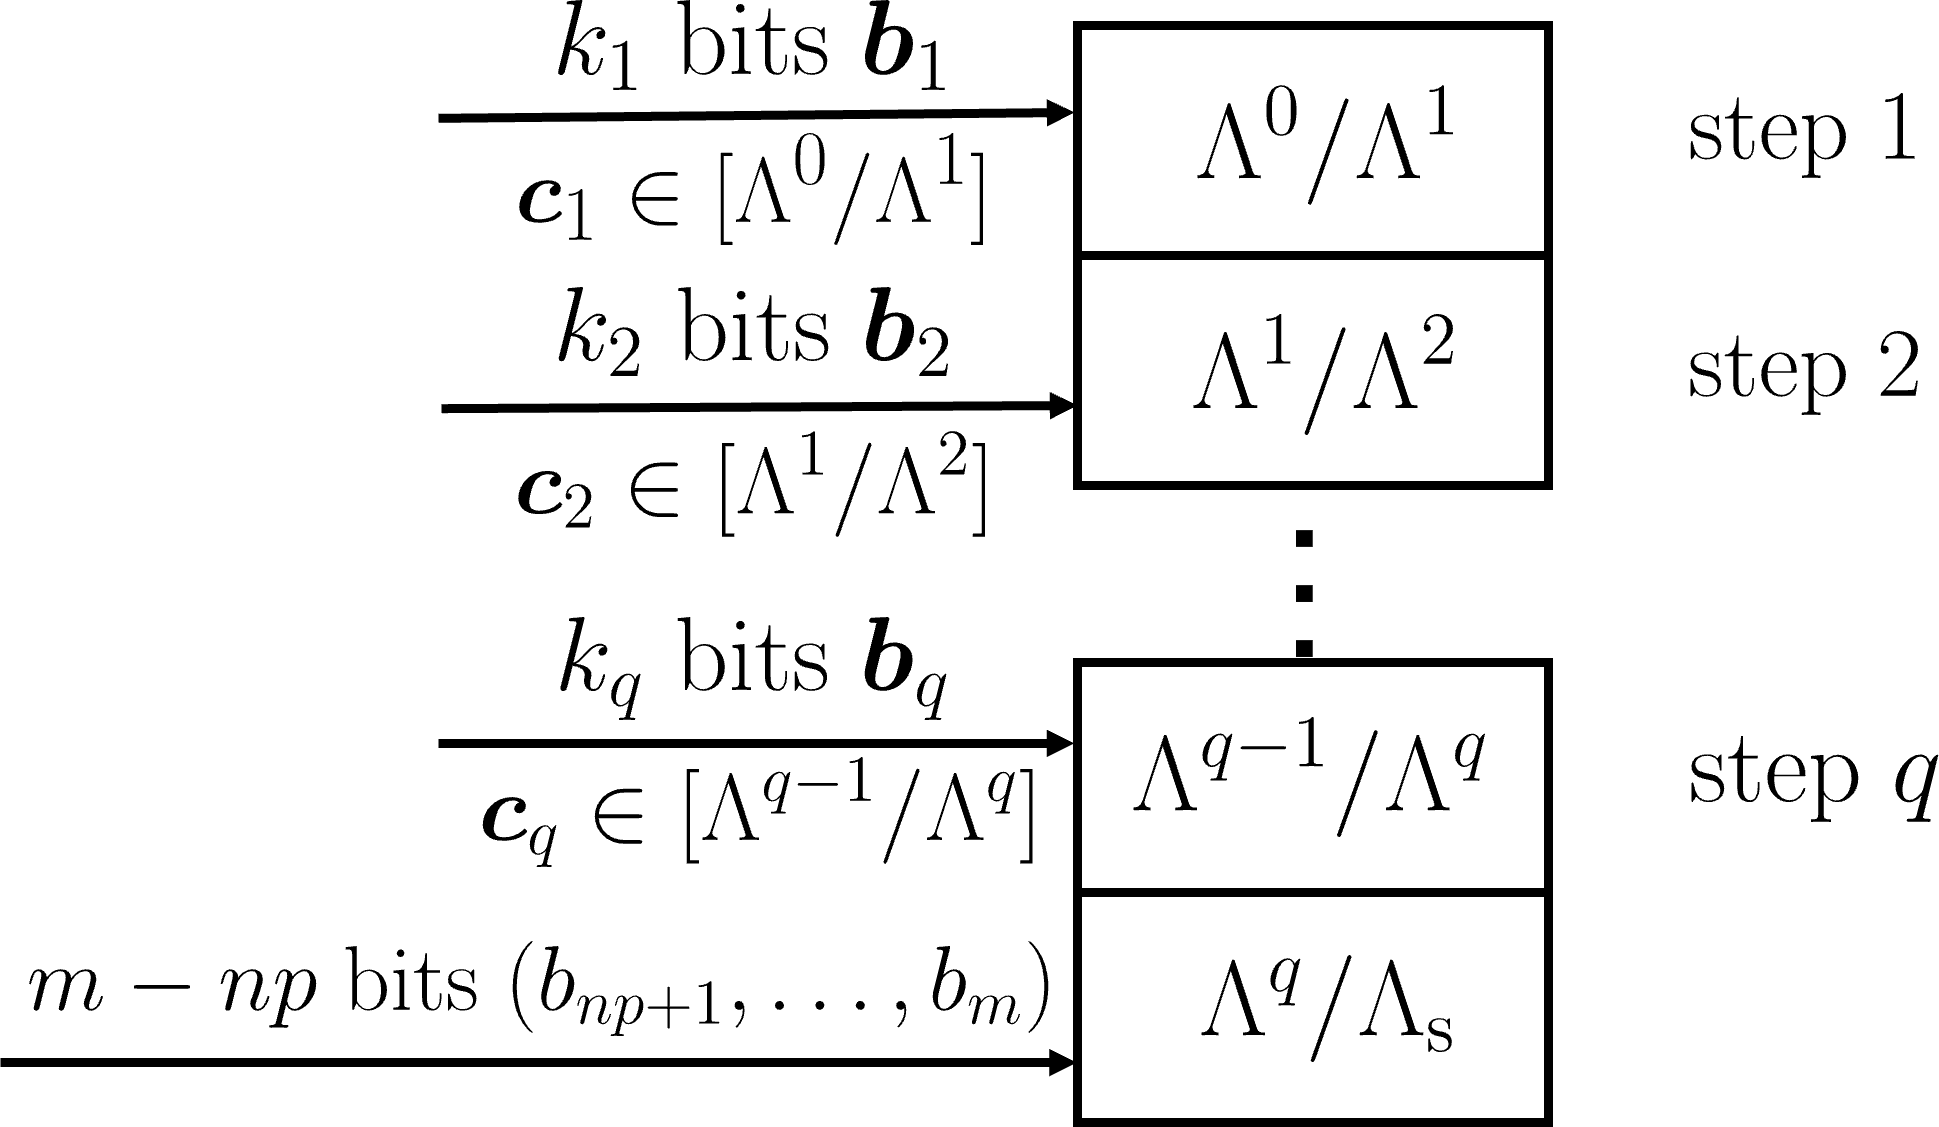
\includegraphics[width=2.6in]{figures/partition_chain.png}
    \caption{Illustration of the labeling of a partition chain $\Lambda^0/\Lambda^1/\dots/\Lambda^{q-1}/\Lambda^q/\Lambdas$.}
    \label{fig:partition chain}
\end{figure}


\begin{table}[tbp]
  % increase table row spacing, adjust to taste
  \renewcommand{\arraystretch}{1.2}
  \renewcommand{\tabcolsep}{12pt}
  \caption{Example partition chains in the SP mapping for MD VCs with a cubic coding lattice $\Z^n$.}
  \label{tab:partition chain}
  \centering
  \begin{tabular}{l l l l l l}
    \hline 
    $n=2$ & \multicolumn{5}{c}{$\Z^2/D_2/2\Z^2/2D_2/4\Z^2/4D_2/\dots$} \\
    \hline 
    Step $i$ & 1 & 2 &3 &4 &5\\
    $k_i$ & 1 & 1& 1 &1&1\\
    $d_i^2$ & 2 &4& 8&16&32\\
    \hline \hline
    $n=4$ & \multicolumn{5}{c}{$\Z^4/D_4/2\Z^4/2D_4/4\Z^4/4D_4/\dots$} \\
    \hline 
    Step $i$ & 1 & 2 &3 &4 &5\\
    $k_i$ & 1 & 1& 1 &1&1\\
    $d_i^2$ & 2 &4& 8&16&32\\
    \hline \hline
    $n=8$ & \multicolumn{5}{c}{$\Z^8/D_8/E_8\bR_{8}/2E_8/2E_8\bR_{8}/4E_8/\dots$} \\
    \hline 
    Step $i$ & 1 & 2 &3 &4 &5\\
    $k_i$ & 1 & 3& 4 &4&4\\
    $d_i^2$ & 2 & 4& 8 &16& 32\\
    \hline \hline
        $n=16$ & \multicolumn{5}{c}{$\Z^{16}/D_{16}/D_{16}\bR_{16}/\Lambda_{16}/\Lambda_{16}\bR_{16}/2\Lambda_{16}/\dots$} \\
    \hline 
    Step $i$ & 1 & 2 &3 &4 &5\\
    $k_i$ & 1 & 8 & 3 & 8 &8\\
    $d_i^2$ & 2 & 4& 8 &16& 32\\
    \hline
  \end{tabular}
\end{table}


\begin{table}[tbp]
  % increase table row spacing, adjust to taste
  \renewcommand{\arraystretch}{1.2}
  \renewcommand{\tabcolsep}{12pt}
  \caption{An example look-up table for the coset representatives of the lattice partition $D_8/E_8\bR_8$ and their bit labels.}
  \label{tab:CosetRep}
  \centering
  \begin{tabular}{l l}
    \hline
    $[D_8/E_8\bR_8]$ & labels \\
    \hline \hline
    $(0 0 0 0 0 0 0 0)$ & $(0 0 0)$\\
    $(0 1 0 1 0 0 0 0)$ & $(0 0 1)$ \\
    $(0 0 0 1 1 0 0 0)$ & $(0 1 0)$ \\
    $(0 1 0 0 1 0 0 0)$ & $(0 1 1)$ \\
    $(1 1 0 0 0 0 0 0)$ & $(1 0 0)$ \\
    $(1 0 0 1 0 0 0 0)$ & $(1 0 1)$ \\
    $(1 1 0 1 1 0 0 0)$ & $(1 1 0)$ \\
    $(1 0 0 0 1 0 0 0)$ & $(1 1 1)$ \\
    \hline
  \end{tabular}
\end{table}
Ungerboeck's SP concept \cite{ungerboeck82} maps binary labels to 1D or 2D constellation points by successively partitioning the constellation into two subsets at each bit level in order to maximize the intra-set minimum squared Euclidean distance (MSED) at each level, so that unequal error protection can be implemented on different bit levels. Since all partition orders are 2, Ungerboeck's SP is also called binary SP. Binary SP has been applied to 1D, 2D \cite{wachsmann99,isaka98,yuan6g21}, and 4D \cite{beygi14jlt,frey20,stern20,stern21} signal constellations. When binary SP is applied in larger than 2 dimensions, the MSED might not increase at every bit level. Binary SP requires one encoder and one decoder at each bit level, which has a high complexity in FEC for large constellations. Generalized from the binary SP, signal sets can be partitioned into multiple subsets based on the concept of cosets \cite{calderbank87,forney88,forney89b,wei87}, which enables SP in higher dimensions \cite{wei87,forney88,forney89b} and increasing MSED at every partition level. How the coset representatives are labeled at each partition level is not specified. In this section, we introduce a systematic algorithm for mapping bits $\bb\in\{0,1\}^m$ to integers $\bu\in\U$ based on SP such that the MSED doubles at every partition level for very large MD VCs based on the lattice partition $\Z^n/\Lambdas$.

For large constellations, after getting a sufficiently large intra-set MSED, it is reasonable to not partition the remaining subsets and leave the corresponding bit levels uncoded. One convenient way is to stop partitioning when a scaled integer lattice $2^p\Z^n$ is obtained, where $p\in \mathbb{N}$. Then we map the last $m-np$ bits to integers according to BRGC to minimize the BER for the uncoded bits.

The preprocessing of the proposed SP mapping works as follows. First, $q$ intermediate lattices $\Lambda^1, \dots, \Lambda^{q}$ are found to form the partition chain
\begin{align} \Lambda^0/\Lambda^1/\dots/\Lambda^{q}/\Lambdas,
\end{align}
where $\Lambda^0=\Z^n$ and $\Lambda^q=2^p\Z^n$ is where to stop the partition. The partition chain should satisfy $\Lambda^0 \supset \Lambda^1 \supset \dots \supset \Lambda^q \supseteq \Lambdas$ and have increasing MSEDs of $d_i^2=2^i$ for ${i=1,\ldots,q}$. The order of each partition step $|\Lambda^{i-1}/\Lambda^i|=2^{k_i}$ for $i=1,\ldots,q$ and $\sum_{i=1}^q k_i= \log_2(|\Lambda^0/\Lambda^q|)=np$. At every partition step $i$, all coset representatives $[\Lambda^{i-1}/\Lambda^i]$ are labeled by $k_i$ bits and the mapping rules are stored in a look-up table $\bC_i$. Conventionally, the set of coset representatives contains the all-zero lattice point labeled by the all-zero binary tuple. Fig.~\ref{fig:partition chain} illustrates the mapping for the partition chain in general. Table~\ref{tab:partition chain} lists some example partition chains and their intra-set MSEDs for MD VCs with a cubic coding lattice. These partition chains contain commonly used lattices as intermediate lattices including the $n$-dimensional checkerboard lattice $D_n$, $8$-dimensional (8D) Gosset lattice $E_{8}$, $16$-dimensional (16D) Barnes--Wall lattice $\Lambda_{16}$ \cite{pook23}, and the $24$-dimensional (24D) Leech lattice $\Lambda_{24}$ \cite[Ch.~4]{conway99book}. The $n\times n$ matrix $\bR_n$ is an integer orthonormal rotation matrix with a determinant of $\det\bR_n=2^{n/2}$ \cite{forney89b, forney88}. When multiplied with a lattice generator matrix on the right, it rotates every two dimensions of the lattice by $\ang{45}$ and rescales it by $\sqrt{2}$. The size of the look-up table $\bC_i$ is $2^{k_i}$, which is not more than $2^8$ in Table~\ref{tab:partition chain} and much smaller than a table for the whole VC.

As an example, a set of coset representatives of the partition $D_8/E_8\bR_8$ and one set of possible bit labels are listed in Table~\ref{tab:CosetRep}. Note that neither the choice of the set of coset representatives nor the mapping within the look-up table is unique, and both of them are arbitrarily selected. The effects of different choices on the performance are not studied. However, we conjecture that there would be no big difference since the intra-set MSED cannot be increased by further partitioning the set of coset representatives.
% For 8- and 16-dimensional lattices, the partition steps are not always two-way, in order to increase the intra-set Euclidean distances at each step. This is different from Ungerboeck's SP for a small constellation. Then the coset representatives are labeled by more than $1$ bit, and can be protected by the same code. 

The SP demapping $f^{-1}_{\text{SP}}$ from an integer vector $\bu$ to its bit labels $\bb$ works as follows. Given an integer vector $\bu \in \U$, starting from the first partition step $\Lambda^0/\Lambda^1$, we know that $\bu$ belongs to one coset of this partition since $\bu\in \Lambda^0=\Z^n$. By full search among a certain set of coset representatives $[\Lambda^0/\Lambda^1]$,  there must be only one $\bc_1\in[\Lambda^0/\Lambda^1]$ such that $(\bu-\bc_1)\cdot\bG_{\Lambda^1}^{-1}$ yields an integer vector, where $\bG_{\Lambda^1}$ is the generator matrix of $\Lambda^1$. The bit labels $\bb_1$ corresponding to $\bc_1$ is found in the look-up table $\bC_1$. Then $\bu-\bc_1$ is a lattice point of $\Lambda^1$, which must belong to a certain coset of $\Lambda^1/\Lambda^2$. A vector $\bc_2\in[\Lambda^1/\Lambda^2]$ is found such that $(\bu-\bc_1-\bc_2)\cdot \bG_{\Lambda^{2}}^{-1}$ yields an integer vector, where $\bG_{\Lambda^{2}}$ is the generator matrix of $\Lambda^2$ and the bit labels $\bb_2$ corresponding to $\bc_2$ is found in the look-up table $\bC_2$. The procedure is repeated until all $\bc_i$ and $\bb_i$ are obtained for $i=1,\ldots,q$. 

Next, the remaining $m-np$ bit labels for the partition $2^p\Z^n/\Lambdas$ are found as follows. First, the coset representatives of the partition $\Z^n/2^p\Z^n$ are set as 
\begin{align}
    \mathcal{S}=[\Z^n/2^p\Z^n]=\{\bs\in\Z^n:\bzero \leq \bs \leq (2^p-1) \cdot \bone\}.\label{eq:SP_coset}
\end{align} 
There must be a unique $\bs\in\mathcal{S}$ such that $\bu-\bs\in 2^p\Z^n$, and $\bs$ can be easily found by 
\begin{align}
    \bs=\bu \bmod 2^p,
\end{align}
where $\bmod$ is the modulo operator that takes the remainder of a vector element-wise and returns a vector. The purpose of choosing such a set of coset representatives is to make sure that $\bu-\bs$ still falls within the range of $\U$, i.e., $\bu-\bs \in \U \cap 2^p\Z^n$. Then we know that
\begin{align}
    \frac{\bu-\bs}{2^p} \in \Z^n
\end{align}
with the range
\begin{align}
    \bzero\leq\frac{\bu-\bs}{2^p}\leq \frac{\bh}{2^p}-\bone.
\end{align}
The bit labels of $(\bu-\bs)/2^p$ can be obtained by converting each decimal element to bits according to BRGC, i.e.,
\begin{align}\label{eq:leftbitsBRGC}
(b_{np+1},\dots,b_m)=f^{-1}_{\text{BRGC}}\left(\frac{\bu-\bs}{2^p},\frac{\bh}{2^p}\right).
\end{align}

Now we describe the SP mapping $f_{\text{SP}}$ from the bit labels $\bb$ to the integer vector $\bu$. Given bit labels $\bb\in\{0,1\}^m$, the first $np$ bits are divided into $q$ blocks $\bb_i$ for $i=1,\ldots,q$, each of which has $k_i$ bits and indicates a coset representative $\bc_i$ according to the look-up $\bC_i$. Then $\bc=\sum_{i=1}^q \bc_i$ indicates a coset representative of the lattice partition $\Z^n/2^p\Z^n$, but $\bc$ might not belong to $\mathcal{S}$, which can be converted to $\bs\in \mathcal{S}$ by
\begin{align}
    \bs=\bc \bmod 2^p.
\end{align}
Now we know that $\bu-\bs\in2^p\Z^n$. The remaining $m-np$ bits of $\bb$ indicate an integer vector
\begin{align}\label{eq:t}
 \bt= f_{\text{BRGC}}\left((b_{np+1},\dots,b_m),\frac{\bh}{2^p}\right).
\end{align}
Finally, $\bu$ is obtained by
\begin{align}\label{eq:u}
    \bu=\bs+2^p\bt.
\end{align}

Algorithms~\ref{Alg:map1} and~\ref{Alg:demap1} summarize the SP mapping process between $\bu$ and $\bb$ for VCs with a cubic coding lattice. 
% After mapping $\bu$ to $\bx$, the intra-set MEDs of the constellation at each partition level should be checked to make sure that they remain the same as of the integer set.

\begin{algorithm}[tbp]
	\caption{SP mapping $f_\text{SP}$}\label{Alg:map1} 
	Input: $\bb$. Output: $\bu$.\\
	Preprocessing: The partition chain $\Lambda^0/\Lambda^1/\dots/\Lambda^q/\Lambdas$ is given, where all partition orders $|\Lambda^{i-1}/\Lambda^i|$ for $i=1,\ldots,q$ are powers of 2. Set the look-up tables $\bC_i$ between all coset representatives and their corresponding bit labels for all partition steps. Divide the first $np$ bits of $\bb$ into $q$ blocks $\bb_i$ for $i=1,\ldots,q$, each of which has $k_i$ bits. Find a lower-triangular generator matrix $\bGs$ of $\Lambdas$ and denote the diagonal elements of $\bGs$ as $\bh$.
	\begin{algorithmic}[1]
        \State Find the corresponding $\bc_i$ of $\bb_i$ according to $\bC_i$ for ${i=1,\ldots,q}$.
	    \State Let $\bc \leftarrow\sum_{i=1}^{q}\bc_i$
            \State Let $\bs \leftarrow \bc- \lfloor\bc/2^p\rfloor \cdot 2^p$
	    \State Let $\bt\leftarrow f_{\text{BRGC}}((b_{np+1},\dots,b_m),\bh/2^p)$
	    \State Let $\bu \leftarrow \bs+2^p\bt$
	\end{algorithmic} 
\end{algorithm}

\begin{algorithm}[tbp]
	\caption{SP demapping $f^{-1}_{\text{SP}}$} \label{Alg:demap1} 
	Input: $\bu$. Output: $\bb$.\\
        The partition chain $\Lambda^0/\Lambda^1/\dots/\Lambda^q/\Lambdas$ is given, where all partition orders $|\Lambda^{i-1}/\Lambda^i|$ are powers of 2. Set the look-up tables $\bC_i$ between all coset representatives and their corresponding bit labels for all steps $i=1,\ldots,q$. Set the set of coset representatives of the partition $\Lambda^0/\Lambda^q$ as $\mathcal{S}$ defined in \eqref{eq:SP_coset}. Find a lower-triangular generator matrix $\bGs$ of $\Lambdas$ and denote the diagonal elements of $\bGs$ as $\bh$.

	\begin{algorithmic}[1]
         \State Let $\bv\leftarrow \bu$
	    \For {$i=1,\ldots,q$}
        \State Find the only $\bc_i \in [\Lambda^{i-1}/\Lambda^i]$ such that $\bu-\bc_i\in\Lambda^i$
        \State Let $\bb_i$ be the bit labels of $\bc_i$ according to $\bC_i$
	\State Let $\bu \leftarrow \bu - \bc_i $
	    \EndFor
        %\State Find the only $\bs \in \mathcal{S}$ such that $\bv-\bs\in\Lambda^q$
        \State Let $\bs\leftarrow \bv \bmod 2^p$
        \State Let $(b_{np+1},\dots,b_m)=f^{-1}_{\text{BRGC}}\left((\bv-\bs)/2^p,\bh/2^p\right)$
        \State Let $\bb\leftarrow(\bb_1,\dots,\bb_{q},b_{np+1},\dots,b_m)$

	\end{algorithmic} 
\end{algorithm}




\subsection{Hybrid mapping}\label{sec:hybrid}

% \begin{figure}[tbp]
%     \centering
%     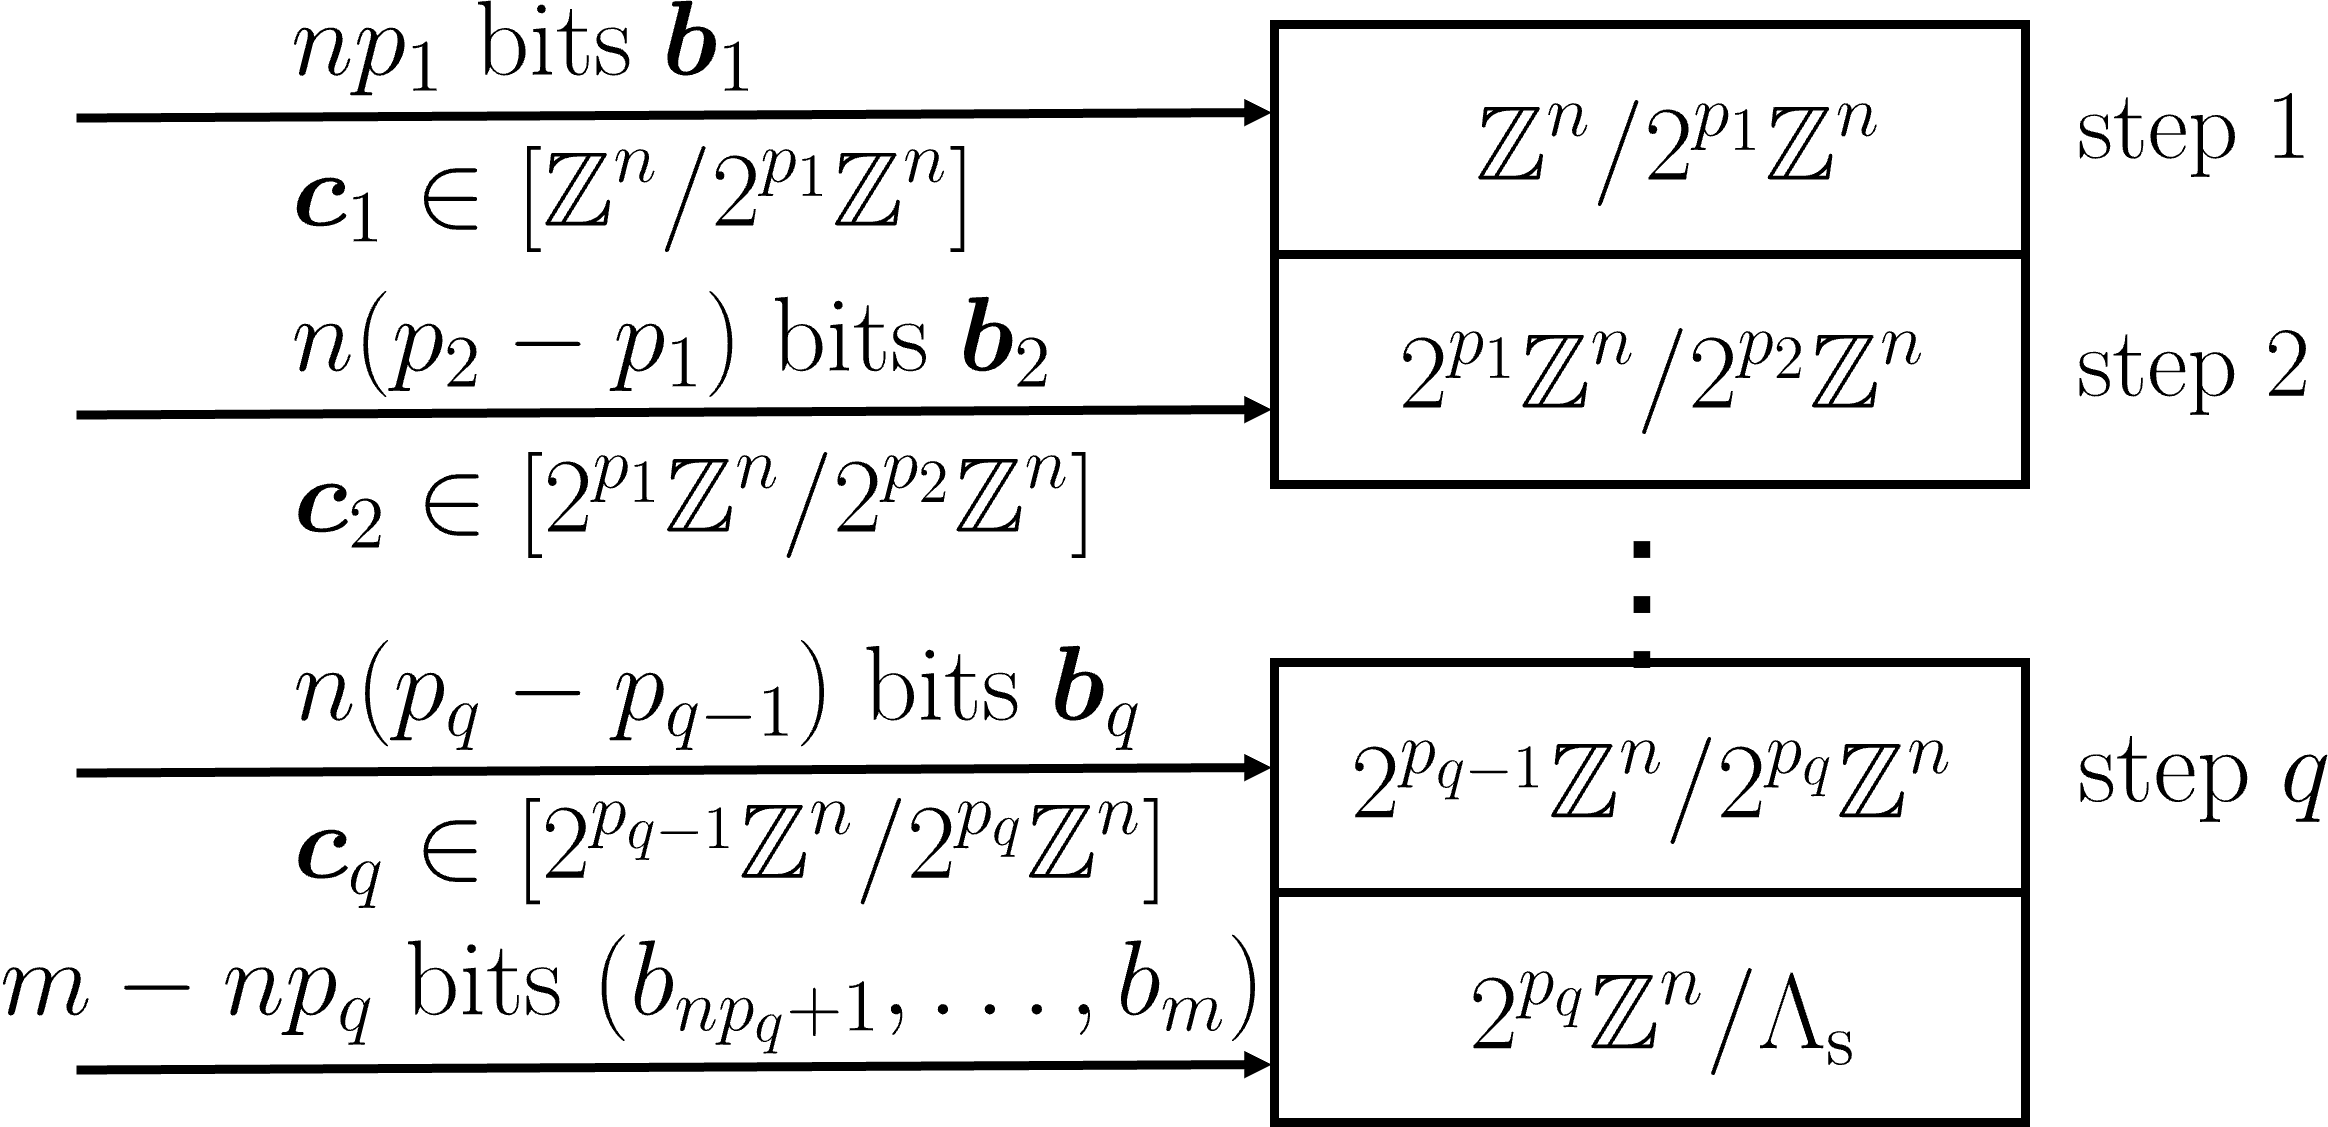
\includegraphics[width=3in]{IEEEtran/hybrid_partition.png}
%     \caption{Illustration of the labeling of the partition chain $\Z^n/2^{p_1}\Z^n/\dots/2^{p_q}\Z^n/\Lambdas$.}
%     \label{fig:hybrid partition}
% \end{figure}
This mapping is a special case of the SP mapping, which is carefully designed for the considered VCs based on the lattice partition $\Z^n/\Lambdas$. The idea is to only consider $q$ intermediate lattices which are a multiple of the cubic lattice, i.e., $\Lambda^i=2^{p_i}\Z^n$ for $i=0,\ldots,q$ with positive integers ${p_1<p_2<\ldots<p_q=p}$ and $p_0=0$. This yields a partition chain $2^{p_0}\Z^n/2^{p_1}\Z^n/2^{p_2}\Z^n/\dots/2^{p_q}\Z^n/\Lambdas$. Thus, the order of each partition step is $|\Lambda^{i-1}/\Lambda^i|=2^{k_i}=2^{n(p_i-p_{i-1})}$ for $i=1,\ldots,q$ and $\sum_{i=1}^q k_i= \log_2(|\Lambda^0/\Lambda^q|)=np$. The intra-set MSED is $d_i^2=2^{p_i}$ at the $i$th partition step. The coset representatives in each partition step is simply set as  
\begin{align}
    \bC_i=[2^{p_{i-1}}\Z^n/2^{p_i}\Z^n]=\{\bc: \bzero \leq \bc \leq (2^{p_{i}-p_{i-1}}-1)\cdot\bone\},\label{eq:coset_reps}
\end{align}
for $i=1,\ldots,q$, which is labeled by $k_i=n(p_i-p_{i-1})$ bits for $i=1,\ldots,q$. Thanks to that these intermediate lattices are a multiple of $\Z^n$, no full search from $\bC_i$ is needed to find the unique coset representative $\bc_i \in \bC_i$ as in the SP mapping. The coset representative $\bc_i$ can be mapped to $n(p_i-p_{i-1})$ bits by directly converting each element of $\bc_i$ to $p_i-p_{i-1}$ bits according to BRGC, i.e.,
\begin{align}
    \bb_i=f^{-1}_{\text{BRGC}}(\bc_i,2^{p_i-p_{i-1}}\cdot\bone),\label{eq:c2b}
\end{align}
for $i=1,\ldots,q$. 
% Fig.~\ref{fig:hybrid partition} shows the hybrid mapping of the partition chain.

The hybrid demapping $f^{-1}_{\text{H}}$ from an integer vector $\bu$ to its bit labels $\bb$ works as follows. Given an integer vector $\bu \in \U$, starting from the first partition step $\Z^n/2^{p_1}\Z^n$, the unique $\bc_1\in\bC_1$ can be easily found by 
\begin{align}
    \bc_1=\bu \bmod 2^{p_1}.
\end{align}
 Then $\bu-\bc_1$ is a lattice point of $2^{p_1}\Z^n$, which must belong to a certain coset of $2^{p_1}\Z^n/2^{p_2}\Z^n$. Then the unique $\bc_2$ is obtained by
 \begin{align}
     \bc_2=(\bu-\bc_1) \bmod 2^{p_2}.
 \end{align}
 Repeating this procedure, $\bc_i$ is found successively by
 \begin{align}\label{eq:ciH}
     \bc_i=\biggl(\bu-\sum_{j=1}^{i-1}\bc_j\biggr) \bmod 2^{p_i}
 \end{align}
 for $i=1,\ldots, q$. Then the first $np$ bit labels of $\bu$ can be obtained by \eqref{eq:c2b}. Similar to the SP mapping, the remaining $m-np$ bits are obtained by \eqref{eq:leftbitsBRGC}, where $\bs=\sum_{i=1}^p \bc_i$ in this case.

% We have ${\bu-\bs \in 2^{p}\Z^n}$. Thus, $(\bu-\bc)/2^{p} \in \Z^n$ with the range
% \begin{align}
%     \bzero\leq\frac{\bu-\bc}{2^{p}}\leq \frac{\bh}{2^{p}}-\bone.
% \end{align}
% The remaining $m-p$ bit labels of $\bu$ can be obtained from converting each decimal element of $(\bu-\bc)/2^{p}$ to bits according to BRGC, i.e.,
% \begin{align}
% (b_{np_q+1},\dots,b_m)=f^{-1}_{\text{BRGC}}\left(\frac{\bu-\bc}{2^{p}},\frac{\bh}{2^{p}}\right).
% \end{align}

The hybrid mapping $f_{\text{H}}$ finding the corresponding integer vector $\bu$ of bit labels $\bb$ works as follows. Given bit labels $\bb\in\{0,1\}^m$, $\bc_i \in \bC_i$ can be directly obtained by
\begin{align}
    \bc_i =f_{\text{BRGC}}(\bb_i,2^{p_i-p_{i-1}}\cdot\bone).\label{eq:b2c}
\end{align}
The integer vector $\bs=\sum_{i=1}^p \bc_i$ must belong to the set $\mathcal{S}$ defined in \eqref{eq:SP_coset} due to the definition of $\bC_i$ in \eqref{eq:coset_reps}. Then $\bu$ is obtained combining \eqref{eq:u} and \eqref{eq:t}. 
% There must be only one integer vector $\bu\in\U$ and one lattice point $\blambda_q\in2^{p}\Z^n$ such that
% \begin{align}
%     \bu=\sum_{i=1}^q\bc_i+\blambda_q.\label{eq:u}
% \end{align}
% We know that the remaining $m-np$ bits indicate an integer vector $\bs$
% \begin{align}
%     \bt=f_{\text{BRGC}}((b_{np+1},\dots,b_m),\bh/2^{p}),\label{eq:s}
% \end{align}
% and 
% \begin{align}
%     \blambda_q=2^{p}\bt.\label{eq:lambdaq}
% \end{align}


Algorithms~\ref{Alg:map2} and~\ref{Alg:demap2} summarize the hybrid mapping process between $\bu$ and $\bb$ for VCs with a cubic coding lattice. 
% For effective partition of the constellation, after mapping $\bu$ to $\bx$, the intra-set MED of the constellation at the $i$th partition step should be checked to make sure to be $2^{p_i}$ for $i=1,\ldots,q$. 
\begin{algorithm}[tbp]
	\caption{Hybrid mapping $f_{\text{H}}$}\label{Alg:map2} 
	Input: $\bb$. Output: $\bu$.\\
       Preprocessing: Given the partition chain $2^{p_0}\Z^n/2^{p_1}\Z^n/2^{p_2}\Z^n/\dots/2^{p_q}\Z^n/\Lambdas$ with positive integers ${p_1<p_2<\ldots<p_q=p}$ and $p_0=0$, set $q$ sets of coset representatives $\bC_i$ as in \eqref{eq:coset_reps} for $i=1,\ldots,q$. Divide the first $np$ bits of $\bb$ into $q$ blocks $\bb_i$ for $i=1,\ldots,q$, each of which has $n(p_i-p_{i-1})$ bits. Find a lower-triangular generator matrix $\bGs$ and denote the diagonal elements of $\bGs$ as $\bh$.
	\begin{algorithmic}[1]
	    \State Let $\bc_i \leftarrow f_{\text{BRGC}}(\bb_i,2^{p_i-p_{i-1}}\cdot\bone)$ for $i=1,\ldots,q$
     \State Let $\bs \leftarrow \sum_{i=1}^q\bc_i$
	    \State Let $\bt \leftarrow f_{\text{BRGC}}\left((b_{np+1},\ldots,b_{m}),\bh/2^{p}\right)$
	    \State Let $\bu \leftarrow \bs +2^{p}\bt$
	\end{algorithmic} 
\end{algorithm}

\begin{algorithm}[tbp]
	\caption{Hybrid demapping $f^{-1}_{\text{H}}$} \label{Alg:demap2} 
	Input: $\bu$. Output: $\bb$.\\
       Preprocessing: Given the partition chain $2^{p_0}\Z^n/2^{p_1}\Z^n/2^{p_2}\Z^n/\dots/2^{p_q}\Z^n/\Lambdas$ with positive integers ${p_1<p_2<\ldots<p_q=p}$ and $p_0=0$, set $q$ sets of coset representatives $\bC_i$ as in \eqref{eq:coset_reps} for $i=1,\ldots,q$. Find a lower-triangular generator matrix $\bGs$ and denote the diagonal elements of $\bGs$ as $\bh$.
	\begin{algorithmic}[1]
           \For {$i=1,\ldots,q$}
        % \State Find the only $\bc_i \in [2^{p_{i-1}}\Z^n/2^{p_{i}}\Z^n]$ such that ${\bu-\bc_i\in2^{p_i}\Z^n}$
        \State Let $\bc_i=\bu \bmod 2^{p_i}$
        \State Let $\bb_i \leftarrow f^{-1}_{\text{BRGC}}(\bc_i,2^{p_i-p_{i-1}}\cdot\bone)$
	\State Let $\bu \leftarrow \bu - \bc_i $
	    \EndFor
        \State Let $\left(b_{np+1},\ldots,b_{m}\right) \leftarrow f^{-1}_{\text{BRGC}}(\bu/2^{p},\bh/2^{p})$
        \State Let $\bb=(\bb_1,\ldots,\bb_q,b_{np+1},\dots,b_m)$
	\end{algorithmic} 
\end{algorithm}



\emph{Example 1:} A simple example is a 2D VC based on the lattice partition $\Z^n/4D_2$, where $4D_2$ is the scaled 2D checkerboard lattice with the generator matrix
\begin{align}
\bGs=\begin{pmatrix}
8 & 0\\ 
4 & 4
\end{pmatrix}.\notag
\end{align}
This VC does not provide any shaping gain, which is just for simplicity of illustration. Fig.~\ref{Fig:labeling} illustrates the three different mapping rules $f$ for this example VC. It can be observed that all integer points have only 1-bit difference from their nearest neighbors in the Gray mapping. The SP mapping is based on the lattice partition chain $\Z^2/D_2/2\Z^2/4D_2$ ( $q=2$, $p=1$). The hybrid mapping is based on the lattice partition chain $\Z^2/2\Z^2/4D_2$ ($q=p=1$), and ${[\Z^n/2\Z^n]=\{(0,0),(1,0),(0,1),(1,1)}\}$. For both SP and hybrid mapping, within each coset of $2\Z^2/4D_2$, the points have only 1-bit difference among the last three bits from their closest neighbors. 

\begin{figure}[tbp]
\centering
\begin{subfigure}{\linewidth}
    \centering
    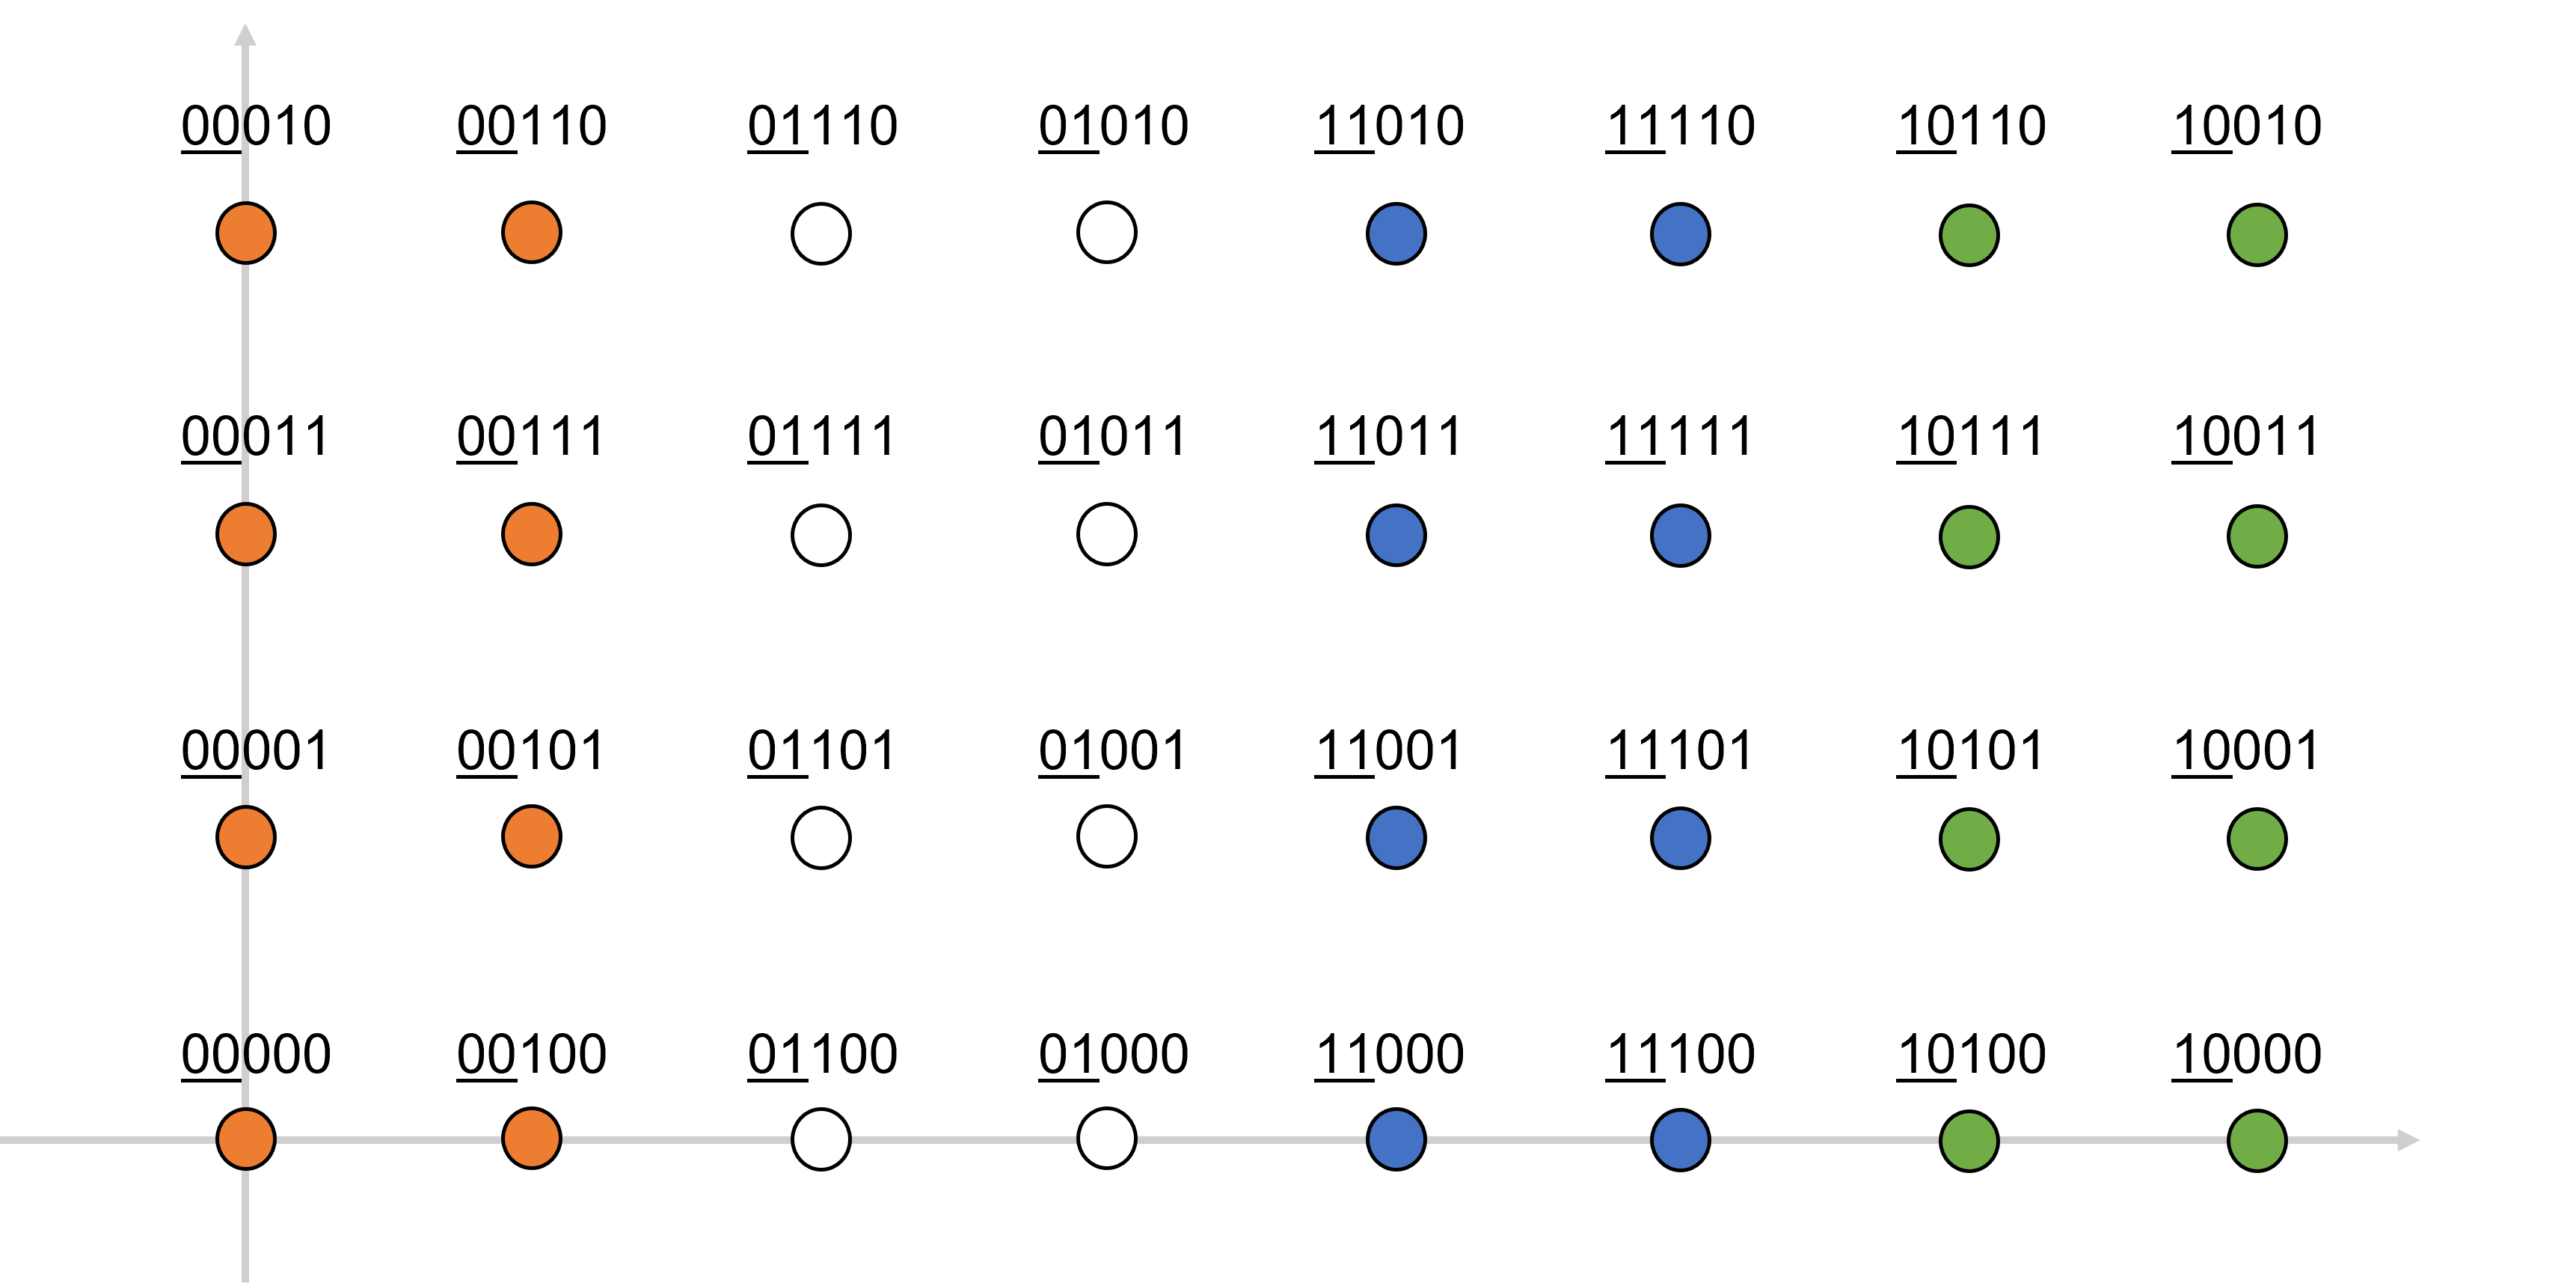
\includegraphics[width=3.5in]{figures/labeling1.png}
    \caption{Gray mapping}
    \label{Fig:labeling1}
    \end{subfigure}
    \begin{subfigure}{\linewidth}
        \centering
        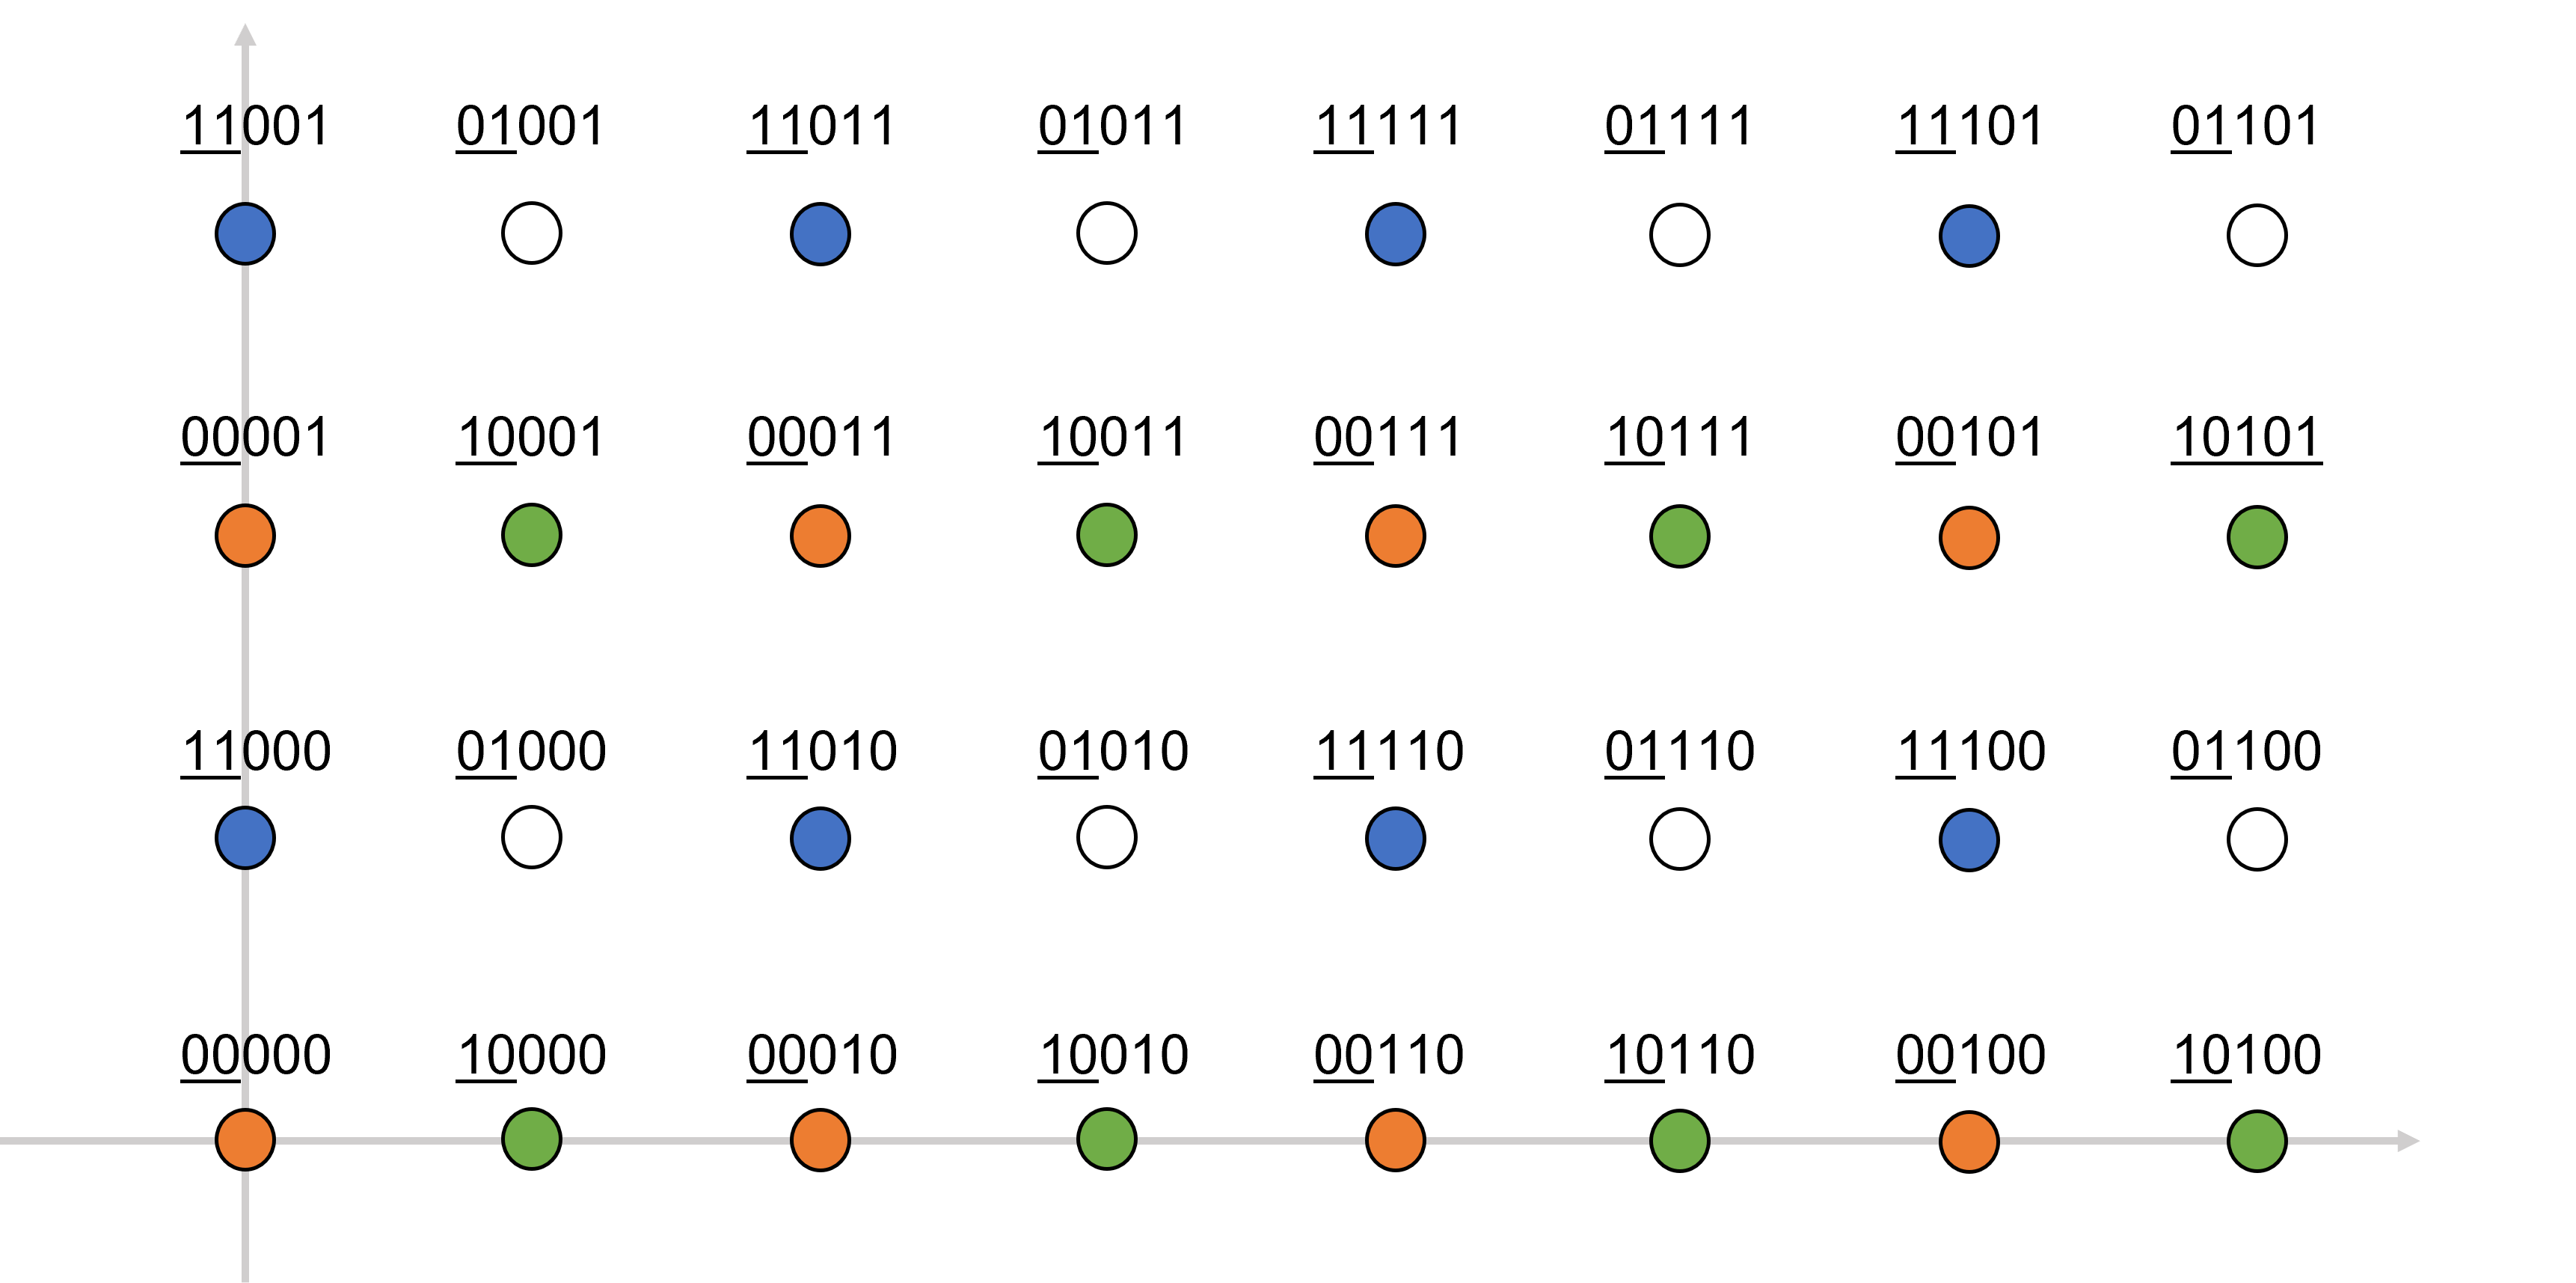
\includegraphics[width=3.5in]{figures/labeling2.png}%
        \caption{SP mapping}
        \label{Fig:labeling2}
    \end{subfigure}
    \begin{subfigure}{\linewidth}
        \centering
        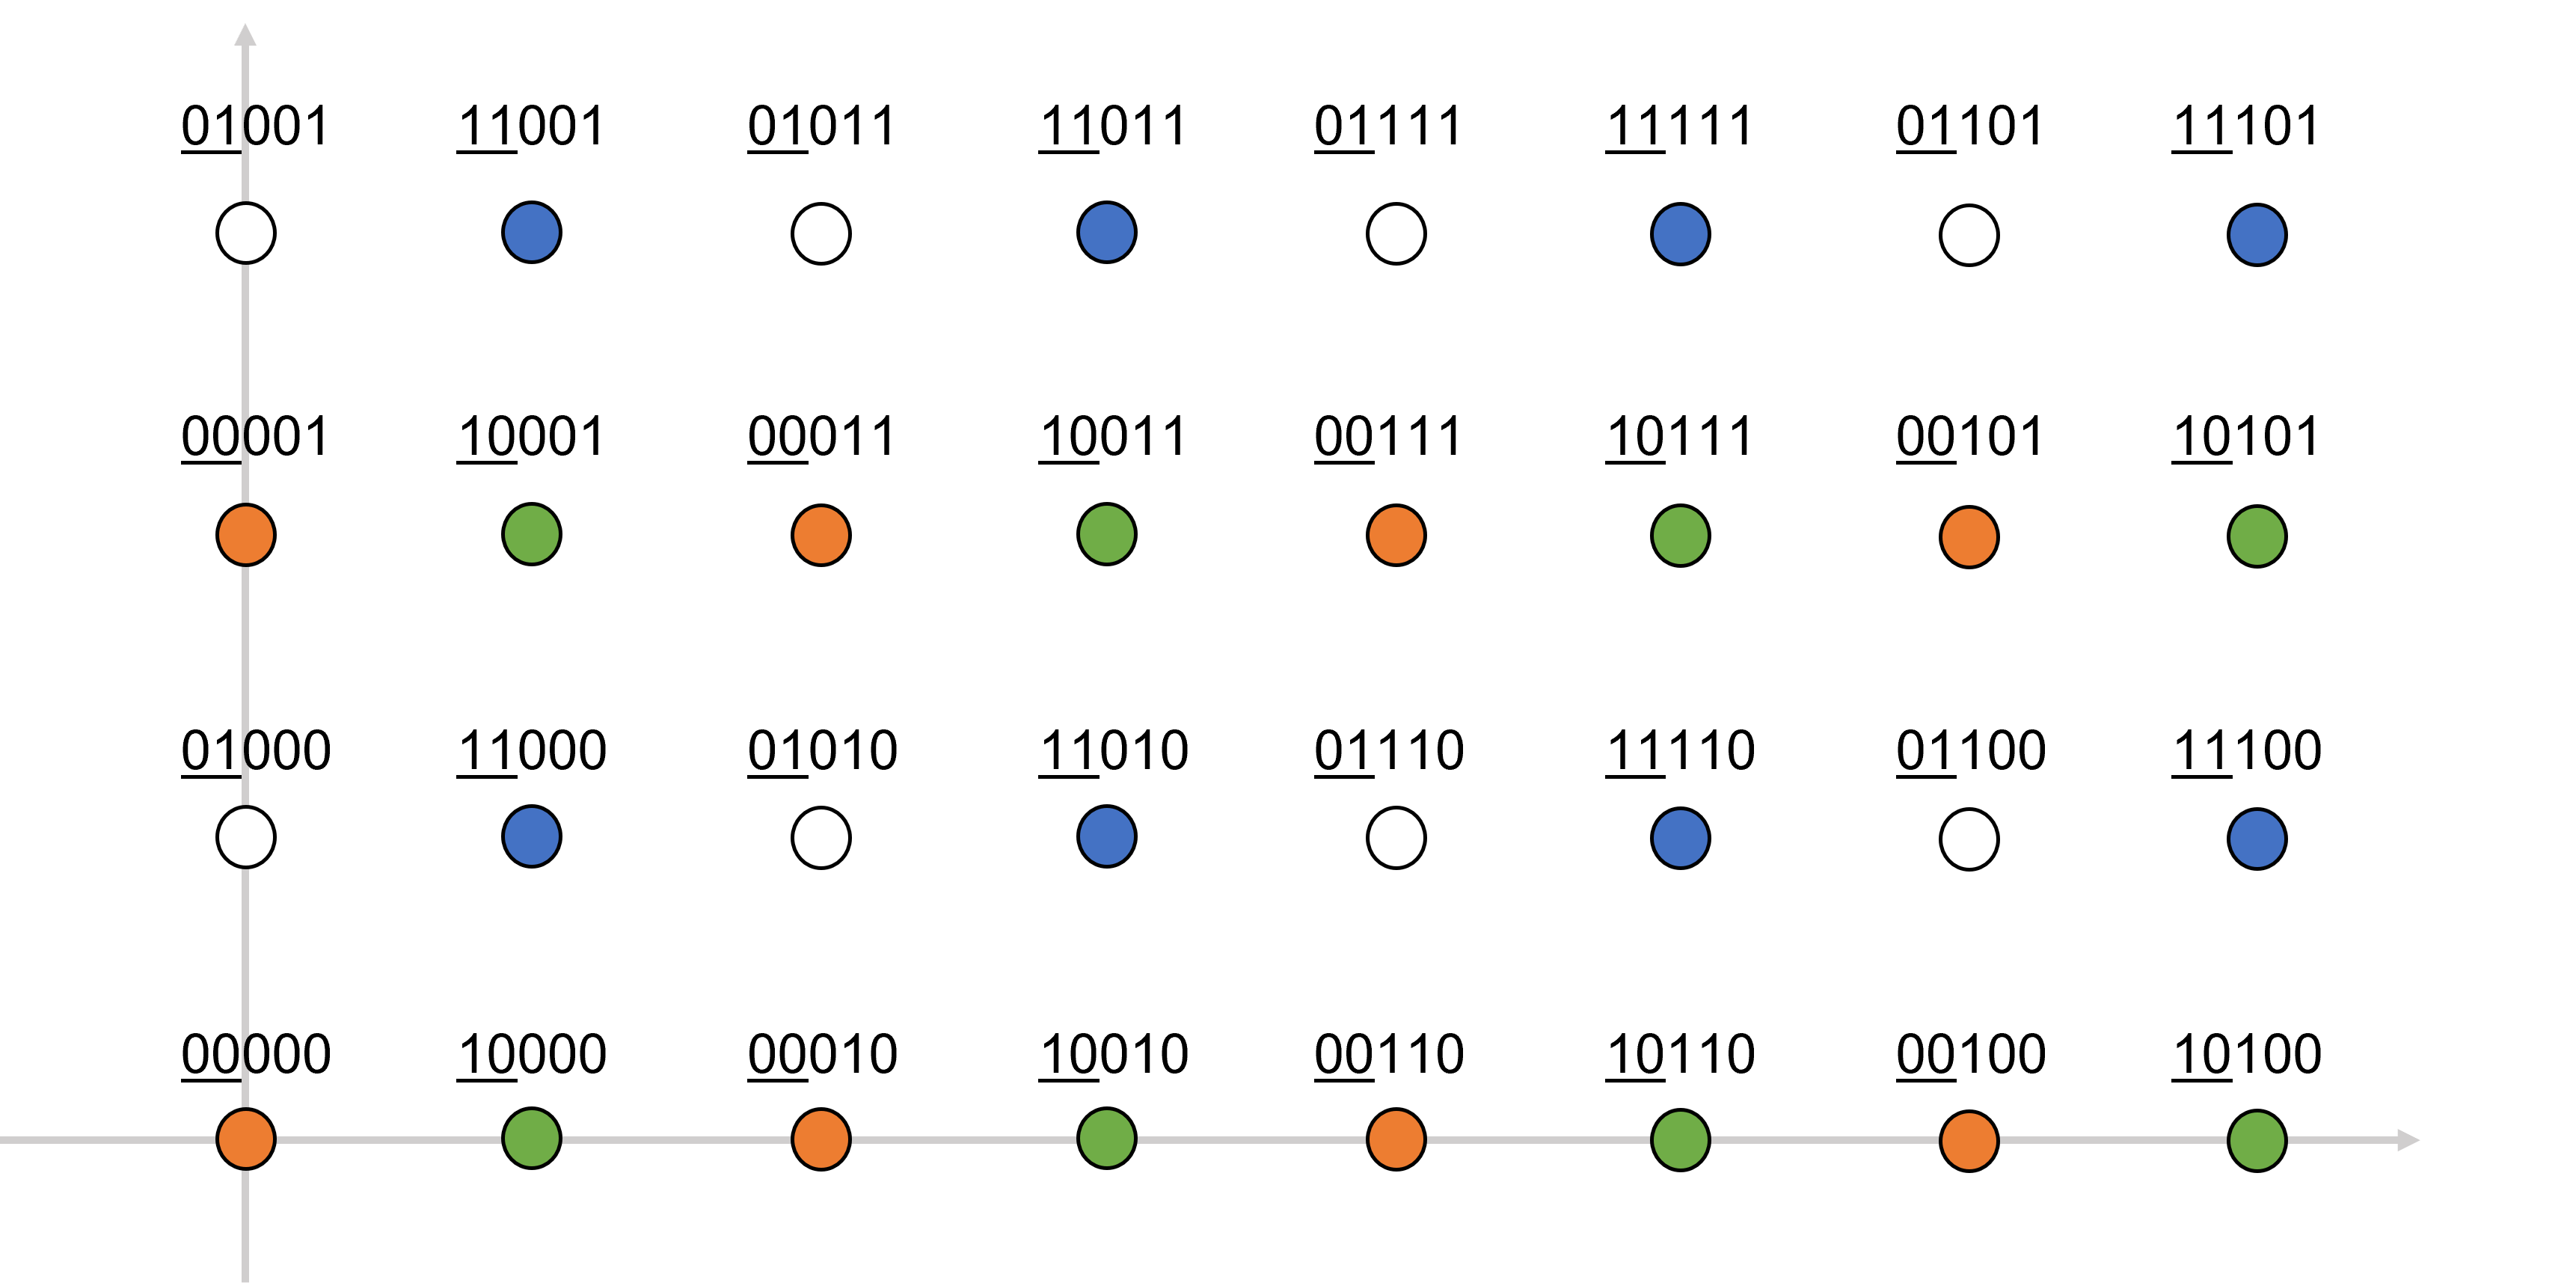
\includegraphics[width=3.5in]{figures/labeling3.png}%
        \caption{Hybrid mapping}
        \label{Fig:labeling3}
    \end{subfigure}
    \caption{Example 1: Different mapping rules $f$ between integer vectors and bit labels for the VC based on the lattice partition $\Z^2/4D_2$. Integer points having the same first two bits are filled with the same color for better visualization and comparison.}
    \label{Fig:labeling}
\end{figure}



\section{CM schemes}\label{sec:CM}
% The study in \cite{ourjlt} already shows that VCs can achieve power gains over QAM at both for the AWGN channel and the power gains of VCs over QAM have already shown. This makes a coding scheme with a single HDcode combining with the pre-FEC prediction suitable for VCs achieving power gains after decoding. 

The joint design of forward error correction (FEC) coding and modulation formats is called coded modulation (CM), which plays a vital part in modern communication systems. Designing a CM scheme involves a trade-off among the spectral efficiency, power, and complexity. In this section, we propose three SD CM schemes for VCs based on the lattice partition $\Z^n/\Lambdas$, adopting the three labeling schemes introduced in section~\ref{sec:labeling}, and the computation of the log-likelihood ratios (LLRs) for SD decoding is discussed.

The designed CM schemes can be combined with an outer hard-decision (HD) code, known as concatenated coding \cite{forney1965concatenated,barakatain2020}. Concatenated codes are widely used in many communication standards nowadays, such as the DVB-S2 standards \cite{dvbs2} for satellite communications and the 400ZR \cite{400ZR} and upcoming 800G standards for fiber-optical communications \cite{stern21}. The inner CM scheme brings the uncoded BER down to a certain target BER (e.g., around $10^{-3}$ for fiber-optic communications). Then the outer code can further eliminate the error floor and achieve a very low BER as needed. Commonly used outer codes include Reed--Solomon codes \cite{wicker1999reed}, turbo product codes \cite{wang23}, Bose--Chaudhuri--Hocquenghem codes \cite{forney1965bch}, staircase codes \cite{smith2011staircase}, and zipper codes \cite{sukmadji2019zipper}.
% For the design of CM schemes for VCs, we adopt this concatenated coding structure and focuses on the inner CM scheme design.
% Concatenated codes \cite{forney1965concatenated} balances this trade-off well and is commonly used in many communication standards nowadays, such as the DVB-S2 standards \cite{dvbs2} for satellite communications, the 400ZR \cite{400ZR} and upcoming 800G standards for fiber-optical communications. It combines a hard-decision (HD) outer code and a soft-decision (SD) inner code, with an interleaver in between sometimes. The inner code brings the uncoded BER down to a certain target BER of the outer code (e.g. around $10^{-3}$ for fiber-optic communications). Then, the outer code can further eliminate the error floor and achieve a very low BER as needed. Commonly used outer codes include Reed-Solomon codes, Bose–Chaudhuri–Hocquenghem codes, and staricase codes. The inner codes can be convolutional codes, low-density parity check (LDPC) codes, and Hamming codes.
\begin{figure*}[tbp]
\centering
\begin{subfigure}{\linewidth}
    \centering
    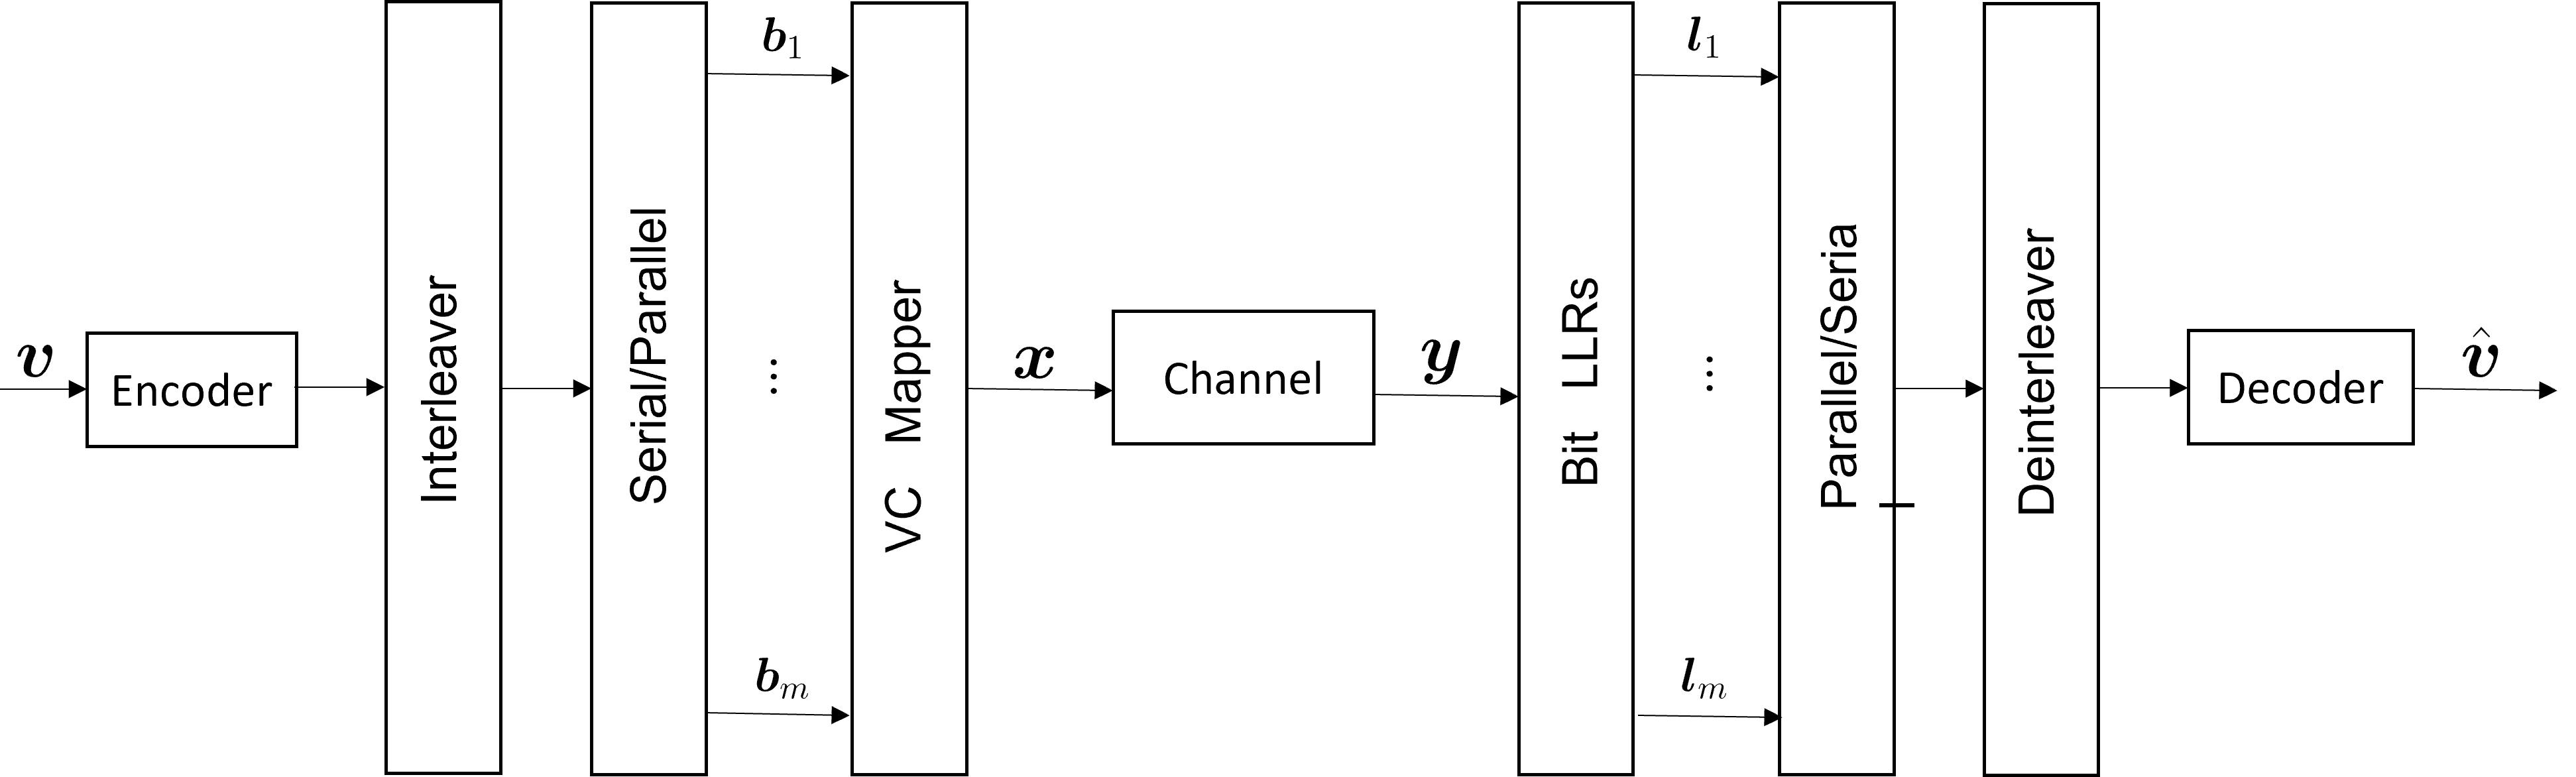
\includegraphics[width=5.4in]{figures/BICM.png}
    \caption{BICM: A block of $N\Rc$ information bits $\bv$ are encoded into $N$ bits by the encoder and then permuted by the interleaver to avoid burst errors \cite{caire98}. The serial bits after interleaving are converted to $m$ parallel bit streams $\bb_1,\ldots,\bb_m$ of length $N/m$. At the time slot $j=1,\ldots,N/m$, a VC mapper first maps $m$ bits $\bb^j=(b_1^j,\dots,b_m^j)$ to an integer $\bu^j$ by $\bu^j=f_{\text{BRGC}}\left(\bb^j,\bh\right)$, and then maps $\bu^j$ to a VC point $\bx^j \in \Gamma$ by $\bx^j=g(\bu^j)$. The receiver deinterleaves $N$ independent LLRs of the bits and then uses them to decode $\hat{\bv}$.}
    \label{Fig:BICM}
    \end{subfigure}
    \begin{subfigure}{\linewidth}
        \centering
        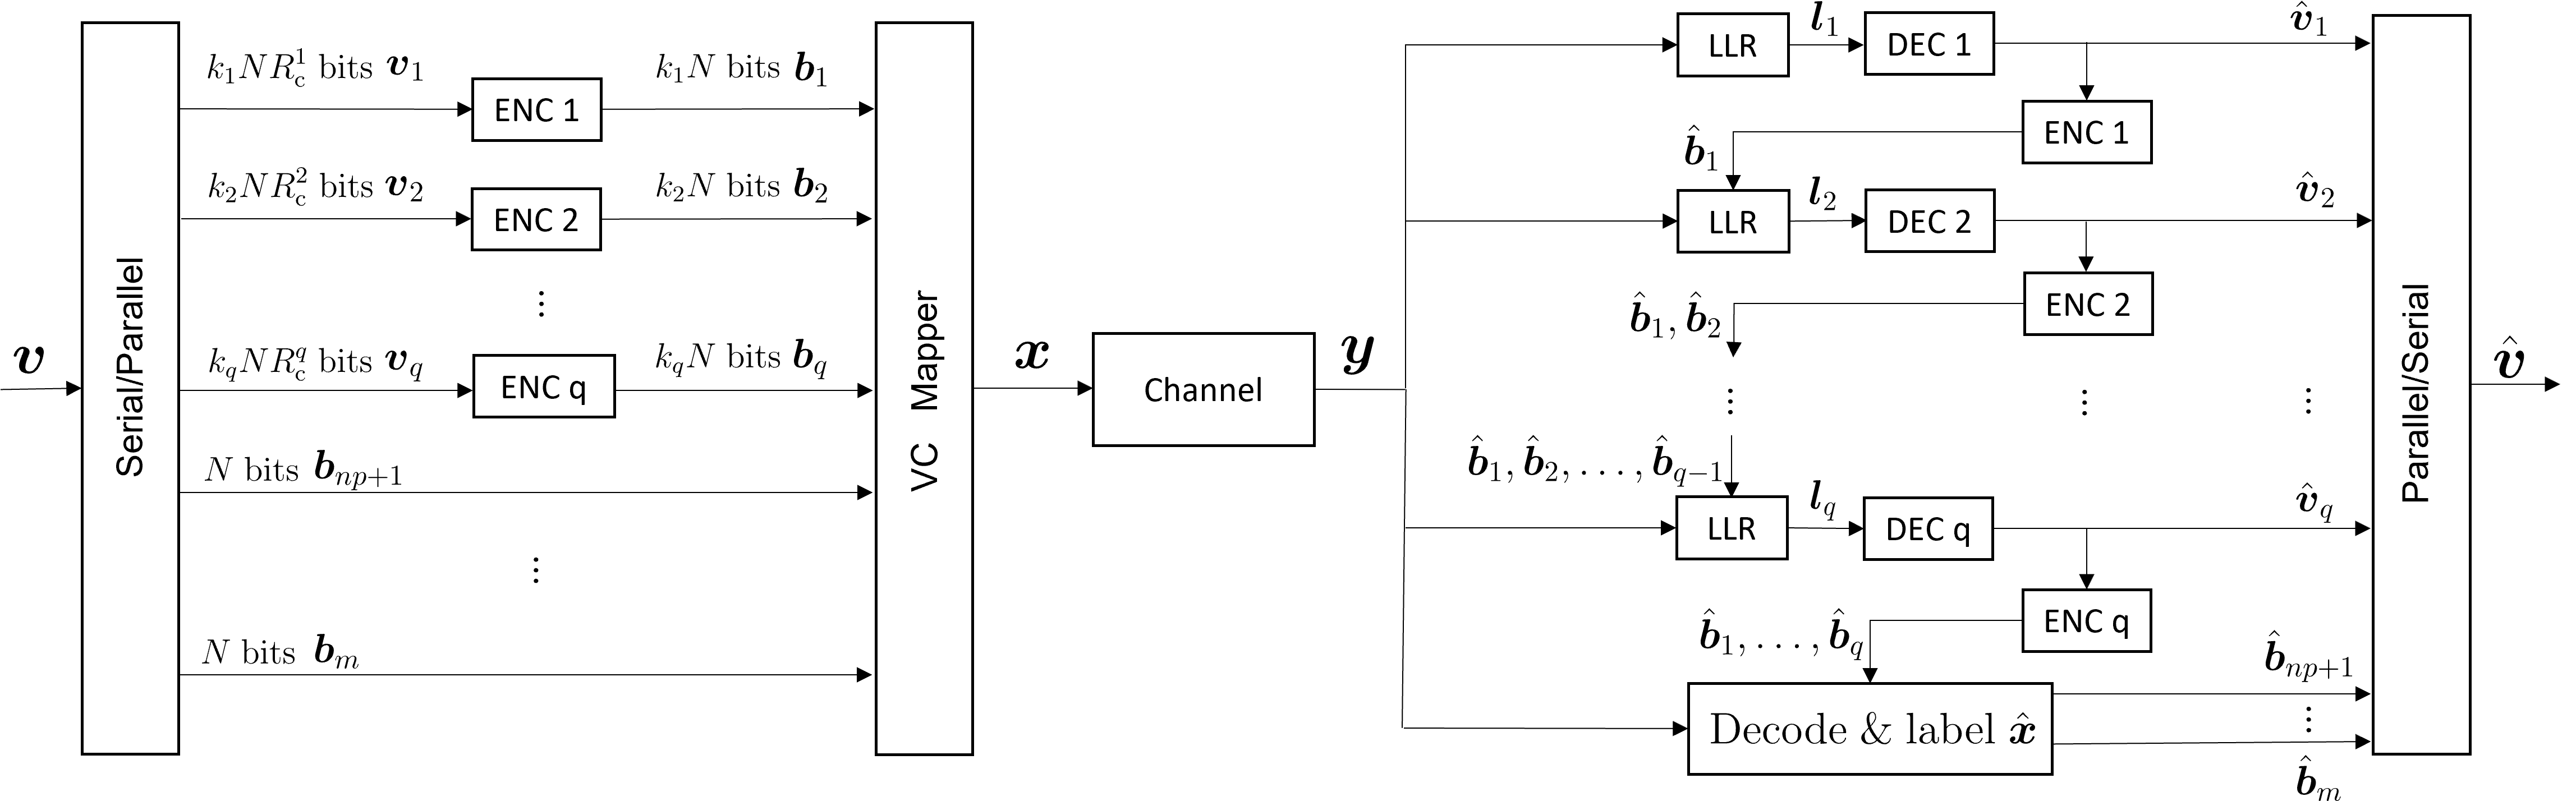
\includegraphics[width=7in]{figures/MLCM.png}%
        \caption{MLCM: A block of serial information bits $\bv$ are partitioned into $q$ parallel bit streams $\bv_i$ with $k_iN\Rc^{i}$ bits for $i=1,\ldots,q$ and $m-np$ parallel uncoded bit streams $\bb_{np+1},\ldots,\bb_m$ with length $N$. Then $\bv_i$ is encoded into $k_iN$ bits $\bb_i$ by encoder (ENC) $i$ for $i=1,\ldots,q$. The VC mapper first maps bits to $N$ integer vectors by the SP or hybrid mapping, and then encode these integer vectors into $N$ VC points $\bx$. Multistage decoding is performed at the receiver after receiving $N$ noisy symbols $\by$. Decoder (DEC) 1 first decodes $k_1N\Rc^1$ bits $\hat{\bv}_1$ back based on $\by$ and $k_1N$ LLRs $\bl_1$. Then $\hat{\bv}_1$ is encoded into $\hat{\bb}_1$ by encoder 1. Decoder $i=2,\ldots,q$ successively decodes $\hat{\bv}_i$ and reencodes it into $\hat{\bb}_i$ based on $\by$ and LLRs $\bl_i$, given all previous bits $\hat{\bb}_1,\dots,\hat{\bb}_{i-1}$. The estimation of the uncoded bits $\hat{\bb}_{np+1},\ldots,\hat{\bb}_m$ is obtained after getting $\hat{\bb}_1,\dots,\hat{\bb}_{q}$.}
        \label{Fig:MLCM}
    \end{subfigure}
    \caption{Block diagrams of BICM and MLCM for VCs.}
    \label{Fig:CM}
\end{figure*}

% The gap between \eqref{eq:MI} and \eqref{eq:GMI} is determined by the labeling, and becomes rather small for independent Gray labeling.
% The MI in \eqref{eq: MI} implies a multilevel coded modulation (MLCM) scheme, where unequal protection is implemented to different bit levels a The MI and GMI are the fundamental limits of the two typical CM schemes, multilevel coded modulation (MLCM) and bit-interleaved coded modulation (BICM), respectively. 

\subsection{BICM for VCs with Gray mapping}
Consider a channel with input symbols $\bX$ labeled by $m$ bits $(\bB_1,\dots,\bB_m)$ and output symbols $\bY$. The mutual information (MI) between $\bX$ and $\bY$ is
\begin{align}\label{eq:MI}
    I(\bY;\bX)&=I(\bY;\bB_1,\dots,\bB_m) \notag\\ &=I(\bY;\bB_1)+I(\bY;\bB_2|\bB_1)+\dots \notag\\
    &+I(\bY;\bB_m|\bB_1,\dots,\bB_{m-1}) 
\end{align}
according to the chain rule. If the conditions in all conditional MIs of \eqref{eq:MI} are neglected, the BICM capacity \cite{agrell11}
\begin{align}
     I_{\text{BMI}}&=\sum_{i=1}^{m}I(\bY;\bB_i)\leq I(\bY;\bX)\label{eq:GMI}
\end{align}
is obtained. The channel is regarded as $m$ independent bit subchannels, which can be encoded and decoded independently. BICM utilizes this concept and contains only one binary component code to protect all bit subchannels. An interleaver is added between the encoder and symbol mapper to distribute the coded bits evenly to all bit subchannels.

The Gray mapping in Section~\ref{sec:pseudo} maps each bit level independently, and is suitable to be combined with BICM. Fig.~\ref{Fig:BICM} illustrates the BICM scheme for VCs. 
% The information bits $\bv$ are encoded by the inner encoder and then permuted by the interleaver to avoid burst errors \cite{caire98}. The serial (S) bits after interleaving are converted to $m$ parallel (P) bit streams $\bb_1,\ldots,\bb_m$. At the $j$th time slot, a VC mapper first maps $m$ bits $\bb^j=(b_1^j,\dots,b_m^j)$ to an integer $\bu^j$ by $\bu^j=f_{\text{BRGC}}\left(\bb^j,\bh\right)$, and then maps $\bu^j$ to a VC point $\bx^j \in \Gamma$ by $\bx^j=g(\bu^j)$. The receiver deinterleaves the independent LLRs of the bits and then uses them to decode $\hat{\bv}$. 
The total rate of BICM for VCs is $\beta \Rc$ [bits/2D-symbol], where $\Rc$ is the code rate of the inner code. Decoding is based on bit LLRs, which is described below.

For a constellation $\Gamma$ transmitted over the AWGN channel, the max-$\log$ approximation \cite{viterbi98} of the $k$th bit after receiving a $\by^j\in\R^n$ for $j=1,\ldots,N/m$ is defined as
\begin{align}
    \text{LLR}(b_{k}|\by^j)=  -\frac{1}{\sigma^2}\left (\min_{\bx\in\Gamma^{(k,0)}}\|\by^j-\bx\|^2- \min_{\bx\in\Gamma^{(k,1)}}\|\by^j-\bx\|^2\right),\label{eq:IndependentLLR}
\end{align}
where $\sigma^2$ is the noise power per two dimensions, $\Gamma^{(k,0)}$ and $\Gamma^{(k,1)}$ are the sets of constellation points 
with 0 and 1 at bit position $k$, respectively, and $\Gamma^{(k,0)}\cup \Gamma^{(k,1)}=\Gamma$. Computing \eqref{eq:IndependentLLR} needs a full search in $\Gamma$, which is infeasible for very large constellations. In \cite{ourTC}, an LLR approximation method based on importance sampling is proposed and exemplified for very large VCs based on the lattice partition $\Z^n/\Lambdas$ for the AWGN channel. The idea is to only search from a small portion of the whole constellation, which is called ``importance set''. In this paper, instead of searching from a subset of the VC, we further reduce the complexity of the approximation in \cite[Eq. (33)]{ourTC} by searching from a finite number of lattice points from $\Z^n-\ba$ that are inside a ``Euclidean ball'' centered at $\lfloor\by^j+\ba\rceil$, i.e.,
\begin{align}\label{eq:ball}
    \B(\by^j,R^2)\triangleq\{\be:\|\be+\ba-\left \lfloor \by^j+\ba  \right \rceil\|^2 \leq R^2, \be+\ba \in \Z^n\},
\end{align}
where $\lfloor\cdot\rceil$ represents rounding a vector to its nearest integer vector and $R^2\ge 0$ is the squared radius of the Euclidean ball. When the SNR is low, the points in the Euclidean ball might partially or fully fall outside of the constellation boundary. Compared with the method in \cite[Eq. (33)]{ourTC}, where the importance set is defined as $\B(\by^j,R^2)\cap \Gamma$, searching among all points from $\B(\by^j,R^2)$ might return a point outside $\Gamma$, which causes a loss in decoding performance. However, the computation complexity is reduced a lot since no closest lattice point quantizer needs to be applied to all points in $\B(\by^j,R^2)$ in order to determine the intersection with $\Gamma$.

The bit labels of the points in the Euclidean ball ${\be\in\B(\by^j,R^2)}$ can be obtained by 
\begin{align}
    f^{-1}_{\text{BRGC}}\left(w(\be),\bh)\right).
\end{align}
Then for each bit position $k$, $\B(\by^j,R^2)$ can be divided into two subsets $\B(\by^j,R^2)=\B^{(k,0)}(\by^j,R^2)\cup\B^{(k,1)}(\by^j,R^2)$, containing points within $\B(\by^j,R^2)$ with 0 and 1 at bit position $k$, respectively.
Thus, the approximated max-$\log$ LLRs $\bl^j$ of the $j$th channel realization $\by^j$ contain $m$ independent values $l_k^j$ for $k=1,\ldots,m$. The LLR of the $k$th bit is computed as
\begin{align}\label{eq:LLR_EUball}
    l_k^j=&-\frac{1}{\sigma^2}\biggl(\min_{\be\in\B^{(k,0)}(\by^j,R^2)}\|\by+\ba-\be\|^2 \notag \\&- \min_{\be\in\B^{(k,1)}(\by^j,R^2)}\|\by+\ba-\be\|^2\biggr).
\end{align}
% If $\B^{(i,0)}(\by,R^2)=\varnothing$, then set ${\min_{\be\in \B^{(i,0)}(\by,R^2)}\|\by-\be\|^2}$ to a large default value $r>R^2$. The same rule applies to $\B^{(i,1)}(\by,R^2)$. 
If either $\B^{(k,0)}(\by^j,R^2)$ or $\B^{(k,1)}(\by^j,R^2)$ is empty, then the corresponding minimum in \eqref{eq:LLR_EUball} is set to a large default value $r>R^2$. Here only integer values of $R^2$ are considered, because the ${\| \be+\ba-\lfloor \by^j+\ba \rceil \|^2}$ in \eqref{eq:ball} is always an integer. The choice of $R^2$ involves a trade-off between computation complexity and decoding performance. For high-dimensional VCs, the LLR approximation can have high complexity when the Euclidean ball contains a larger number of points. Given $R^2$, $r$ can be roughly optimized by testing which value gives the best decoding performance.

\subsection{MLCM for VCs with SP mapping}
Denoting the terms of \eqref{eq:MI} as $I_1,\ldots,I_m$, a channel can be regarded as $m$ virtual independent ``equivalent subchannels'' with MIs
\begin{align}\label{eq:Ii}
    I_k=I(\bY;\bB_k|\bB_1,\dots,\bB_{k-1})
\end{align}
for $k=1,\ldots,m$. This concept directly implies an MLCM scheme proposed by Imai \emph{et al.} in \cite{imai77}, where the bit subchannels are protected unequally with different component channel codes and a multistage decoder decodes the bits successively from $\bB_1$ to $\bB_m$ provided that the previous bits are given. Practical design rules of the code rates can be found in \cite{wachsmann99}. The suitable labeling for MLCM is Ungerboeck's SP labeling. 

Fig.~\ref{Fig:MLCM} shows an MLCM scheme for VCs, which contains $q$ component codes with code rates $\Rc^i$ for $i=1,\ldots,q$ and the same codeword length $N$ to protect the first $np$ bit levels of the VC symbols, and the last $m-np$ bit levels remain uncoded. Thus, the MLCM for VCs has a total rate of
\begin{align}
    R_{\text{tot}}= \frac{\sum_{i=1}^qk_i\Rc^i+(m-np)}{n/2} \text{[bits/2D-symbol].}
\end{align}
The transmitter forms $m$ bits $\bb^{j}=(\bb_1^j,\ldots,\bb_q^j,b_{np+1}^j,\dots,b_m^j)$ for $j=1,\ldots,N$, where $\bb_i^j=(b_i^{k_i(j-1)+1},\ldots,b_i^{k_ij})$ are the $(k_i(j-1)+1)$th to $k_ij$th bits of $\bb_i$ for $i=1,\ldots,q$. The $\bb_i$ is illustrated in Fig.~\ref{Fig:MLCM} with length $k_iN$ for $i=1,\ldots,q$. For the SP mapping, the VC mapper first maps $\bb^j$ to an integer by $\bu^j=f_{\text{SP}}(\bb^j)$ and then encodes the integer into a VC point by $\bx^j=g(\bu^j)$. 

% After receiving $\by^j \in \R^n$, which is a noisy version of $\bx^j$, decoder 1 first decodes $\hat{\bv}_1^j$, and then $\hat{\bv}_1^j$ is encoded into $\hat{\bb}_1^j$ by encoder 1. Decoder $i$ successively decodes $\hat{\bb}_i^j$ based on $\by^j$, given all previous bits $\hat{\bb}_1^j,\dots,\hat{\bb}_{i-1}^j$, from $i=2$ to $q$. 

At the receiver side, after getting $(\hat{\bb}_1^j,\dots,\hat{\bb}_q^j)$, the coset representative $\hat{\bc}_i^j$ is obtained according to $\bC_i$ for $i=1,\ldots,q$, and the $\hat{\bc}^j\in[\Z^n/2^p\Z^n]$ is found by $\hat{\bc}^j=\sum_{i=1}^q \hat{\bc}_i^j$. Then the estimation of the transmitted point should be found by searching a point within the subset $2^p\Z^n+\hat{\bc}^j$ that is closest to $\by^j+\ba$. This is equivalent to
\begin{align}
    \hat{\bx}^j &=\Q_{2^p\Z^n+\hat{\bc}^j}(\by^j+\ba)\notag\\
    &=2^p\left\lfloor\frac{\by^j+\ba-\hat{\bc}^j}{2^p} \right\rceil+\hat{\bc}^j-\ba.\label{eq:xhat}
\end{align}
Finally, the bit labels of $\hat{\bx}^j$ are obtained by 
\begin{align}\label{eq:bhatSP}
   \hat{\bb}^j=(\hat{\bb}_1^j,\ldots,\hat{\bb}_q^j,\hat{b}_{np+1}^j,\ldots,\hat{b}_m^j)= f_{\text{SP}}^{-1}(w(\hat{\bx}^j)),
\end{align}
where the last $m-np$ bits $(\hat{b}_{np+1}^j,\ldots,\hat{b}_m^j)$ are the estimation of the uncoded bits mapped to $\hat{\bx}^j$.

The max-log LLRs of $\bb_i^j$ contains $k_i$ LLR values independent of each other, denoted by $\bl_i^j=(l_{i,1}^j,\dots,l_{i,k_i}^j)$, which is computed by the following procedure. Given $\hat{\bb}_1^j,\dots,\hat{\bb}_{i-1}^j$, the coset representatives $\hat{\bc}_1^j,\dots,\hat{\bc}_{i-1}^j$ are directly obtained according to look-up tables $\bC_{1},\dots,\bC_{i-1}$. Then we know that the corresponding integer belongs to the lattice $\Lambda^{i-1}+\sum_{t=1}^{i-1}\hat{\bc}_t^j$. In the $i$th partition step, the coset representatives $[\Lambda^{i-1}/\Lambda^i]$ have been labeled by the look-up table $\bC_i$. Then we can divide $\bC_i$ into two subsets $\bC_i=\bC_i^{(e,0)}\cup\bC_i^{(e,1)}$, representing coset representatives having a bit 0 and 1 at the $e$th bit of $\bb_i$, respectively. For all $\hat{\bc}_i^j\in\bC_i^{(e,0)}$, we find the closest point to $\by+\ba$ from the lattice $\Lambda^i+\sum_{t=1}^{i-1}\hat{\bc}_t^j+\hat{\bc}_i^j$, and denote all such closest points as the set
\begin{align}
    \mathcal{Z}_i^{(e,0)}=\{&\bz=\Q_{\Lambda^i+\sum_{t=1}^{i}\hat{\bc}_t^j}(\by+\ba):\hat{\bc}_i^j \in \bC_i^{(e,0)}\}.
\end{align}
The set $\mathcal{Z}_i^{(k,1)}$ is defined analogously. Then the max-log LLR of the $e$th bit of $\bb_i^j$ can be approximated as 
\begin{align}
    &\text{LLR}\left(b_i^j|\by, \hat{\bb}_1^j,\dots,\hat{\bb}_{i-1}^j\right)\approx l_{i,e}^j\notag\\
    &=-\frac{1}{\sigma^2}\left (\min_{\bz\in\mathcal{Z}_i^{(e,0)}}\|\by+\ba-\bz\|^2- \min_{\bz\in\mathcal{Z}_i^{(e,1)}}\|\by+\ba-\bz\|^2\right).\label{eq:LLR_MLC}
\end{align}
The computation complexity of the LLRs in MLCM depends on the partition orders $k_i$, which is much lower than the complexity of \eqref{eq:LLR_EUball} in BICM. However, MLCM uses $q$ component codes, which adds complexity and delay compared with BICM.
\begin{table}[tbp]
  % increase table row spacing, adjust to taste
  \renewcommand{\arraystretch}{1.4}
  \renewcommand{\tabcolsep}{3.2pt}
  \caption{The considered VCs and TDHQ formats in the simulation.}
  \label{tab:VCs}
  \centering
  \begin{tabular}{c c c c c c}
    \hline 
    Name &$n$& $\Lambda/\Lambdas$ &  $M$  & $m$ & $\beta$ \\
    \hline \hline
    $E_8^{24}$ &8& $\Z^8/8E_8$ & $16,777,216$& 24 &6\\
    $\Lambda_{24}^{72}$ &24 &$\Z^{24}/2\Lambda_{24}\bR_{24}$ & $\approx4.7\times10^{21}$& 72 &6\\
    $E_8^{32}$ &8& $\Z^8/16E_8$ & $\approx4.3\times10^{9}$& 32 &8\\
    $\Lambda_{24}^{96}$ &24& $\Z^{24}/4\Lambda_{24}\bR_{24}$ & $\approx7.9\times10^{28}$& 96 &8\\
    $E_8^{40}$ &8& $\Z^8/32E_8$ & $\approx1.1\times10^{12}$& 40 &10\\
    $\Lambda_{24}^{120}$ &24& $\Z^{24}/8\Lambda_{24}\bR_{24}$ & $\approx1.3\times10^{36}$& 120 &10\\
    $E_8^{48}$ &8& $\Z^8/64E_8$ & $\approx2.8\times10^{14}$& 48 &12\\
    $\Lambda_{24}^{144}$ &24& 16$\Z^{24}/4\Lambda_{24}\bR_{24}$ & $\approx2.2\times10^{43}$& 144 &12\\
    $\Lambda_{16}^{76}$ &16& $\Z^{16}/16\Lambda_{16}$ & $\approx7.9\times10^{22}$ & 76 &9.5\\
    $\Lambda_{16}^{92}$ &16& $\Z^{16}/32\Lambda_{16}$ & $\approx5.0\times 10^{27}$ & 92 &11.5\\
    \hline
    Name &  $t_1,t_2$ &$M_1,M_2$  & 
    $m_{\text{QAM}}$ & $\beta_{\text{QAM}}$ \\
    \hline \hline
    TDHQ1 & 4, 4 &512,1024 &76 & 9.5\\
    TDHQ1 & 4, 4 &2048,1096 &92 & 11.5\\
    \hline
  \end{tabular}
\end{table}

\begin{table*}[tbp]
  % increase table row spacing, adjust to taste
  \renewcommand{\arraystretch}{1.3}
  \renewcommand{\tabcolsep}{1.2pt}
  \caption{The parameters of the considered CM schemes in simulation.}
  \label{tab:CMparameters}
  \centering
  \begin{tabular}{c c c c c c c c c}
    \hline 
    Constellation & Mapping & $\beta$ & CM & Partition chain&$\#$LDPC codes & Code rates & $\#$Coded bit levels/$m$ & $R_{\text{tot}}$ [2D-symbol] \\
    \hline \hline 
    $E_8^{24}$ & Gray & 6& BICM& -& 1 &$\Rc=8/9$ &24/24 & 5.33\\
    64-QAM & Gray & 6& BICM &-& 1 &$\Rc=8/9$ &6/6 & 5.33\\
    $E_8^{24}$ & hybrid & 6& MLCM &$\Z^{8}/2\Z^{8}/E_{8}^{24}$& 1 &$\Rc^1=2/3$ &8/16 & 5.33\\
    $\Lambda_{24}^{72}$ & hybrid & 6& MLCM &$\Z^{24}/2\Z^{24}/\Lambda_{24}^{72}$& 1 &$\Rc^1=2/3$ &24/48 & 5.33\\
    64-QAM & hybrid & 6& MLCM &-& 1 &$\Rc^1=2/3$ &2/6 & 5.33\\
    \hline
    $E_8^{32}$ & Gray & 8& BICM& -& 1 &$\Rc=9/10$ &32/32 & 7.2\\
    256-QAM & Gray & 8& BICM &-& 1 &$\Rc=9/10$ &8/8 & 7.2\\
    $E_8^{32}$ & hybrid & 8& MLCM &$\Z^8/2\Z^8/E_8^{32}$& 1 &$\Rc^1=3/5$ &8/24 & 7.2\\
    $\Lambda_{24}^{96}$ & hybrid & 8& MLCM &$\Z^{24}/2\Z^{24}/\Lambda_{24}^{96}$& 1 &$\Rc^1=3/5$ &24/72 & 7.2\\
    256-QAM & hybrid & 8& MLCM &-& 1 &$\Rc^1=3/5$ &2/8 & 7.2\\
    256-QAM & SP & 8& MLCM &-& 2 &$\Rc^1=1/3, \Rc^2=8/9$ &2/8 & 7.22\\
    \hline
    $E_8^{40}$ & Gray & 10& BICM& -& 1 &$\Rc=9/10$ &40/40 & 9\\
    1024-QAM & Gray & 10& BICM &-& 1 &$\Rc=9/10$ &10/10 & 9\\
    $E_8^{40}$ & hybrid & 10& MLCM &$\Z^8/2\Z^8/E_8^{40}$& 1 &$\Rc^1=1/2$ &8/40 & 9\\
    $\Lambda_{24}^{120}$ & hybrid & 10& MLCM &$\Z^{24}/2\Z^{24}/\Lambda_{24}^{120}$& 1 &$\Rc^1=1/2$ &24/120 & 9\\
    1024-QAM & hybrid & 10& MLCM &-& 1 &$\Rc^1=1/2$ &2/10 & 9\\
    \hline
    $E_8^{48}$ & Gray & 12& BICM& -& 1 &$\Rc=9/10$ &48/48 & 10.8\\
    4096-QAM & Gray & 12& BICM &-& 1 &$\Rc=9/10$ &12/12 & 10.8\\
    $E_8^{48}$ & hybrid & 12& MLCM &$\Z^8/2\Z^8/E_8^{48}$& 1 &$\Rc^1=2/5$ &8/48 & 10.8\\
    $\Lambda_{24}^{144}$ & hybrid & 12& MLCM &$\Z^{24}/2\Z^{24}/\Lambda_{24}^{144}$& 1 &$\Rc^1=2/5$ &24/144 & 10.8\\
    4096-QAM & hybrid & 12& MLCM &-& 1 &$\Rc^1=2/5$ &2/12 & 10.8\\
    $E_8^{48}$ & SP & 12& MLCM &$\Z^8/D_8/E_8\bR_8/2\Z^8/E_8^{48}$& 1 &$\Rc^1=0,\Rc^2=0,\Rc^3=4/5$ &8/48 & 10.8\\
    \hline 
    $\Lambda_{16}^{92}$ & Gray & 11.5& BICM & -&1 &$\Rc=9/10$ &92/92 & 10.35\\
    TDHQ2 & Gray & 11.5& BICM & -&1 &$\Rc=9/10$ &92/92 & 10.35\\
    $\Lambda_{16}^{92}$ & hybrid & 11.5& MLCM &$\Z^{16}/2\Z^{16}/\Lambda_{16}^{92}$& 1 &$\Rc^1=2/5$ &16/92 & 10.3\\
    TDHQ2 & hybrid & 11.5& MLCM &-& 1 &$\Rc^1=2/5$ &16/92 & 10.3\\
    
    \hline
  \end{tabular}
\end{table*}

\subsection{MLCM for VCs with hybrid mapping}
The MLCM scheme for VCs with the hybrid mapping in Section~\ref{sec:hybrid} is a special case of Fig.~\ref{Fig:MLCM} with $p=p_q$ and $k_i=n(p_i-p_{i-1})$. At time step $j=1,\ldots,N$, the VC mapper maps $m$ bits $\bb^j=(\bb_1^j,\ldots,\bb_q^j,b_{np+1}^j,\ldots,b_m^j)$ to an integer $\bu^j =f_{\text{H}}(\bb^j)$ and then maps $\bu^j$ to a VC point $\bx^j=g(\bu^j)$. At the receiver side, successive decoding is performed based on $\by^j$ and all previous bits $(\hat{\bb}_1^j,\dots,\hat{\bb}_{i-1}^j)$ for decoder $i$. After decoding $(\hat{\bb}_1^j,\dots,\hat{\bb}_{q}^j)$, the coset representative $\hat{\bc}_i^j$ is obtained by \eqref{eq:b2c} for $i=1,\ldots,q$. The estimation of the coset representative of the partition $\Z^n/2^p\Z^n$ is calculated as $\hat{\bs}^j=\sum_{i=1}^q \hat{\bc}_i^j$. The estimation of the transmitted VC point $\hat{\bx}^j$ is decoded by \eqref{eq:xhat}, where $\hat{\bc}^j$ is replaced by $\hat{\bs}^j$. Finally, the estimation of bit labels of $\hat{\bx}^j$ is obtained by 
\begin{align}\label{eq:bhatH}
   \hat{\bb}^j=(\hat{\bb}_1^j,\ldots,\hat{\bb}_q^j,\hat{b}_{np+1}^j,\ldots,\hat{b}_m^j)= f_{\text{H}}^{-1}(w(\hat{\bx}^j)),
\end{align}
where the last $m-np$ bits $(\hat{b}_{np+1}^j,\ldots,\hat{b}_m^j)$ are the estimation of the uncoded bits mapped to $\bx^j$. The hybrid CM scheme for VCs has a total rate of
\begin{align}
    R_{\text{tot}}= \frac{\sum_{i=1}^q n(p_i-p_{i-1})\Rc^i+(m-np)}{n/2} \text{[bits/2D-symbol].}
\end{align}

The max-log LLRs of $\bb_i^j=(b_{i,1}^j,\dots,b_{i,n(p_i-p_{i-1})}^j)$ contain $n(p_i-p_{i-1})$ independent LLR values for $i=1,\ldots,q$, denoted by $\bl_i^j=(l_{i,1}^j,\dots,l_{i,n(p_i-p_{i-1})}^j)$ and calculated as follows. Given the previous estimated bits $\hat{\bb}_1,\dots,\hat{\bb}_{i-1}$, the coset representatives $\bc_t$ for $t=1,\ldots,i-1$ are obtained by \eqref{eq:b2c}. If $|2^{p_{i-1}}\Z^n/2^{p_i}\Z^n|$ is not a very large number, the max-log LLR of the $e$th bit of $\bb_i^j$, denoted by $l_{i,e}^j$, can be calculated using \eqref{eq:LLR_MLC} with ${\Lambda^{i-1}=2^{p_{i-1}}\Z^n}$ and ${\Lambda^i=2^{p_i}\Z^n}$. If $|2^{p_{i-1}}\Z^n/2^{p_i}\Z^n|$ is large, then $l_{i,e}^j$ can be calculated by enumerating a scaled Euclidean ball centered at the closest lattice point of $2^{p_{i-1}}\Z^n$ to $\by$, i.e.,
\begin{align}
    \D(\by,R^2)\triangleq\biggl\{&\be:\|\be+\ba-\left \lfloor \frac{\by+\ba}{2^{p_{i-1}}}  \right \rceil \cdot 2^{p_{i-1}} \|^2 \leq 2^{2p_{i-1}}R^2, \notag \\ &\be+\ba \in 2^{p_{i-1}}\Z^n\biggr\},\label{eq:D}
\end{align}
which consists of two subsets $\D(\by,R^2)=\D(\by,R^2)^{(e,0)}\cup\D(\by,R^2)^{(e,1)}$, representing points with $0$ and $1$ at the $e$th bit of $\bb_i$, respectively. Then $l_{i,e}^j$ is computed as
\begin{align}\label{eq:LLR_Hybrid}
        l_{i,e}^j=&-\frac{1}{\sigma^2}\biggl(\min_{\be\in\D^{(e,0)}(\by^j,R^2)}\|\by+\ba-\be\|^2 \notag \\&- \min_{\be\in\D^{(e,1)}(\by^j,R^2)}\|\by+\ba-\be\|^2\biggr).
\end{align}

It is worth noting that, when $p_i=i$ for $i=1,\ldots,q$ (i.e., the partition chain $\Z^n/2\Z^n/\dots/2^q\Z^n/\Lambdas$ is considered), setting $R^2=1$ in \eqref{eq:LLR_Hybrid} is sufficient, thanks to \eqref{eq:coset_reps} and \eqref{eq:c2b} in the hybrid labeling. The approximation complexity will be very low since $\D(\by,1)$ contains only $2n+1$ points. Also, $\D^{(e,0)}(\by,1)$ or $\D^{(e,1)}(\by,1)$ can never be an empty set for $i=1,\ldots,n$, due to \eqref{eq:coset_reps} and \eqref{eq:c2b} again.




%
% \subsection{Subsection Heading Here}
% Subsection text here.
%
% needed in second column of first page if using \IEEEpubid
%\IEEEpubidadjcol
%
%
% An example of a floating figure using the graphicx package.
% Note that \label must occur AFTER (or within) \caption.
% For figures, \caption should occur after the \includegraphics.
% Note that IEEEtran v1.7 and later has special internal code that
% is designed to preserve the operation of \label within \caption
% even when the captionsoff option is in effect. However, because
% of issues like this, it may be the safest practice to put all your
% \label just after \caption rather than within \caption{}.
%
% Reminder: the "draftcls" or "draftclsnofoot", not "draft", class
% option should be used if it is desired that the figures are to be
% displayed while in draft mode.
%
%\begin{figure}[!t]
%\centering
%\includegraphics[width=2.5in]{myfigure}
% where an .eps filename suffix will be assumed under latex, 
% and a .pdf suffix will be assumed for pdflatex; or what has been declared
% via \DeclareGraphicsExtensions.
%\caption{Simulation results for the network.}
%\label{fig_sim}
%\end{figure}

% Note that the IEEE typically puts floats only at the top, even when this
% results in a large percentage of a column being occupied by floats.


% An example of a double column floating figure using two subfigures.
% (The subfig.sty package must be loaded for this to work.)
% The subfigure \label commands are set within each subfloat command,
% and the \label for the overall figure must come after \caption.
% \hfil is used as a separator to get equal spacing.
% Watch out that the combined width of all the subfigures on a 
% line do not exceed the text width or a line break will occur.
%
%\begin{figure*}[!t]
%\centering
%\subfloat[Case I]{\includegraphics[width=2.5in]{box}%
%\label{fig_first_case}}
%\hfil
%\subfloat[Case II]{\includegraphics[width=2.5in]{box}%
%\label{fig_second_case}}
%\caption{Simulation results for the network.}
%\label{fig_sim}
%\end{figure*}
%
% Note that often IEEE papers with subfigures do not employ subfigure
% captions (using the optional argument to \subfloat[]), but instead will
% reference/describe all of them (a), (b), etc., within the main caption.
% Be aware that for subfig.sty to generate the (a), (b), etc., subfigure
% labels, the optional argument to \subfloat must be present. If a
% subcaption is not desired, just leave its contents blank,
% e.g., \subfloat[].


% An example of a floating table. Note that, for IEEE style tables, the
% \caption command should come BEFORE the table and, given that table
% captions serve much like titles, are usually capitalized except for words
% such as a, an, and, as, at, but, by, for, in, nor, of, on, or, the, to
% and up, which are usually not capitalized unless they are the first or
% last word of the caption. Table text will default to \footnotesize as
% the IEEE normally uses this smaller font for tables.
% The \label must come after \caption as always.
%
%\begin{table}[!t]
%% increase table row spacing, adjust to taste
%\renewcommand{\arraystretch}{1.3}
% if using array.sty, it might be a good idea to tweak the value of
% \extrarowheight as needed to properly center the text within the cells
%\caption{An Example of a Table}
%\label{table_example}
%\centering
%% Some packages, such as MDW tools, offer better commands for making tables
%% than the plain LaTeX2e tabular which is used here.
%\begin{tabular}{|c||c|}
%\hline
%One & Two\\
%\hline
%Three & Four\\
%\hline
%\end{tabular}
%\end{table}

% Note that the IEEE does not put floats in the very first column
% - or typically anywhere on the first page for that matter. Also,
% in-text middle ("here") positioning is typically not used, but it
% is allowed and encouraged for Computer Society conferences (but
% not Computer Society journals). Most IEEE journals/conferences use
% top floats exclusively. 
% Note that, LaTeX2e, unlike IEEE journals/conferences, places
% footnotes above bottom floats. This can be corrected via the
% \fnbelowfloat command of the stfloats package.

 







\section{Performance analysis}

%%%%%%%%Figure 4: uncoded BER 8D %%%%%%%%%%%%%%%%%%%
\begin{figure*}[tbp]
    \centering
    \begin{subfigure}{.45\linewidth}
        \documentclass[tikz]{standalone}
\usepackage{tikz}
\usepackage{amsmath}
%\usetikzlibrary{arrows,shapes, calc, fit, positioning}
\usepackage{pgfplots,siunitx}
\pgfplotsset{compat=newest}
\pgfplotsset{width=7cm,compat=1.3}
\usepackage{graphicx}
\usepackage{algpseudocode}

\pgfplotsset{compat=newest}%
\usetikzlibrary{positioning,matrix,shapes.multipart,shapes.misc,spy}%

\usetikzlibrary{spy}

\interdisplaylinepenalty=2500%
\definecolor{lines-1}{RGB}{228,26,28}
\definecolor{lines-2}{RGB}{55,126,184}
\definecolor{lines-3}{RGB}{77,175,74}
\definecolor{lines-4}{RGB}{152,78,163}
\definecolor{lines-5}{RGB}{255,127,0}
\definecolor{lines-6}{RGB}{153,153,153}
\definecolor{lines-7}{RGB}{166,86,40}
\definecolor{lines-8}{RGB}{247,129,191}
\definecolor{lines-9}{RGB}{255,255,51}
\pgfplotscreateplotcyclelist{myCycleList}{
	color=lines-1,semithick,mark=o,mark size=2,mark repeat=1\\%
	color=lines-2,semithick,mark=star,mark size=3,mark repeat=1\\%
	color=lines-3,semithick,mark=square,mark size=2,mark repeat=1\\%
	color=lines-4,semithick,mark=diamond,mark size=3,mark repeat=1\\%
	color=lines-5,semithick,mark=triangle,mark size=3,mark repeat=1\\%
	color=lines-6,semithick,mark=Mercedes star,mark size=3,mark repeat=1\\%
	color=lines-7,semithick,mark=|,mark size=3,mark repeat=1\\%
	color=lines-8,semithick,mark=x,mark size=3,mark repeat=1\\%
}
\pgfplotsset{
	compat=1.14,
	%	compat=newest,
	width =\columnwidth, 
	height=.8\columnwidth,
	%trim axis left,trim axis right,
	%every axis/.append style={
	ylabel absolute, ylabel style={yshift=0.2cm},
	xlabel absolute, xlabel style={xshift=0.2cm},
%	x label style={at={(axis description cs:0.5,-0.1)},anchor=north},
%	y label style={at={(axis description cs:-0.12,.5)},anchor=south},
	label style={font=\normalsize},
	tick label style={font=\scriptsize},
	legend style={font=\footnotesize,cells={align=left}},
	grid=both,
	minor grid style={dotted},
}


\begin{document}

    \begin{tikzpicture}
    \begin{semilogyaxis}[
    		xmin=8,
    		xmax=25,
    		%xticklabels={$1/1$,$5/89$,$9/321$,$13/761$,$17/1281$,$21/4785$},
    		%xtick={0,5,10,15,20},
    		ymin=1e-4, ymax=1e0,
    		xlabel={SNR [dB]},
    		ylabel={Uncoded BER},
    		ylabel style={at={(axis description cs:0.03,0.5)}, anchor=north},
    		cycle list name=myCycleList,
    	    legend pos=south west,
    		legend cell align=left,
    		legend style={fill=white, fill opacity=0.4, draw opacity=1,text opacity=1},
    		ylabel style={yshift=.5cm},
    		xlabel style={xshift=-.05cm},
    		height =0.7\textwidth,
    		width=\textwidth,
    	]
    	\addplot+[dashed,black,line width=1pt,mark=none] table[
    		%x=snr+10.7918,
                x=snr,
    		y=qam,
    	] {./figures/BER/uncoded_SE6.txt};\addlegendentry{64-QAM}
    	\addplot+[lines-1,line width=1pt,mark=none] table[
    		x=snr,
    		y=gray,
    	] {./figures/BER/uncoded_SE6.txt};\addlegendentry{$E_{8}^{24}$ Gray }
    	\addplot+[lines-2,line width=1pt,mark=none] table[
    		x=snr,
    		y=mix,
    	] {./figures/BER/uncoded_SE6.txt};\addlegendentry{$E_{8}^{24}$ SP }
    	\addplot+[lines-3,line width=1pt,mark=none] table[
    		x=snr,
    		y=group,
    	] {./figures/BER/uncoded_SE6.txt};\addlegendentry{$E_{8}^{24}$ hybrid }
  

      
     
    \end{semilogyaxis}
    \end{tikzpicture}

\end{document}

        \caption{$\beta=6$}
        \label{fig:uncodedBER8D}
    \end{subfigure}
    \begin{subfigure}{.45\linewidth}
        \documentclass[tikz]{standalone}
\usepackage{tikz}
\usepackage{amsmath}
%\usetikzlibrary{arrows,shapes, calc, fit, positioning}
\usepackage{pgfplots,siunitx}
\pgfplotsset{compat=newest}
\pgfplotsset{width=7cm,compat=1.3}
\usepackage{graphicx}
\usepackage{algpseudocode}

\pgfplotsset{compat=newest}%
\usetikzlibrary{positioning,matrix,shapes.multipart,shapes.misc,spy}%

\usetikzlibrary{spy}

\interdisplaylinepenalty=2500%
\definecolor{lines-1}{RGB}{228,26,28}
\definecolor{lines-2}{RGB}{55,126,184}
\definecolor{lines-3}{RGB}{77,175,74}
\definecolor{lines-4}{RGB}{152,78,163}
\definecolor{lines-5}{RGB}{255,127,0}
\definecolor{lines-6}{RGB}{153,153,153}
\definecolor{lines-7}{RGB}{166,86,40}
\definecolor{lines-8}{RGB}{247,129,191}
\definecolor{lines-9}{RGB}{255,255,51}
\pgfplotscreateplotcyclelist{myCycleList}{
	color=lines-1,semithick,mark=o,mark size=2,mark repeat=1\\%
	color=lines-2,semithick,mark=star,mark size=3,mark repeat=1\\%
	color=lines-3,semithick,mark=square,mark size=2,mark repeat=1\\%
	color=lines-4,semithick,mark=diamond,mark size=3,mark repeat=1\\%
	color=lines-5,semithick,mark=triangle,mark size=3,mark repeat=1\\%
	color=lines-6,semithick,mark=Mercedes star,mark size=3,mark repeat=1\\%
	color=lines-7,semithick,mark=|,mark size=3,mark repeat=1\\%
	color=lines-8,semithick,mark=x,mark size=3,mark repeat=1\\%
}
\pgfplotsset{
	compat=1.14,
	%	compat=newest,
	width =\columnwidth, 
	height=.8\columnwidth,
	%trim axis left,trim axis right,
	%every axis/.append style={
	ylabel absolute, ylabel style={yshift=0.2cm},
	xlabel absolute, xlabel style={xshift=0.2cm},
%	x label style={at={(axis description cs:0.5,-0.1)},anchor=north},
%	y label style={at={(axis description cs:-0.12,.5)},anchor=south},
	label style={font=\normalsize},
	tick label style={font=\scriptsize},
	legend style={font=\footnotesize,cells={align=left}},
	grid=both,
	minor grid style={dotted},
}


\begin{document}

    \begin{tikzpicture}
    \begin{semilogyaxis}[
    		xmin=15,
    		xmax=31,
    		%xticklabels={$1/1$,$5/89$,$9/321$,$13/761$,$17/1281$,$21/4785$},
    		%xtick={0,5,10,15,20},
    		ymin=1e-4, ymax=1e0,
    		xlabel={SNR [dB]},
    		ylabel={Uncoded BER},
    		ylabel style={at={(axis description cs:0.03,0.5)}, anchor=north},
    		cycle list name=myCycleList,
    	    legend pos=south west,
    		legend cell align=left,
    		legend style={fill=white, fill opacity=0.4, draw opacity=1,text opacity=1},
    		ylabel style={yshift=.5cm},
    		xlabel style={xshift=-.05cm},
    		height =0.7\textwidth,
    		width=\textwidth,
    	]
    	\addplot+[dashed,black,line width=1pt,mark=none] table[
    		%x=snr+10.7918,
                x=snr,
    		y=qam,
    	] {./figures/BER/uncoded_SE8.txt};\addlegendentry{256-QAM}
    	\addplot+[lines-1,line width=1pt,mark=none] table[
    		x=snr,
    		y=gray,
    	] {./figures/BER/uncoded_SE8.txt};\addlegendentry{$E_{8}^{32}$ Gray }
    	\addplot+[lines-2,line width=1pt,mark=none] table[
    		x=snr,
    		y=mix,
    	] {./figures/BER/uncoded_SE8.txt};\addlegendentry{$E_{8}^{32}$ SP }
    	\addplot+[lines-3,line width=1pt,mark=none] table[
    		x=snr,
    		y=group,
    	] {./figures/BER/uncoded_SE8.txt};\addlegendentry{$E_{8}^{32}$ hybrid }
  

      
     
    \end{semilogyaxis}
    \end{tikzpicture}

\end{document}

        \caption{$\beta=8$}
        \label{fig:uncodedBER16D}
    \end{subfigure}
    \begin{subfigure}{.45\linewidth}
        \documentclass[tikz]{standalone}
\usepackage{tikz}
\usepackage{amsmath}
%\usetikzlibrary{arrows,shapes, calc, fit, positioning}
\usepackage{pgfplots,siunitx}
\pgfplotsset{compat=newest}
\pgfplotsset{width=7cm,compat=1.3}
\usepackage{graphicx}
\usepackage{algpseudocode}

\pgfplotsset{compat=newest}%
\usetikzlibrary{positioning,matrix,shapes.multipart,shapes.misc,spy}%

\usetikzlibrary{spy}

\interdisplaylinepenalty=2500%
\definecolor{lines-1}{RGB}{228,26,28}
\definecolor{lines-2}{RGB}{55,126,184}
\definecolor{lines-3}{RGB}{77,175,74}
\definecolor{lines-4}{RGB}{152,78,163}
\definecolor{lines-5}{RGB}{255,127,0}
\definecolor{lines-6}{RGB}{153,153,153}
\definecolor{lines-7}{RGB}{166,86,40}
\definecolor{lines-8}{RGB}{247,129,191}
\definecolor{lines-9}{RGB}{255,255,51}
\pgfplotscreateplotcyclelist{myCycleList}{
	color=lines-1,semithick,mark=o,mark size=2,mark repeat=1\\%
	color=lines-2,semithick,mark=star,mark size=3,mark repeat=1\\%
	color=lines-3,semithick,mark=square,mark size=2,mark repeat=1\\%
	color=lines-4,semithick,mark=diamond,mark size=3,mark repeat=1\\%
	color=lines-5,semithick,mark=triangle,mark size=3,mark repeat=1\\%
	color=lines-6,semithick,mark=Mercedes star,mark size=3,mark repeat=1\\%
	color=lines-7,semithick,mark=|,mark size=3,mark repeat=1\\%
	color=lines-8,semithick,mark=x,mark size=3,mark repeat=1\\%
}
\pgfplotsset{
	compat=1.14,
	%	compat=newest,
	width =\columnwidth, 
	height=.8\columnwidth,
	%trim axis left,trim axis right,
	%every axis/.append style={
	ylabel absolute, ylabel style={yshift=0.2cm},
	xlabel absolute, xlabel style={xshift=0.2cm},
%	x label style={at={(axis description cs:0.5,-0.1)},anchor=north},
%	y label style={at={(axis description cs:-0.12,.5)},anchor=south},
	label style={font=\normalsize},
	tick label style={font=\scriptsize},
	legend style={font=\footnotesize,cells={align=left}},
	grid=both,
	minor grid style={dotted},
}


\begin{document}

    \begin{tikzpicture}
    \begin{semilogyaxis}[
    		xmin=20,
    		xmax=37,
    		%xticklabels={$1/1$,$5/89$,$9/321$,$13/761$,$17/1281$,$21/4785$},
    		%xtick={0,5,10,15,20},
    		ymin=1e-4, ymax=1e0,
    		xlabel={SNR [dB]},
    		ylabel={Uncoded BER},
    		ylabel style={at={(axis description cs:0.03,0.5)}, anchor=north},
    		cycle list name=myCycleList,
    	    legend pos=south west,
    		legend cell align=left,
    		legend style={fill=white, fill opacity=0.4, draw opacity=1,text opacity=1},
    		ylabel style={yshift=.5cm},
    		xlabel style={xshift=-.05cm},
    		height =0.7\textwidth,
    		width=\textwidth,
    	]
    	\addplot+[dashed,black,line width=1pt,mark=none] table[
    		%x=snr+10.7918,
                x=snr,
    		y=qam,
    	] {./figures/BER/uncoded_SE10.txt};\addlegendentry{1024-QAM}
    	\addplot+[lines-1,line width=1pt,mark=none] table[
    		x=snr,
    		y=gray,
    	] {./figures/BER/uncoded_SE10.txt};\addlegendentry{$E_{8}^{40}$ Gray }
    	\addplot+[lines-2,line width=1pt,mark=none] table[
    		x=snr,
    		y=mix,
    	] {./figures/BER/uncoded_SE10.txt};\addlegendentry{$E_{8}^{40}$ SP }
    	\addplot+[lines-3,line width=1pt,mark=none] table[
    		x=snr,
    		y=group,
    	] {./figures/BER/uncoded_SE10.txt};\addlegendentry{$E_{8}^{40}$ hybrid }
  

      
     
    \end{semilogyaxis}
    \end{tikzpicture}

\end{document}

        \caption{$\beta=10$}
        \label{fig:uncodedBER16D}
    \end{subfigure}
        \begin{subfigure}{.45\linewidth}
        \documentclass[tikz]{standalone}
\usepackage{tikz}
\usepackage{amsmath}
%\usetikzlibrary{arrows,shapes, calc, fit, positioning}
\usepackage{pgfplots,siunitx}
\pgfplotsset{compat=newest}
\pgfplotsset{width=7cm,compat=1.3}
\usepackage{graphicx}
\usepackage{algpseudocode}

\pgfplotsset{compat=newest}%
\usetikzlibrary{positioning,matrix,shapes.multipart,shapes.misc,spy}%

\usetikzlibrary{spy}

\interdisplaylinepenalty=2500%
\definecolor{lines-1}{RGB}{228,26,28}
\definecolor{lines-2}{RGB}{55,126,184}
\definecolor{lines-3}{RGB}{77,175,74}
\definecolor{lines-4}{RGB}{152,78,163}
\definecolor{lines-5}{RGB}{255,127,0}
\definecolor{lines-6}{RGB}{153,153,153}
\definecolor{lines-7}{RGB}{166,86,40}
\definecolor{lines-8}{RGB}{247,129,191}
\definecolor{lines-9}{RGB}{255,255,51}
\pgfplotscreateplotcyclelist{myCycleList}{
	color=lines-1,semithick,mark=o,mark size=2,mark repeat=1\\%
	color=lines-2,semithick,mark=star,mark size=3,mark repeat=1\\%
	color=lines-3,semithick,mark=square,mark size=2,mark repeat=1\\%
	color=lines-4,semithick,mark=diamond,mark size=3,mark repeat=1\\%
	color=lines-5,semithick,mark=triangle,mark size=3,mark repeat=1\\%
	color=lines-6,semithick,mark=Mercedes star,mark size=3,mark repeat=1\\%
	color=lines-7,semithick,mark=|,mark size=3,mark repeat=1\\%
	color=lines-8,semithick,mark=x,mark size=3,mark repeat=1\\%
}
\pgfplotsset{
	compat=1.14,
	%	compat=newest,
	% width =\columnwidth, 
	% height=.8\columnwidth,
	%trim axis left,trim axis right,
	%every axis/.append style={
	ylabel absolute, ylabel style={yshift=0.2cm},
	xlabel absolute, xlabel style={xshift=0.2cm},
%	x label style={at={(axis description cs:0.5,-0.1)},anchor=north},
%	y label style={at={(axis description cs:-0.12,.5)},anchor=south},
	label style={font=\normalsize},
	tick label style={font=\scriptsize},
	legend style={font=\footnotesize,cells={align=left}},
	grid=both,
	minor grid style={dotted},
}


\begin{document}

    \begin{tikzpicture}
    \begin{semilogyaxis}[
    		xmin=28,
    		xmax=42.5,
    		%xticklabels={$1/1$,$5/89$,$9/321$,$13/761$,$17/1281$,$21/4785$},
    		%xtick={0,5,10,15,20},
    		ymin=1e-4, ymax=1e0,
    		xlabel={SNR [dB]},
    		ylabel={Uncoded BER},
    		ylabel style={at={(axis description cs:0.03,0.5)}, anchor=north},
    		cycle list name=myCycleList,
    	    legend pos=south west,
    		legend cell align=left,
    		legend style={fill=white, fill opacity=0.4, draw opacity=1,text opacity=1},
    		ylabel style={yshift=.5cm},
    		xlabel style={xshift=-.05cm},
    		height =0.7\textwidth,
    		width=\textwidth,
    	]

     \addplot+[dashed,black,line width=1pt,mark=none] table[
    		%x=snr+10.7918,
                x expr=\thisrowno{0}+10.7918,
    		y=qam,
    	] {./figures/BER/uncoded_SE12.txt};\addlegendentry{4096-QAM}
    	\addplot+[lines-1,line width=1pt,mark=none] table[
    		x expr=\thisrowno{0}+10.7918,
    		y=gray,
    	] {./figures/BER/uncoded_SE12.txt};\addlegendentry{$E_{8}^{48}$ Gray }
    	\addplot+[lines-2,line width=1pt,mark=none] table[
    		x expr=\thisrowno{0}+10.7918,
    		y=mix,
    	] {./figures/BER/uncoded_SE12.txt};\addlegendentry{$E_{8}^{48}$ SP }
    	\addplot+[lines-3,line width=1pt,mark=none] table[
    		x expr=\thisrowno{0}+10.7918,
    		y=group,
    	] {./figures/BER/uncoded_SE12.txt};\addlegendentry{$E_{8}^{48}$ hybrid }  
    \end{semilogyaxis}
    \end{tikzpicture}

\end{document}

        \caption{$\beta=12$}
        \label{fig:uncodedBER16D}
    \end{subfigure}
    \caption{Uncoded BER performance of 8D VCs compared with QAM at the same spectral efficiency.}
    \label{fig:uncodedBER}
\end{figure*}
\vspace{-5pt}
%%%%%%%%Figure 5: coded BER 8D %%%%%%%%%%%%%%%%%%
\begin{figure*}[tbp]
    \centering
    \begin{subfigure}{0.45\linewidth}
         \centering
         
\documentclass[tikz]{standalone}
\usepackage{tikz}
\usepackage{amsmath}
%\usetikzlibrary{arrows,shapes, calc, fit, positioning}
\usepackage{pgfplots,siunitx}
\pgfplotsset{compat=newest}
\pgfplotsset{width=7cm,compat=1.3}
\usepackage{graphicx}
\usepackage{algpseudocode}

\pgfplotsset{compat=newest}%
\usetikzlibrary{positioning,matrix,shapes.multipart,shapes.misc,spy}%

\usetikzlibrary{spy}

\interdisplaylinepenalty=2500%
\definecolor{lines-1}{RGB}{228,26,28}
\definecolor{lines-2}{RGB}{55,126,184}
\definecolor{lines-3}{RGB}{77,175,74}
\definecolor{lines-4}{RGB}{152,78,163}
\definecolor{lines-5}{RGB}{255,127,0}
\definecolor{lines-6}{RGB}{153,153,153}
\definecolor{lines-7}{RGB}{166,86,40}
\definecolor{lines-8}{RGB}{247,129,191}
\definecolor{lines-9}{RGB}{255,255,51}
\pgfplotscreateplotcyclelist{myCycleList}{
	color=lines-1,semithick,mark=o,mark size=2,mark repeat=1\\%
	color=lines-2,semithick,mark=star,mark size=3,mark repeat=1\\%
	color=lines-3,semithick,mark=square,mark size=2,mark repeat=1\\%
	color=lines-4,semithick,mark=diamond,mark size=3,mark repeat=1\\%
	color=lines-5,semithick,mark=triangle,mark size=3,mark repeat=1\\%
	color=lines-6,semithick,mark=Mercedes star,mark size=3,mark repeat=1\\%
	color=lines-7,semithick,mark=|,mark size=3,mark repeat=1\\%
	color=lines-8,semithick,mark=x,mark size=3,mark repeat=1\\%
}
\pgfplotsset{
	compat=1.14,
	%	compat=newest,
	width =\columnwidth, 
	height=.8\columnwidth,
	%trim axis left,trim axis right,
	%every axis/.append style={
	ylabel absolute, ylabel style={yshift=0.2cm},
	xlabel absolute, xlabel style={xshift=0.2cm},
%	x label style={at={(axis description cs:0.5,-0.1)},anchor=north},
%	y label style={at={(axis description cs:-0.12,.5)},anchor=south},
	label style={font=\normalsize},
	tick label style={font=\scriptsize},
	legend style={font=\footnotesize,cells={align=left}},
	grid=both,
	minor grid style={dotted},
}


\begin{document}

    \begin{tikzpicture}
    \begin{semilogyaxis}[
    		xmin=17,
    		xmax=18.6,
    		%xticklabels={$1/1$,$5/89$,$9/321$,$13/761$,$17/1281$,$21/4785$},
    		%xtick={0,5,10,15,20},
    		ymin=1e-4, ymax=1e0,
    		xlabel={SNR},
    		ylabel={BER},
    		ylabel style={at={(axis description cs:0.03,0.5)}, anchor=north},
    		cycle list name=myCycleList,
    	    legend pos=north east,
    		legend cell align=left,
    		legend style={fill=white, fill opacity=0.4, draw opacity=1,text opacity=1},
    		ylabel style={yshift=.5cm},
    		xlabel style={xshift=-.05cm},
    		height =0.8\textwidth,
    		width=\textwidth,
    	]

        \addplot+[black,line width=1.5pt,mark=none] table[
    		x=snr,
    		y=qam,
    	] {./figures/LDPC/8D/QAM_BICM_SE6.txt};\addlegendentry{64-QAM BICM}
        \addplot+[dashed,black,line width=1.5pt,mark=none] table[
    		x=snr,
    		y=qam,
    	] {./figures/LDPC/8D/QAM_hybrid_SE6.txt};\addlegendentry{64-QAM hybrid}
        \addplot+[lines-1,line width=1.5pt,mark=none] table[
    		x=snr,
    		y=bicm,
    	] {./figures/LDPC/8D/VC_BICM_SE6.txt};\addlegendentry{$E_{8}^{24}$ Gray}
        \addplot+[dashed,lines-2,line width=1.5pt,mark=none] table[
    		x=snr,
    		y=group,
    	] {./figures/LDPC/8D/VC_hybrid_SE6.txt};\addlegendentry{$E_{8}^{24}$ hybrid}
        \addplot+[dashed,lines-3,line width=1.5pt,mark=none] table[
    		x=snr,
    		y=group,
    	] {./figures/LDPC/24D/VC_hybrid_SE6.txt};\addlegendentry{$\Lambda_{24}^{72}$ hybrid}

      \draw [<->, color=black,line width=0.2mm] (17.323,1.81e-3) to (17.673,1.81e-3);
      \node[shape=rectangle] (a) at (17.5, 2.3e-3) {\footnotesize{\textcolor{black}{$0.35\;$}}};
      
      \draw [<->, color=black,line width=0.2mm] (17.673,1.81e-3) to (17.894,1.81e-3);
      \node[shape=rectangle] (a) at (17.79, 2.3e-3) {\footnotesize{\textcolor{black}{$0.22\;$}}};
      
      \draw [<->, color=black,line width=0.2mm] (17.894,1.81e-3) to (18.074,1.81e-3);
      \node[shape=rectangle] (a) at (17.985, 2.3e-3) {\footnotesize{\textcolor{black}{$0.18\;$}}};
      \node[shape=rectangle] (a) at (18.12, 2.3e-3) {\footnotesize{\textcolor{black}{dB}}};
     
    \end{semilogyaxis}
    \end{tikzpicture}

\end{document}

        \caption{$E_8^{24}$ and $\Lambda_{24}^{24} (\beta=6)$ at $R_{\text{tot}}= 5.3$ [bits/2D-symbol].}
        \label{fig:codedSE6}
    \end{subfigure}
    \begin{subfigure}{0.45\linewidth}
        \centering
        
\documentclass[tikz]{standalone}
\usepackage{tikz}
\usepackage{amsmath}
%\usetikzlibrary{arrows,shapes, calc, fit, positioning}
\usepackage{pgfplots,siunitx}
\pgfplotsset{compat=newest}
\pgfplotsset{width=7cm,compat=1.3}
\usepackage{graphicx}
\usepackage{algpseudocode}

\pgfplotsset{compat=newest}%
\usetikzlibrary{positioning,matrix,shapes.multipart,shapes.misc,spy}%

\usetikzlibrary{spy}

\interdisplaylinepenalty=2500%
\definecolor{lines-1}{RGB}{228,26,28}
\definecolor{lines-2}{RGB}{55,126,184}
\definecolor{lines-3}{RGB}{77,175,74}
\definecolor{lines-4}{RGB}{152,78,163}
\definecolor{lines-5}{RGB}{255,127,0}
\definecolor{lines-6}{RGB}{153,153,153}
\definecolor{lines-7}{RGB}{166,86,40}
\definecolor{lines-8}{RGB}{247,129,191}
\definecolor{lines-9}{RGB}{255,255,51}
\pgfplotscreateplotcyclelist{myCycleList}{
	color=lines-1,semithick,mark=o,mark size=2,mark repeat=1\\%
	color=lines-2,semithick,mark=star,mark size=3,mark repeat=1\\%
	color=lines-3,semithick,mark=square,mark size=2,mark repeat=1\\%
	color=lines-4,semithick,mark=diamond,mark size=3,mark repeat=1\\%
	color=lines-5,semithick,mark=triangle,mark size=3,mark repeat=1\\%
	color=lines-6,semithick,mark=Mercedes star,mark size=3,mark repeat=1\\%
	color=lines-7,semithick,mark=|,mark size=3,mark repeat=1\\%
	color=lines-8,semithick,mark=x,mark size=3,mark repeat=1\\%
}
\pgfplotsset{
	compat=1.14,
	%	compat=newest,
	width =\columnwidth, 
	height=.8\columnwidth,
	%trim axis left,trim axis right,
	%every axis/.append style={
	ylabel absolute, ylabel style={yshift=0.2cm},
	xlabel absolute, xlabel style={xshift=0.2cm},
%	x label style={at={(axis description cs:0.5,-0.1)},anchor=north},
%	y label style={at={(axis description cs:-0.12,.5)},anchor=south},
	label style={font=\normalsize},
	tick label style={font=\scriptsize},
	legend style={font=\footnotesize,cells={align=left}},
	grid=both,
	minor grid style={dotted},
}


\begin{document}

    \begin{tikzpicture}
    \begin{semilogyaxis}[
    		xmin=22.4,
    		xmax=24.5,
    		%xticklabels={$1/1$,$5/89$,$9/321$,$13/761$,$17/1281$,$21/4785$},
    		%xtick={0,5,10,15,20},
    		ymin=1e-4, ymax=1e0,
    		xlabel={SNR},
    		ylabel={BER},
    		ylabel style={at={(axis description cs:0.03,0.5)}, anchor=north},
    		cycle list name=myCycleList,
    	    legend pos=north east,
    		legend cell align=left,
    		legend style={fill=white, fill opacity=0.4, draw opacity=1,text opacity=1},
    		ylabel style={yshift=.5cm},
    		xlabel style={xshift=-.05cm},
    		height =0.8\textwidth,
    		width=\textwidth,
    	]

        \addplot+[black,line width=1.5pt,mark=none] table[
    		x=snr,
    		y=qam,
    	] {./figures/LDPC/8D/QAM_BICM_SE8.txt};\addlegendentry{256-QAM BICM}
        \addplot+[dashed,black,line width=1.5pt,mark=none] table[
    		x=snr,
    		y=qam,
    	] {./figures/LDPC/8D/QAM_hybrid_SE8.txt};\addlegendentry{256-QAM hybrid}
        \addplot+[dotted,black,line width=1.5pt,mark=none] table[
    		x=snr,
    		y=sp,
    	] {./figures/LDPC/8D/QAM_SP_SE8.txt};\addlegendentry{256-QAM SP}
        \addplot+[lines-1,line width=1.5pt,mark=none] table[
    		x=snr,
    		y=bicm,
    	] {./figures/LDPC/8D/VC_BICM_SE8.txt};\addlegendentry{$E_{8}^{32}$ Gray}
        \addplot+[dashed,lines-2,line width=1.5pt,mark=none] table[
    		x=snr,
    		y=group,
    	] {./figures/LDPC/8D/VC_hybrid_SE8.txt};\addlegendentry{$E_{8}^{32}$ hybrid}
         \addplot+[dashed,lines-3,line width=1.5pt,mark=none] table[
    		x=snr,
    		y=group,
    	] {./figures/LDPC/24D/VC_hybrid_SE8.txt};\addlegendentry{$\Lambda_{24}^{96}$ hybrid}
     
      \draw [<->, color=black,line width=0.2mm] (22.66,1.81e-3) to (23.04,1.81e-3);
      \node[shape=rectangle] (a) at (22.86, 2.3e-3) {\footnotesize{\textcolor{black}{$0.38\;$}}};

      \draw [<->, color=black,line width=0.2mm] (23.04,1.81e-3) to (23.48,1.81e-3);
      \node[shape=rectangle] (a) at (23.25, 2.3e-3) {\footnotesize{\textcolor{black}{$0.44\;$}}};
      
      \draw [<->, color=black,line width=0.2mm] (23.48,1.81e-3) to (23.87,1.81e-3);
      \node[shape=rectangle] (a) at (23.67, 2.3e-3) {\footnotesize{\textcolor{black}{$0.27\;$}}};
      
      \draw [<->, color=black,line width=0.2mm] (23.87,1.81e-3) to (24.02,1.81e-3);
      \node[shape=rectangle] (a) at (24.05, 2.3e-3) {\footnotesize{\textcolor{black}{$0.15\;$dB}}};

     
    \end{semilogyaxis}
    \end{tikzpicture}

\end{document}

        \caption{$E_8^{32} (\beta=8)$ at $R_{\text{tot}}= 7.2$ [bits/2D-symbol].}
        \label{fig:codedSE8}
    \end{subfigure}
    \begin{subfigure}{0.45\linewidth}
        \centering
        
\documentclass[tikz]{standalone}
\usepackage{tikz}
\usepackage{amsmath}
%\usetikzlibrary{arrows,shapes, calc, fit, positioning}
\usepackage{pgfplots,siunitx}
\pgfplotsset{compat=newest}
\pgfplotsset{width=7cm,compat=1.3}
\usepackage{graphicx}
\usepackage{algpseudocode}

\pgfplotsset{compat=newest}%
\usetikzlibrary{positioning,matrix,shapes.multipart,shapes.misc,spy}%

\usetikzlibrary{spy}

\interdisplaylinepenalty=2500%
\definecolor{lines-1}{RGB}{228,26,28}
\definecolor{lines-2}{RGB}{55,126,184}
\definecolor{lines-3}{RGB}{77,175,74}
\definecolor{lines-4}{RGB}{152,78,163}
\definecolor{lines-5}{RGB}{255,127,0}
\definecolor{lines-6}{RGB}{153,153,153}
\definecolor{lines-7}{RGB}{166,86,40}
\definecolor{lines-8}{RGB}{247,129,191}
\definecolor{lines-9}{RGB}{255,255,51}
\pgfplotscreateplotcyclelist{myCycleList}{
	color=lines-1,semithick,mark=o,mark size=2,mark repeat=1\\%
	color=lines-2,semithick,mark=star,mark size=3,mark repeat=1\\%
	color=lines-3,semithick,mark=square,mark size=2,mark repeat=1\\%
	color=lines-4,semithick,mark=diamond,mark size=3,mark repeat=1\\%
	color=lines-5,semithick,mark=triangle,mark size=3,mark repeat=1\\%
	color=lines-6,semithick,mark=Mercedes star,mark size=3,mark repeat=1\\%
	color=lines-7,semithick,mark=|,mark size=3,mark repeat=1\\%
	color=lines-8,semithick,mark=x,mark size=3,mark repeat=1\\%
}
\pgfplotsset{
	compat=1.14,
	%	compat=newest,
	width =\columnwidth, 
	height=.8\columnwidth,
	%trim axis left,trim axis right,
	%every axis/.append style={
	ylabel absolute, ylabel style={yshift=0.2cm},
	xlabel absolute, xlabel style={xshift=0.2cm},
%	x label style={at={(axis description cs:0.5,-0.1)},anchor=north},
%	y label style={at={(axis description cs:-0.12,.5)},anchor=south},
	label style={font=\normalsize},
	tick label style={font=\scriptsize},
	legend style={font=\footnotesize,cells={align=left}},
	grid=both,
	minor grid style={dotted},
}


\begin{document}

    \begin{tikzpicture}
    \begin{semilogyaxis}[
    		xmin=27.8,
    		xmax=29.6,
    		%xticklabels={$1/1$,$5/89$,$9/321$,$13/761$,$17/1281$,$21/4785$},
    		%xtick={0,5,10,15,20},
    		ymin=1e-4, ymax=1e0,
    		xlabel={SNR},
    		ylabel={BER},
    		ylabel style={at={(axis description cs:0.03,0.5)}, anchor=north},
    		cycle list name=myCycleList,
    	    legend pos=north east,
    		legend cell align=left,
    		legend style={fill=white, fill opacity=0.4, draw opacity=1,text opacity=1},
    		ylabel style={yshift=.5cm},
    		xlabel style={xshift=-.05cm},
    		height =0.8\textwidth,
    		width=\textwidth,
    	]

        \addplot+[black,line width=1.5pt,mark=none] table[
    		x=snr,
    		y=qam,
    	] {./figures/LDPC/8D/QAM_BICM_SE10.txt};\addlegendentry{1024-QAM BICM}
        \addplot+[dashed,black,line width=1.5pt,mark=none] table[
    		x=snr,
    		y=qam,
    	] {./figures/LDPC/8D/QAM_hybrid_SE10.txt};\addlegendentry{1024-QAM hybrid}
        \addplot+[lines-1,line width=1.5pt,mark=none] table[
    		x=snr,
    		y=bicm,
    	] {./figures/LDPC/8D/VC_BICM_SE10.txt};\addlegendentry{$E_{8}^{32}$ Gray}
     %   \addplot+[dashed,lines-2,line width=1.5pt,mark=none] table[
    	% 	x=snr,
    	% 	y=sp,
    	% ] {./figures/LDPC/8D/VC_SP_SE8.txt};\addlegendentry{$E_{8}^{32}$ SP}
        \addplot+[dashed,lines-2,line width=1.5pt,mark=none] table[
    		x=snr,
    		y=group,
    	] {./figures/LDPC/8D/VC_hybrid_SE10.txt};\addlegendentry{$E_{8}^{32}$ hybrid}
      \addplot+[dashed,lines-3,line width=1.5pt,mark=none] table[
    		x=snr,
    		y=group,
    	] {./figures/LDPC/24D/VC_hybrid_SE10.txt};\addlegendentry{$\Lambda_{24}^{120}$ hybrid}

      \draw [<->, color=black,line width=0.2mm] (28.01,1.81e-3) to (28.37,1.81e-3);
      \node[shape=rectangle] (a) at (28.17, 2.3e-3) {\footnotesize{\textcolor{black}{$0.36$}}};
      
      \draw [<->, color=black,line width=0.2mm] (28.37,1.81e-3) to (28.88,1.81e-3);
      \node[shape=rectangle] (a) at (28.6, 2.3e-3) {\footnotesize{\textcolor{black}{$0.51$}}};
      
      \draw [<->, color=black,line width=0.2mm] (28.88,1.81e-3) to (29.21,1.81e-3);
      \node[shape=rectangle] (a) at (29.04, 2.3e-3) {\footnotesize{\textcolor{black}{$0.34$}}};
      
      \draw [<->, color=black,line width=0.2mm] (29.21,1.81e-3) to (29.4,1.81e-3);
      \node[shape=rectangle] (a) at (29.34, 2.3e-3) {\footnotesize{\textcolor{black}{$0.19\;\;$dB}}};

     
    \end{semilogyaxis}
    \end{tikzpicture}

\end{document}

        \caption{$E_8^{40} (\beta=10)$ at $R_{\text{tot}}= 9$ [bits/2D-symbol].}
        \label{fig:codedSE10}
    \end{subfigure}
    \begin{subfigure}{0.45\linewidth}
        \centering
        
\documentclass[tikz]{standalone}
\usepackage{tikz}
\usepackage{amsmath}
%\usetikzlibrary{arrows,shapes, calc, fit, positioning}
\usepackage{pgfplots,siunitx}
\pgfplotsset{compat=newest}
\pgfplotsset{width=7cm,compat=1.3}
\usepackage{graphicx}
\usepackage{algpseudocode}

\pgfplotsset{compat=newest}%
\usetikzlibrary{positioning,matrix,shapes.multipart,shapes.misc,spy}%

\usetikzlibrary{spy}

\interdisplaylinepenalty=2500%
\definecolor{lines-1}{RGB}{228,26,28}
\definecolor{lines-2}{RGB}{55,126,184}
\definecolor{lines-3}{RGB}{77,175,74}
\definecolor{lines-4}{RGB}{152,78,163}
\definecolor{lines-5}{RGB}{255,127,0}
\definecolor{lines-6}{RGB}{153,153,153}
\definecolor{lines-7}{RGB}{166,86,40}
\definecolor{lines-8}{RGB}{247,129,191}
\definecolor{lines-9}{RGB}{255,255,51}
\pgfplotscreateplotcyclelist{myCycleList}{
	color=lines-1,semithick,mark=o,mark size=2,mark repeat=1\\%
	color=lines-2,semithick,mark=star,mark size=3,mark repeat=1\\%
	color=lines-3,semithick,mark=square,mark size=2,mark repeat=1\\%
	color=lines-4,semithick,mark=diamond,mark size=3,mark repeat=1\\%
	color=lines-5,semithick,mark=triangle,mark size=3,mark repeat=1\\%
	color=lines-6,semithick,mark=Mercedes star,mark size=3,mark repeat=1\\%
	color=lines-7,semithick,mark=|,mark size=3,mark repeat=1\\%
	color=lines-8,semithick,mark=x,mark size=3,mark repeat=1\\%
}
\pgfplotsset{
	compat=1.14,
	%	compat=newest,
	width =\columnwidth, 
	height=.8\columnwidth,
	%trim axis left,trim axis right,
	%every axis/.append style={
	ylabel absolute, ylabel style={yshift=0.2cm},
	xlabel absolute, xlabel style={xshift=0.2cm},
%	x label style={at={(axis description cs:0.5,-0.1)},anchor=north},
%	y label style={at={(axis description cs:-0.12,.5)},anchor=south},
	label style={font=\normalsize},
	tick label style={font=\scriptsize},
	legend style={font=\footnotesize,cells={align=left}},
	grid=both,
	minor grid style={dotted},
}


\begin{document}

    \begin{tikzpicture}
    \begin{semilogyaxis}[
    		xmin=33,
    		xmax=35.85,
    		%xticklabels={$1/1$,$5/89$,$9/321$,$13/761$,$17/1281$,$21/4785$},
    		%xtick={0,5,10,15,20},
    		ymin=1e-4, ymax=1e0,
    		xlabel={SNR},
    		ylabel={BER},
    		ylabel style={at={(axis description cs:0.03,0.5)}, anchor=north},
    		cycle list name=myCycleList,
    	    legend pos=north east,
    		legend cell align=left,
    		legend style={fill=white, fill opacity=0.4, draw opacity=1,text opacity=1},
    		ylabel style={yshift=.5cm},
    		xlabel style={xshift=-.05cm},
    		height =0.8\textwidth,
    		width=\textwidth,
    	]

    	\addplot+[black,line width=1.5pt,mark=none] table[
    		x expr=\thisrowno{0}+10.7918,
    		y=qam,
    	] {./figures/LDPC/8D/QAM_BICM_SE12.txt};\addlegendentry{4096-QAM BICM}
        \addplot+[dashed,black,line width=1.5pt,mark=none] table[
    		x expr=\thisrowno{0}+10.7918,
    		y=qam,
    	] {./figures/LDPC/8D/QAM_hybrid_SE12.txt};\addlegendentry{4096-QAM hybrid}
    	\addplot+[lines-1,line width=1.5pt,mark=none] table[
    		x expr=\thisrowno{0}-0.0082,
    		y=bicm,
    	] {./figures/LDPC/8D/VC_BICM_SE12.txt};\addlegendentry{$E_{8}^{48}$ Gray}
    \addplot+[dashed,lines-2,line width=1.5pt,mark=none] table[
    		x expr=\thisrowno{0}-0.0082,
    		y=group,
    	] {./figures/LDPC/8D/VC_hybrid_SE12.txt};\addlegendentry{$E_{8}^{48}$ hybrid}
        \addplot+[dashed,lines-4,line width=1.5pt,mark=none] table[
    		x expr=\thisrowno{0}-0.0082,
    		y=sp,
    	] {./figures/LDPC/8D/VC_SP_SE12.txt};\addlegendentry{$E_{8}^{48}$ SP}
       \addplot+[dashed,lines-3,line width=1.5pt,mark=none] table[
    		x =snr,
    		y=group,
    	] {./figures/LDPC/24D/VC_hybrid_SE12.txt};\addlegendentry{$\Lambda_{24}^{144}$ hybrid}
     
      \draw [<->, color=black,line width=0.2mm] (33.27,1.81e-3) to (22.88+10.7918,1.81e-3);
      \node[shape=rectangle] (a) at (33.47, 2.3e-3) {\footnotesize{\textcolor{black}{$0.40\;$}}};
      
     
      \draw [<->, color=black,line width=0.2mm] (22.88+10.7918,1.81e-3) to (23.47+10.7918,1.81e-3);
      \node[shape=rectangle] (a) at (23.2+10.7918, 2.3e-3) {\footnotesize{\textcolor{black}{$0.59\;$}}};
      
      \draw [<->, color=black,line width=0.2mm] (23.47+10.7918,1.81e-3) to (23.74+10.7918,1.81e-3);
      \node[shape=rectangle] (a) at (23.62+10.7918, 2.3e-3) {\footnotesize{\textcolor{black}{$0.27\;$}}};
      
      \draw [<->, color=black,line width=0.2mm] (23.74+10.7918,1.81e-3) to (24.14+10.7918,1.81e-3);
      \node[shape=rectangle] (a) at (23.91+10.7918, 2.3e-3) {\footnotesize{\textcolor{black}{$0.40\;$}}};
      
      \draw [<->, color=black,line width=0.2mm] (24.14+10.7918,1.81e-3) to (35.74,1.81e-3);
      \node[shape=rectangle] (a) at (35.3, 2.3e-3) {\footnotesize{\textcolor{black}{$0.81\;$dB}}};
     
    \end{semilogyaxis}
    \end{tikzpicture}

\end{document}

        \caption{$E_8^{48} (\beta=12)$ at $R_{\text{tot}}= 10.8$ [bits/2D-symbol].}
        \label{fig:codedSE12}
    \end{subfigure}
    \caption{Coded BER performance of 8D and 24D VCs compared with QAM at the same total rate. Solid lines represent BICM performance and dashed lines represent MLCM performance with hybrid mapping. The LLRs of VCs with BICM are calculated using \eqref{eq:LLR_EUball} with $R^2=6$ and $r=20$; the LLRs of VCs with MLCM and hybrid mapping are calculated using \eqref{eq:LLR_Hybrid} with $R^2=1$; the LLRs of VCs with MLCM and SP mapping are calculated using \eqref{eq:LLR_MLC}.}
    \label{fig:coded8D}
\end{figure*}
% %%%%%%%%%%%%Figure 5: uncoded BER %%%%%%%%%%%%%%%%%%%%%%%
% \begin{figure}[tbp]
% \centering
% \begin{subfigure}{\linewidth}
% \input{IEEEtran/fig5a}
% \caption{$E_8^{48}$}
% \label{Fig:5a}
% \end{subfigure}
% \par \medskip
% \centering
% \begin{subfigure}{\linewidth}
% \input{IEEEtran/fig5b}
% \caption{$\Lambda_{16}^{92}$}
% \label{Fig:5b}
% \end{subfigure}
% \caption{The uncoded BER as a function of the SNR for VCs.}
% \label{Fig:uncoded}
% \end{figure}


% \begin{figure}[tbp]
% \centering
% \begin{subfigure}{\linewidth}
% 
\documentclass[tikz]{standalone}
\usepackage{tikz}
\usepackage{amsmath}
%\usetikzlibrary{arrows,shapes, calc, fit, positioning}
\usepackage{pgfplots,siunitx}
\pgfplotsset{compat=newest}
\pgfplotsset{width=7cm,compat=1.3}
\usepackage{graphicx}
\usepackage{algpseudocode}

\pgfplotsset{compat=newest}%
\usetikzlibrary{positioning,matrix,shapes.multipart,shapes.misc,spy}%

\usetikzlibrary{spy}

\interdisplaylinepenalty=2500%
\definecolor{lines-1}{RGB}{228,26,28}
\definecolor{lines-2}{RGB}{55,126,184}
\definecolor{lines-3}{RGB}{77,175,74}
\definecolor{lines-4}{RGB}{152,78,163}
\definecolor{lines-5}{RGB}{255,127,0}
\definecolor{lines-6}{RGB}{153,153,153}
\definecolor{lines-7}{RGB}{166,86,40}
\definecolor{lines-8}{RGB}{247,129,191}
\definecolor{lines-9}{RGB}{255,255,51}
\pgfplotscreateplotcyclelist{myCycleList}{
	color=lines-1,semithick,mark=o,mark size=2,mark repeat=1\\%
	color=lines-2,semithick,mark=star,mark size=3,mark repeat=1\\%
	color=lines-3,semithick,mark=square,mark size=2,mark repeat=1\\%
	color=lines-4,semithick,mark=diamond,mark size=3,mark repeat=1\\%
	color=lines-5,semithick,mark=triangle,mark size=3,mark repeat=1\\%
	color=lines-6,semithick,mark=Mercedes star,mark size=3,mark repeat=1\\%
	color=lines-7,semithick,mark=|,mark size=3,mark repeat=1\\%
	color=lines-8,semithick,mark=x,mark size=3,mark repeat=1\\%
}
\pgfplotsset{
	compat=1.14,
	%	compat=newest,
	width =\columnwidth, 
	height=.8\columnwidth,
	%trim axis left,trim axis right,
	%every axis/.append style={
	ylabel absolute, ylabel style={yshift=0.2cm},
	xlabel absolute, xlabel style={xshift=0.2cm},
%	x label style={at={(axis description cs:0.5,-0.1)},anchor=north},
%	y label style={at={(axis description cs:-0.12,.5)},anchor=south},
	label style={font=\normalsize},
	tick label style={font=\scriptsize},
	legend style={font=\footnotesize,cells={align=left}},
	grid=both,
	minor grid style={dotted},
}


\begin{document}

    \begin{tikzpicture}
    \begin{semilogyaxis}[
    		xmin=33.3,
    		xmax=35.8,
    		%xticklabels={$1/1$,$5/89$,$9/321$,$13/761$,$17/1281$,$21/4785$},
    		%xtick={0,5,10,15,20},
    		ymin=1e-4, ymax=1e0,
    		xlabel={SNR},
    		ylabel={BER},
    		ylabel style={at={(axis description cs:0.03,0.5)}, anchor=north},
    		cycle list name=myCycleList,
    	    legend pos=north east,
    		legend cell align=left,
    		legend style={fill=white, fill opacity=0.4, draw opacity=1,text opacity=1},
    		ylabel style={yshift=.5cm},
    		xlabel style={xshift=-.05cm},
    		height =0.8\textwidth,
    		width=\textwidth,
    	]

    	\addplot+[dotted,black,line width=1.5pt,mark=none] table[
    		x expr=\thisrowno{0}+10.7918,
    		y=qam,
    	] {./figures/BER/QAM8D_BICM.txt};\addlegendentry{4096-QAM BICM}
        \addplot+[dashed,black,line width=1pt,mark=none] table[
    		x expr=\thisrowno{0}+10.7918,
    		y=qam,
    	] {./figures/BER/QAM8D_hybrid.txt};\addlegendentry{4096-QAM hybrid}
    	\addplot+[dashed,lines-3,line width=1pt,mark=none] table[
    		x expr=\thisrowno{0}-0.0082,
    		y=group,
    	] {./figures/BER/VC8D_hybrid.txt};\addlegendentry{$E_{8}^{48}$ hybrid}
        \addplot+[dotted,lines-1,line width=1.5pt,mark=none] table[
    		x expr=\thisrowno{0}-0.0082,
    		y=bicm,
    	] {./figures/BER/VC8D_bicm.txt};\addlegendentry{$E_{8}^{48}$ Gray}
    \addplot+[dashed,lines-2,line width=1.5pt,mark=none] table[
    		x expr=\thisrowno{0}-0.0082,
    		y=sp,
    	] {./figures/BER/VC8D_SP.txt};\addlegendentry{$E_{8}^{48}$ SP}

      \draw [<->, color=black,line width=0.2mm] (22.88+10.7918,1.81e-3) to (23.47+10.7918,1.81e-3);
      \node[shape=rectangle] (a) at (23.2+10.7918, 2.3e-3) {\footnotesize{\textcolor{black}{$0.59\;$}}};
      \draw [<->, color=black,line width=0.2mm] (23.47+10.7918,1.81e-3) to (23.74+10.7918,1.81e-3);
      \node[shape=rectangle] (a) at (23.62+10.7918, 2.3e-3) {\footnotesize{\textcolor{black}{$0.27\;$}}};
      \draw [<->, color=black,line width=0.2mm] (23.74+10.7918,1.81e-3) to (24.04+10.7918,1.81e-3);
      \node[shape=rectangle] (a) at (23.89+10.7918, 2.3e-3) {\footnotesize{\textcolor{black}{$0.30\;$}}};
      \draw [<->, color=black,line width=0.2mm] (24.04+10.7918,1.81e-3) to (24.15+10.7918,1.81e-3);
      \node[shape=rectangle] (a) at (24.3+10.7918, 2.3e-3) {\footnotesize{\textcolor{black}{$0.11\;$dB}}};
     
    \end{semilogyaxis}
    \end{tikzpicture}

\end{document}

% \caption{$E_8^{48}$ at rate $10.8$ [bits/2D-symbol].}
% \end{subfigure}
% \par \medskip
% \centering
% \begin{subfigure}{\linewidth}
% 
\documentclass[tikz]{standalone}
\usepackage{tikz}
\usepackage{amsmath}
%\usetikzlibrary{arrows,shapes, calc, fit, positioning}
\usepackage{pgfplots,siunitx}
\pgfplotsset{compat=newest}
\pgfplotsset{width=7cm,compat=1.3}
\usepackage{graphicx}
\usepackage{algpseudocode}

\pgfplotsset{compat=newest}%
\usetikzlibrary{positioning,matrix,shapes.multipart,shapes.misc,spy}%

\usetikzlibrary{spy}

\interdisplaylinepenalty=2500%
\definecolor{lines-1}{RGB}{228,26,28}
\definecolor{lines-2}{RGB}{55,126,184}
\definecolor{lines-3}{RGB}{77,175,74}
\definecolor{lines-4}{RGB}{152,78,163}
\definecolor{lines-5}{RGB}{255,127,0}
\definecolor{lines-6}{RGB}{153,153,153}
\definecolor{lines-7}{RGB}{166,86,40}
\definecolor{lines-8}{RGB}{247,129,191}
\definecolor{lines-9}{RGB}{255,255,51}
\pgfplotscreateplotcyclelist{myCycleList}{
	color=lines-1,semithick,mark=o,mark size=2,mark repeat=1\\%
	color=lines-2,semithick,mark=star,mark size=3,mark repeat=1\\%
	color=lines-3,semithick,mark=square,mark size=2,mark repeat=1\\%
	color=lines-4,semithick,mark=diamond,mark size=3,mark repeat=1\\%
	color=lines-5,semithick,mark=triangle,mark size=3,mark repeat=1\\%
	color=lines-6,semithick,mark=Mercedes star,mark size=3,mark repeat=1\\%
	color=lines-7,semithick,mark=|,mark size=3,mark repeat=1\\%
	color=lines-8,semithick,mark=x,mark size=3,mark repeat=1\\%
}
\pgfplotsset{
	compat=1.14,
	%	compat=newest,
	width =\columnwidth, 
	height=.8\columnwidth,
	%trim axis left,trim axis right,
	%every axis/.append style={
	ylabel absolute, ylabel style={yshift=-0.2cm},
	xlabel absolute, xlabel style={yshift=0.2cm},
%	x label style={at={(axis description cs:0.5,-0.1)},anchor=north},
%	y label style={at={(axis description cs:-0.12,.5)},anchor=south},
	label style={font=\normalsize},
	tick label style={font=\scriptsize},
	legend style={font=\footnotesize,cells={align=left}},
	grid=both,
	minor grid style={dotted},
}


\begin{document}

    \begin{tikzpicture}
    \begin{semilogyaxis}[
    		xmin=31.6,
    		xmax=34,
    		%xticklabels={$1/1$,$5/89$,$9/321$,$13/761$,$17/1281$,$21/4785$},
    		%xtick={0,5,10,15,20},
    		ymin=1e-4, ymax=1e0,
    		xlabel={SNR},
    		ylabel={Coded BER},
    		ylabel style={at={(axis description cs:0.03,0.5)}, anchor=north},
    		cycle list name=myCycleList,
    	    legend pos=north east,
    		legend cell align=left,
    		  legend style={fill=white, fill opacity=0.4, draw opacity=1,text opacity=1},
    		ylabel style={yshift=.5cm},
    		xlabel style={xshift=-.05cm},
    		height =0.8\textwidth,
    		width=\textwidth,
    	]

          \addplot+[black,line width=1.5pt,mark=none] table[
    		x expr=\thisrowno{0}+10.607,
    		y=qam,
    	] {./figures/BER/QAM16D_BICM.txt};\addlegendentry{TDHQ2 BICM}
        \addplot+[dashed,black,line width=1pt,mark=none] table[
    		x expr=\thisrowno{0}+10.607,
    		y=qam,
    	] {./figures/BER/QAM16D_hybrid2.txt};\addlegendentry{TDHQ2 hybrid}
    	% \addplot+[lines-1,mark=none] table[
    	% 	x=snr,
    	% 	y=group,
    	% ] {./figures/BER/coded_8D.txt};\addlegendentry{VC pseudo-Gray}
    	% \addplot+[lines-2,mark=none] table[
    	% 	x=snr,
    	% 	y=sp,
    	% ] {./figures/BER/uncoded_8D.txt};\addlegendentry{VC SP}
        \addplot+[lines-1,line width=1.5pt,mark=none] table[
    		x expr=\thisrowno{0}+10.607,
    		y=bicm,
    	] {./figures/BER/VC16D_BICM.txt};\addlegendentry{$\Lambda_{16}^{92}$ Gray}
    	\addplot+[dashed,lines-3,line width=1pt,mark=none] table[
    		x expr=\thisrowno{0}+10.607,
    		y=group,
    	] {./figures/BER/VC16D_hybrid2.txt};\addlegendentry{$\Lambda_{16}^{92}$ hybrid}


    \draw [<->, color=black,line width=0.2mm] (21.36+10.607,1.81e-3) to (22.35+10.607,1.81e-3);
      \node[shape=rectangle] (a) at (32.5, 2.3e-3) {\footnotesize{\textcolor{black}{$0.99\;$dB}}};
     

       \draw [<->, color=black,line width=0.2mm] (22.35+10.607,1.81e-3) to (22.54+10.607,1.81e-3);
      \node[shape=rectangle] (a) at (33.11, 2.3e-3) {\footnotesize{\textcolor{black}{$0.19\;$dB}}};
     
       \draw [<->, color=black,line width=0.2mm] (22.54+10.607,1.81e-3) to (23.2+10.607,1.81e-3);
      \node[shape=rectangle] (a) at (22.9+10.607, 2.3e-3) {\footnotesize{\textcolor{black}{$0.66\;$dB}}};

    \end{semilogyaxis}
    \end{tikzpicture}

\end{document}

% \caption{$\Lambda_{16}^{92}$ at rate $10.5$ [bits/2D-symbol].}
% \end{subfigure}
% \caption{The coded BER as a function of the SNR for VCs and QAMs at the same rate.}
% \label{Fig:ldpc}
% \end{figure}

In this section, we present the coded BER performance in the AWGN channel for VCs with the three proposed CM schemes introduced in Section~\ref{sec:CM}, and compare them with the most commonly used benchmark at the same rate: Gray-labeled QAM with BICM \cite{caire98,ifabregas08book,stern20,stern21}. In order to see how much gain is actually from shaping, we also apply the proposed hybrid mapping in Section~\ref{sec:hybrid} to QAM and combine it with MLCM. This scheme is new, but other types of hybrid mapping for QAM with MLCM exist in the literature \cite{isaka98,yuan6g21}. However, optimizing the design of MLCM for QAM in concatenated CM schemes is not the focus of this paper.

For fairness of comparison, $n/2$ 2D QAM formats are multiplexed in the time domain to fill the same number of dimensions and to achieve the same uncoded spectral efficiencies as VCs. The traditional way of realizing non-integer spectral efficiencies for QAM formats is through time-domain hybrid QAM (TDHQ) \cite{cho19,zhugeofc13,zhoujlt13,zhoucm13}. To form an $n$-dimensional TDHQ format, $t_1$ and $t_2$ 2D QAM formats with cardinalities $M_1$ and $M_2$, respectively, are used, satisfying
\begin{align}
&t_1+t_2=\frac{n}{2} \notag\\&\beta_{\text{QAM}}=\beta=\frac{t_1\log_2(M_1)+t_2\log_2(M_2)}{t_1+t_2}.\notag
\end{align}
% Each combined QAM symbol has a bit label of length
% \begin{align}
%     m_{\text{QAM}}=t_1\log_2(M_1)+t_2\log_2(M_2)=m.
% \end{align}
For example, one TDHQ symbol $\bx$ having the same spectral efficiency as $\Lambda_{16}^{92}$ ($\beta=11.5$ [bits/2D-symbol]) consists of $t_1=4$ $4096$-QAM and $t_2=4$ $2048$-QAM symbols:
\[\bx=
  (\underbrace{\bx_1,\bx_2,\bx_3,\bx_4}_\text{$\in$4096-QAM},\underbrace{\bx_5,\bx_6,\bx_7,\bx_8}_\text{$\in$2048-QAM}).
\]
The two constituent QAM constellations are scaled to the same minimum distance, which maximizes the minimum distance of the resulting hybrid QAM constellation for a given $n$-dimensional symbol energy $E_\text{s}$ \cite[Ch.~4.3]{principle}. 

VCs show high uncoded BER gains at high dimensions and spectral efficiencies \cite[Fig.~5]{ourjlt}. Thus, we investigate the performance of 8D, 16D, and 24D VCs with high spectral efficiencies of up to 12 bits/2D-symbol. The parameters of the considered VCs and the benchmark QAM formats are listed in Table~\ref{tab:VCs}.

Fig.~\ref{fig:uncodedBER} shows the uncoded BER for 8D VCs with three different mapping rules, compared with Gray-labeled QAM. For VCs in uncoded systems, the Gray mapping has the lowest uncoded BER among the three mappings and achieves an increasing SNR gain over QAM as $\beta$ increases, which implies that VCs with Gray mapping can outperform QAM in systems with a single HD FEC code \cite[Fig.~5]{ourjlt}. The hybrid mapping has marginal SNR gains over QAM at high SNRs, since the penalty of a non-Gray mapping for the VC almost counteracts its shaping gains. The SP mapping yields the worst performance and shows no gain over Gray-labeled QAM due to not efficient labeling. 

The performance of 8D and 24D VCs compared with QAM constellations with both BICM and MLCM in coded systems is shown in Fig.~\ref{fig:coded8D}. A set of LDPC codes from the digital video broadcasting (DVB-S2) standard \cite{dvbs2} with multiple code rates is considered as the inner code. The codeword length is $N=64800$ and $50$ decoding iterations are used. Table~\ref{tab:CMparameters} lists the parameters of the considered CM schemes in this paper. For all the VCs with hybrid mapping listed in Table~\ref{tab:CMparameters}, $p=q=1$ and $k_1=n$. If we target a BER of $1.81\times 10^{-3}$ when a zipper code \cite{sukmadji2019zipper} is used as the outer code, 8D VCs with MLCM and hybrid mapping yield an increasing SNR gain over QAM with MLCM and hybrid mapping from 0.22 to 0.59 dB as $\beta$ increases. These gains mainly come from shaping. When compared with Gray-labeled QAM with BICM, the most commonly used benchmark, $0.22+0.18=0.4$ to $0.59+0.27+0.40=1.26$ dB SNR gains are achieved by 8D VCs with MLCM and hybrid mapping. The MLCM achieves SNR gains over BICM due to its effective utilization of FEC overheads to protect the most significant bit levels. However, MLCM has a high error floor at a BER around $10^{-3}$ due to the uncoded bit levels, whereas the BICM scheme does not, as all bit levels are protected by FEC codes. 

Fig.~\ref{fig:coded8D} also shows that 8D VCs with BICM do not outperform QAM with BICM at $\beta=6$ and $\beta=8$, and start to achieve 0.19 and 0.40 dB SNR gains at $\beta=10$ and $\beta=12$, respectively. This observation is consistent with \cite[Fig. 6, Fig. 9]{ourjlt} that the GMI performance of VCs outperform QAM only at high spectral efficiencies. 

In Fig.~\ref{fig:codedSE8}, we also show the BER performance of 256-QAM with MLCM and SP mapping. In this scheme, the code rates are selected according to the ``capacity rule'' from \cite[Sec. IV-A]{wachsmann99}, i.e., the MIs of the equivalent subchannels $I_i$ defined in \eqref{eq:Ii}. As the first 2 bit levels are protected and the left 6 bit levels are uncoded, the MIs of the 8 equivalent subchannels are lower-bounded as
\begin{align}\label{eq:CMIQAM}
   &I(\bY;\bX)=I(\bY;\bB_1,\ldots,\bB_8)\notag\\
\geq&I(\bY;\bB_1)+I(\bY;\bB_2|\bB_1)+\sum_{k=3}^8I(\bY;\bB_k|\bB_1,\bB_2).
\end{align}
We define the eight conditional MI values of each bit level $I_k$ for $k=1,\ldots,8$ as the eight terms in \eqref{eq:CMIQAM} (6 terms are in the summation) and Fig.~\ref{fig:CMIQAM} shows $I_k$ for $k=1,\ldots,8$. To target a total rate of 7.2 [bits/2D-symbol], the MIs at $\text{SNR}=23.9$ dB in Fig.~\ref{fig:CMIQAM} suggests $\Rc^1=1/3$ and $\Rc^2=8/9$ approximately according to the capacity rule. The 256-QAM with MLCM and SP mapping suffers a large performance loss compared with other schemes, although two component codes are used.

In Fig.~\ref{fig:codedSE12}, we show the BER performance of $E_8^{48}$ with MLCM and SP mapping. The partition chain is $\Z^8/D_8/E_8\bR_8/2\Z^8/E_8^{48}$ with parameters $p=1, q=3, k_1=1, k_2=3$ and $k_3=4$. A bit different from \eqref{eq:MI} and \cite{wachsmann99}, since we can have multiple bits per partition level, the bits at the same partition level are considered independent of each other, and protected by the same code. Thus, the MIs of the first 8 equivalent subchannels are lower-bounded as
\begin{align} 
&I(\bY;\bB_1,\ldots,\bB_8)\geq I(\bY;\bB_1)+ I(\bY;\bB_2,\bB_3,\bB_4|\bB_1)\notag\\&+I(\bY;\bB_5,\bB_6,\bB_7,\bB_8|\bB_1,\bB_2,\bB_3,\bB_4)\\&\geq I(\bY;\bB_1)+\sum_{k=2}^4 I(\bY;\bB_k|\bB_1)+\sum_{k=5}^8 I(\bY;\bB_k|\bB_1,\dots,\bB_4)
\label{eq:conditionalMI}
\end{align}
The eight conditional MI values of each bit level $I_k$ for $k=1,\ldots,8$ are defined as the eight terms in \eqref{eq:conditionalMI}. Fig.~\ref{fig:CMIVC} shows the estimated $I_i$ for $i=1,\ldots,8$ using the method based on importance sampling proposed in \cite{ourTC,ourjlt}. Bits at the same partition level are protected by the same code. Thus, three different code rates should be used for the lattice partition $\Z^8/D_8/E_8\bR_8/2\Z^8$. For a bit level with an estimated conditional MI lower than 0.2, we do not use that subchannel to carry information, and set the code rate to 0. If we look at the MIs at $\text{SNR}=24.2$ dB in Fig.~\ref{fig:CMIVC}, the first four bits are not used to transmit information with $\Rc^1=\Rc^2=0$, and $\Rc^3=4/5$ according to the capacity rule. From Fig.~\ref{fig:codedSE12}, a 0.81 dB SNR loss is observed for $E_8^{48}$ with MLCM and SP mapping compared with 4096-QAM with BICM. This is due to the bad uncoded BER performance for VCs with SP mapping resulting from the high penalty of non-Gray labeling, and the FEC code cannot sufficiently reduce such a high uncoded BER. Thus, we do not consider SP mapping for 16D VCs in the following results.
%%%%%%%%%%%%%%%%%%%%%%%Fig. 6 conditional MI%%%%%%%%%%%%%%%%%%
\begin{figure}
    \centering
    
\documentclass[tikz]{standalone}
\usepackage{tikz}
\usepackage{amsmath}
%\usetikzlibrary{arrows,shapes, calc, fit, positioning}
\usepackage{pgfplots,siunitx}
\pgfplotsset{compat=newest}
\pgfplotsset{width=7cm,compat=1.3}
\usepackage{graphicx}
\usepackage{algpseudocode}

\pgfplotsset{compat=newest}%
\usetikzlibrary{positioning,matrix,shapes.multipart,shapes.misc,spy}%

\usetikzlibrary{spy}

\interdisplaylinepenalty=2500%
\definecolor{lines-1}{RGB}{228,26,28}
\definecolor{lines-2}{RGB}{55,126,184}
\definecolor{lines-3}{RGB}{77,175,74}
\definecolor{lines-4}{RGB}{152,78,163}
\definecolor{lines-5}{RGB}{255,127,0}
\definecolor{lines-6}{RGB}{153,153,153}
\definecolor{lines-7}{RGB}{166,86,40}
\definecolor{lines-8}{RGB}{247,129,191}
\definecolor{lines-9}{RGB}{255,255,51}
\pgfplotscreateplotcyclelist{myCycleList}{
	color=lines-1,semithick,mark=o,mark size=2,mark repeat=1\\%
	color=lines-2,semithick,mark=star,mark size=3,mark repeat=1\\%
	color=lines-3,semithick,mark=square,mark size=2,mark repeat=1\\%
	color=lines-4,semithick,mark=diamond,mark size=3,mark repeat=1\\%
	color=lines-5,semithick,mark=triangle,mark size=3,mark repeat=1\\%
	color=lines-6,semithick,mark=Mercedes star,mark size=3,mark repeat=1\\%
	color=lines-7,semithick,mark=|,mark size=3,mark repeat=1\\%
	color=lines-8,semithick,mark=x,mark size=3,mark repeat=1\\%
}
\pgfplotsset{
	compat=1.14,
	%	compat=newest,
	width =.9\columnwidth, 
	height=.72\columnwidth,
	%trim axis left,trim axis right,
	%every axis/.append style={
	ylabel absolute, ylabel style={yshift=0.2cm},
	xlabel absolute, xlabel style={xshift=0.2cm},
%	x label style={at={(axis description cs:0.5,-0.1)},anchor=north},
%	y label style={at={(axis description cs:-0.12,.5)},anchor=south},
	label style={font=\normalsize},
	tick label style={font=\scriptsize},
	legend style={font=\footnotesize,cells={align=left}},
	grid=both,
	minor grid style={dotted},
}


\begin{document}

    \begin{tikzpicture}
    \begin{axis}[
    		xmin=22.5,
    		xmax=24.5,
    		%xticklabels={$1/1$,$5/89$,$9/321$,$13/761$,$17/1281$,$21/4785$},
    		%xtick={0,5,10,15,20},
    		ymin=0, ymax=1,
    		xlabel={SNR},
    		ylabel={MI [bits/2D-symbol]},
    		ylabel style={at={(axis description cs:0.03,0.5)}, anchor=north},
    		cycle list name=myCycleList,
    	    legend pos=north west,
    		legend cell align=left,
    		legend style={fill=white, fill opacity=0.4, draw opacity=1,text opacity=1},
    		ylabel style={yshift=.5cm},
    		xlabel style={xshift=-.05cm},
    		height =0.6\linewidth,
    		width=.9\linewidth,
    	]
    	\addplot+[lines-1,line width=1pt,mark=none] table[
    		x =snr,
    		y=I1,
    	] {./figures/MI/CMI-256QAM.txt};\addlegendentry{$I_1$}
    		\addplot+[lines-2,line width=1pt,mark=none] table[
    		x =snr,
    		y=I2,
    	] {./figures/MI/CMI-256QAM.txt};\addlegendentry{$I_2$}
    		\addplot+[lines-3,line width=1pt,mark=none] table[
    		x =snr,
    		y=I3,
    	] {./figures/MI/CMI-256QAM.txt};\addlegendentry{$I_3$}
    	\addplot+[lines-4,line width=1pt,mark=none] table[
    		x =snr,
    		y=I4,
    	] {./figures/MI/CMI-256QAM.txt};\addlegendentry{$I_4$}
     \addplot+[lines-5,line width=1pt,mark=none] table[
    		x =snr,
    		y=I5,
    	] {./figures/MI/CMI-256QAM.txt};\addlegendentry{$I_5$}
     \addplot+[lines-6,line width=1pt,mark=none] table[
    		x =snr,
    		y=I6,
    	] {./figures/MI/CMI-256QAM.txt};\addlegendentry{$I_6$}
     \addplot+[lines-7,line width=1pt,mark=none] table[
    		x =snr,
    		y=I7,
    	] {./figures/MI/CMI-256QAM.txt};\addlegendentry{$I_7$}
     \addplot+[lines-8,line width=1pt,mark=none] table[
    		x =snr,
    		y=I8,
    	] {./figures/MI/CMI-256QAM.txt};\addlegendentry{$I_8$}
\addplot+[dashed,black,mark=none] coordinates {(23.9,0) (23.9,1)};
     
    \end{axis}
    \end{tikzpicture}

\end{document}

    \caption{The MIs of all 8 bit levels for 256-QAM with the SP mapping. The $I_k$ for $k=3,\ldots,8$ overlap at approximately 1 bit/2D-symbol for all SNRs.}
    \label{fig:CMIQAM}
\end{figure}

\begin{figure}
    \centering
    
\documentclass[tikz]{standalone}
\usepackage{tikz}
\usepackage{amsmath}
%\usetikzlibrary{arrows,shapes, calc, fit, positioning}
\usepackage{pgfplots,siunitx}
\pgfplotsset{compat=newest}
\pgfplotsset{width=7cm,compat=1.3}
\usepackage{graphicx}
\usepackage{algpseudocode}

\pgfplotsset{compat=newest}%
\usetikzlibrary{positioning,matrix,shapes.multipart,shapes.misc,spy}%

\usetikzlibrary{spy}

\interdisplaylinepenalty=2500%
\definecolor{lines-1}{RGB}{228,26,28}
\definecolor{lines-2}{RGB}{55,126,184}
\definecolor{lines-3}{RGB}{77,175,74}
\definecolor{lines-4}{RGB}{152,78,163}
\definecolor{lines-5}{RGB}{255,127,0}
\definecolor{lines-6}{RGB}{153,153,153}
\definecolor{lines-7}{RGB}{166,86,40}
\definecolor{lines-8}{RGB}{247,129,191}
\definecolor{lines-9}{RGB}{255,255,51}
\pgfplotscreateplotcyclelist{myCycleList}{
	color=lines-1,semithick,mark=o,mark size=2,mark repeat=1\\%
	color=lines-2,semithick,mark=star,mark size=3,mark repeat=1\\%
	color=lines-3,semithick,mark=square,mark size=2,mark repeat=1\\%
	color=lines-4,semithick,mark=diamond,mark size=3,mark repeat=1\\%
	color=lines-5,semithick,mark=triangle,mark size=3,mark repeat=1\\%
	color=lines-6,semithick,mark=Mercedes star,mark size=3,mark repeat=1\\%
	color=lines-7,semithick,mark=|,mark size=3,mark repeat=1\\%
	color=lines-8,semithick,mark=x,mark size=3,mark repeat=1\\%
}
\pgfplotsset{
	compat=1.14,
	%	compat=newest,
	width =.9\columnwidth, 
	height=.72\columnwidth,
	%trim axis left,trim axis right,
	%every axis/.append style={
	ylabel absolute, ylabel style={yshift=0.2cm},
	xlabel absolute, xlabel style={xshift=0.2cm},
%	x label style={at={(axis description cs:0.5,-0.1)},anchor=north},
%	y label style={at={(axis description cs:-0.12,.5)},anchor=south},
	label style={font=\normalsize},
	tick label style={font=\scriptsize},
	legend style={font=\footnotesize,cells={align=left}},
	grid=both,
	minor grid style={dotted},
}


\begin{document}

    \begin{tikzpicture}
    \begin{axis}[
    		xmin=32.4,
    		xmax=35.5,
    		%xticklabels={$1/1$,$5/89$,$9/321$,$13/761$,$17/1281$,$21/4785$},
    		%xtick={0,5,10,15,20},
    		ymin=-0.1, ymax=1,
    		xlabel={SNR},
    		ylabel={MI [bits/2D-symbol]},
    		ylabel style={at={(axis description cs:0.03,0.5)}, anchor=north},
    		cycle list name=myCycleList,
    	    legend pos=north west,
    		legend cell align=left,
    		legend style={fill=white, fill opacity=0.4, draw opacity=1,text opacity=1},
    		ylabel style={yshift=.5cm},
    		xlabel style={xshift=-.05cm},
    		height =0.6\linewidth,
    		width=.9\linewidth,
    	]
    	\addplot+[lines-1,line width=1pt,mark=none] table[
    		x expr=\thisrowno{0}+10.7918,
    		y=I1,
    	] {./figures/MI/conditional.txt};\addlegendentry{$I_1$}
    		\addplot+[lines-2,line width=1pt,mark=none] table[
    		x expr=\thisrowno{0}+10.7918,
    		y=I2,
    	] {./figures/MI/conditional.txt};\addlegendentry{$I_2$}
    		\addplot+[lines-3,line width=1pt,mark=none] table[
    		x expr=\thisrowno{0}+10.7918,
    		y=I3,
    	] {./figures/MI/conditional.txt};\addlegendentry{$I_3$}
    	\addplot+[lines-4,line width=1pt,mark=none] table[
    		x expr=\thisrowno{0}+10.7918,
    		y=I4,
    	] {./figures/MI/conditional.txt};\addlegendentry{$I_4$}
     \addplot+[lines-5,line width=1pt,mark=none] table[
    		x expr=\thisrowno{0}+10.7918,
    		y=I5,
    	] {./figures/MI/conditional.txt};\addlegendentry{$I_5$}
     \addplot+[lines-6,line width=1pt,mark=none] table[
    		x expr=\thisrowno{0}+10.7918,
    		y=I6,
    	] {./figures/MI/conditional.txt};\addlegendentry{$I_6$}
     \addplot+[lines-7,line width=1pt,mark=none] table[
    		x expr=\thisrowno{0}+10.7918,
    		y=I7,
    	] {./figures/MI/conditional.txt};\addlegendentry{$I_7$}
     \addplot+[lines-8,line width=1pt,mark=none] table[
    		x expr=\thisrowno{0}+10.7918,
    		y=I8,
    	] {./figures/MI/conditional.txt};\addlegendentry{$I_8$}
\addplot+[dashed,black,mark=none] coordinates {(34.7918,0) (34.7918,1)};
     
    \end{axis}
    \end{tikzpicture}

\end{document}

    \caption{The MIs of the first 8 bit levels for $E_8^{48}$ with the SP mapping.}
    \label{fig:CMIVC}
\end{figure}
Among the 8D results, VCs with MLCM and hybrid mapping always yield the best performance. In Fig.~\ref{fig:coded8D}, we also illustrate the performance of 24D VCs with MLCM and hybrid mapping. It shows that 24D VCs can achieve 0.57 to 0.99 dB gains over QAM with MLCM and hybrid mapping at different $\beta$. When compared with QAM with BICM, up to $0.75$--$1.66$ dB gains are achieved by 24D VCs. Larger SNR gains over QAM formats are observed than in the 8D case, since 24D VCs inherently have a higher asymptotic shaping gain than 8D VCs \cite[Table I]{ourTC}.

For 16D VCs, which have noninteger spectral efficiencies, Fig.~\ref{fig:16D} presents the uncoded and coded BER performance compared with TDHQ formats. In Fig.~\ref{fig:coded16D}, $\Lambda_{16}^{92}$ with MLCM and hybrid mapping achieves $0.99$ dB SNR gain over TDHQ2 with MLCM and hybrid mapping. In total, it achieves up to $0.99+0.19+0.66=1.84$ dB SNR gain over TDHQ2 with BICM.

VCs with MLCM and hybrid mapping have the lowest complexity, as the scheme needs only one FEC code and only some of the bit levels are encoded. Moreover, the computation of LLRs is the fastest. In general, VCs with MLCM and SP mapping use more than one component code, which increases the complexity, and estimating the MIs of equivalent subchannels has a high complexity. VCs with BICM also use just one component code and has good performance gains at high $\beta$ thanks to the small loss in the LLR approximation. However, its LLR approximation complexity is higher than for the two MLCM schemes for VCs.  







%%%%%%%%Figure: BER 16D %%%%%%%%%%%%%%%%%%%
\begin{figure*}[tbp]
    \centering
    \begin{subfigure}{0.45\linewidth}
         \centering
         \documentclass[tikz]{standalone}
\usepackage{tikz}
\usepackage{amsmath}
%\usetikzlibrary{arrows,shapes, calc, fit, positioning}
\usepackage{pgfplots,siunitx}
\pgfplotsset{compat=newest}
\pgfplotsset{width=7cm,compat=1.3}
\usepackage{graphicx}
\usepackage{algpseudocode}

\pgfplotsset{compat=newest}%
\usetikzlibrary{positioning,matrix,shapes.multipart,shapes.misc,spy}%

\usetikzlibrary{spy}

\interdisplaylinepenalty=2500%
\definecolor{lines-1}{RGB}{228,26,28}
\definecolor{lines-2}{RGB}{55,126,184}
\definecolor{lines-3}{RGB}{77,175,74}
\definecolor{lines-4}{RGB}{152,78,163}
\definecolor{lines-5}{RGB}{255,127,0}
\definecolor{lines-6}{RGB}{153,153,153}
\definecolor{lines-7}{RGB}{166,86,40}
\definecolor{lines-8}{RGB}{247,129,191}
\definecolor{lines-9}{RGB}{255,255,51}
\pgfplotscreateplotcyclelist{myCycleList}{
	color=lines-1,semithick,mark=o,mark size=2,mark repeat=1\\%
	color=lines-2,semithick,mark=star,mark size=3,mark repeat=1\\%
	color=lines-3,semithick,mark=square,mark size=2,mark repeat=1\\%
	color=lines-4,semithick,mark=diamond,mark size=3,mark repeat=1\\%
	color=lines-5,semithick,mark=triangle,mark size=3,mark repeat=1\\%
	color=lines-6,semithick,mark=Mercedes star,mark size=3,mark repeat=1\\%
	color=lines-7,semithick,mark=|,mark size=3,mark repeat=1\\%
	color=lines-8,semithick,mark=x,mark size=3,mark repeat=1\\%
}
\pgfplotsset{
	compat=1.14,
	%	compat=newest,
	width =\columnwidth, 
	height=.8\columnwidth,
	%trim axis left,trim axis right,
	%every axis/.append style={
	ylabel absolute, ylabel style={yshift=0.2cm},
	xlabel absolute, xlabel style={xshift=0.2cm},
%	x label style={at={(axis description cs:0.5,-0.1)},anchor=north},
%	y label style={at={(axis description cs:-0.12,.5)},anchor=south},
	label style={font=\normalsize},
	tick label style={font=\scriptsize},
	legend style={font=\footnotesize,cells={align=left}},
	grid=both,
	minor grid style={dotted},
}


\begin{document}

    \begin{tikzpicture}
    \begin{semilogyaxis}[
    		xmin=22,
    		xmax=41.5,
    		%xticklabels={$1/1$,$5/89$,$9/321$,$13/761$,$17/1281$,$21/4785$},
    		%xtick={0,5,10,15,20},
    		ymin=1e-4, ymax=1e-1,
    		xlabel={SNR [dB]},
    		ylabel={Uncoded BER},
    		ylabel style={at={(axis description cs:0.03,0.5)}, anchor=north},
    		cycle list name=myCycleList,
    	    legend pos=south west,
    		legend cell align=left,
    		legend style={fill=white, fill opacity=0.4, draw opacity=1,text opacity=1},
    		ylabel style={yshift=.5cm},
    		xlabel style={xshift=-.05cm},
    		height =0.8\textwidth,
    		width=\textwidth,
    	]
    	\addplot+[black,line width=1pt,mark=none] table[
    		%x=snr+10.7918,
                x=snr,
    		y=qam,
    	] {./figures/BER/uncoded_16D.txt};\addlegendentry{TDHQ1}
    	\addplot+[lines-1,line width=1pt,mark=none] table[
    		x=snr,
    		y=gray,
    	] {./figures/BER/uncoded_16D.txt};\addlegendentry{$\Lambda_{16}^{76}$ Gray }
    	\addplot+[lines-3,line width=1pt,mark=none] table[
    		x=snr,
    		y=group,
    	] {./figures/BER/uncoded_16D.txt};\addlegendentry{$\Lambda_{16}^{72}$ hybrid }
  
     \addplot+[dashed,black,line width=1pt,mark=none] table[
    		%x=snr+10.7918,
                x expr=\thisrowno{0}+10.607,
    		y=qam,
    	] {./figures/BER/uncoded_16D2.txt};\addlegendentry{TDHQ2}
    	\addplot+[dashed,lines-1,line width=1pt,mark=none] table[
    		x expr=\thisrowno{0}+10.607,
    		y=gray,
    	] {./figures/BER/uncoded_16D2.txt};\addlegendentry{$\Lambda_{16}^{92}$ Gray }
    	\addplot+[dashed,lines-3,line width=1pt,mark=none] table[
    		x expr=\thisrowno{0}+10.607,
    		y=group,
    	] {./figures/BER/uncoded_16D2.txt};\addlegendentry{$\Lambda_{16}^{92}$ hybrid }

      
     
    \end{semilogyaxis}
    \end{tikzpicture}

\end{document}

        \caption{$\Lambda_{16}^{76}\; (\beta=9.5)$ and $\Lambda_{16}^{92}\; (\beta=11.5$).}
        \label{fig:uncoded16D}
    \end{subfigure}
    \begin{subfigure}{0.45\linewidth}
        \centering
        
\documentclass[tikz]{standalone}
\usepackage{tikz}
\usepackage{amsmath}
%\usetikzlibrary{arrows,shapes, calc, fit, positioning}
\usepackage{pgfplots,siunitx}
\pgfplotsset{compat=newest}
\pgfplotsset{width=7cm,compat=1.3}
\usepackage{graphicx}
\usepackage{algpseudocode}

\pgfplotsset{compat=newest}%
\usetikzlibrary{positioning,matrix,shapes.multipart,shapes.misc,spy}%

\usetikzlibrary{spy}

\interdisplaylinepenalty=2500%
\definecolor{lines-1}{RGB}{228,26,28}
\definecolor{lines-2}{RGB}{55,126,184}
\definecolor{lines-3}{RGB}{77,175,74}
\definecolor{lines-4}{RGB}{152,78,163}
\definecolor{lines-5}{RGB}{255,127,0}
\definecolor{lines-6}{RGB}{153,153,153}
\definecolor{lines-7}{RGB}{166,86,40}
\definecolor{lines-8}{RGB}{247,129,191}
\definecolor{lines-9}{RGB}{255,255,51}
\pgfplotscreateplotcyclelist{myCycleList}{
	color=lines-1,semithick,mark=o,mark size=2,mark repeat=1\\%
	color=lines-2,semithick,mark=star,mark size=3,mark repeat=1\\%
	color=lines-3,semithick,mark=square,mark size=2,mark repeat=1\\%
	color=lines-4,semithick,mark=diamond,mark size=3,mark repeat=1\\%
	color=lines-5,semithick,mark=triangle,mark size=3,mark repeat=1\\%
	color=lines-6,semithick,mark=Mercedes star,mark size=3,mark repeat=1\\%
	color=lines-7,semithick,mark=|,mark size=3,mark repeat=1\\%
	color=lines-8,semithick,mark=x,mark size=3,mark repeat=1\\%
}
\pgfplotsset{
	compat=1.14,
	%	compat=newest,
	width =\columnwidth, 
	height=.8\columnwidth,
	%trim axis left,trim axis right,
	%every axis/.append style={
	ylabel absolute, ylabel style={yshift=-0.2cm},
	xlabel absolute, xlabel style={yshift=0.2cm},
%	x label style={at={(axis description cs:0.5,-0.1)},anchor=north},
%	y label style={at={(axis description cs:-0.12,.5)},anchor=south},
	label style={font=\normalsize},
	tick label style={font=\scriptsize},
	legend style={font=\footnotesize,cells={align=left}},
	grid=both,
	minor grid style={dotted},
}


\begin{document}

    \begin{tikzpicture}
    \begin{semilogyaxis}[
    		xmin=31.6,
    		xmax=34,
    		%xticklabels={$1/1$,$5/89$,$9/321$,$13/761$,$17/1281$,$21/4785$},
    		%xtick={0,5,10,15,20},
    		ymin=1e-4, ymax=1e0,
    		xlabel={SNR},
    		ylabel={Coded BER},
    		ylabel style={at={(axis description cs:0.03,0.5)}, anchor=north},
    		cycle list name=myCycleList,
    	    legend pos=north east,
    		legend cell align=left,
    		  legend style={fill=white, fill opacity=0.4, draw opacity=1,text opacity=1},
    		ylabel style={yshift=.5cm},
    		xlabel style={xshift=-.05cm},
    		height =0.8\textwidth,
    		width=\textwidth,
    	]

          \addplot+[black,line width=1.5pt,mark=none] table[
    		x expr=\thisrowno{0}+10.607,
    		y=qam,
    	] {./figures/BER/QAM16D_BICM.txt};\addlegendentry{TDHQ2 BICM}
        \addplot+[dashed,black,line width=1pt,mark=none] table[
    		x expr=\thisrowno{0}+10.607,
    		y=qam,
    	] {./figures/BER/QAM16D_hybrid2.txt};\addlegendentry{TDHQ2 hybrid}
    	% \addplot+[lines-1,mark=none] table[
    	% 	x=snr,
    	% 	y=group,
    	% ] {./figures/BER/coded_8D.txt};\addlegendentry{VC pseudo-Gray}
    	% \addplot+[lines-2,mark=none] table[
    	% 	x=snr,
    	% 	y=sp,
    	% ] {./figures/BER/uncoded_8D.txt};\addlegendentry{VC SP}
        \addplot+[lines-1,line width=1.5pt,mark=none] table[
    		x expr=\thisrowno{0}+10.607,
    		y=bicm,
    	] {./figures/BER/VC16D_BICM.txt};\addlegendentry{$\Lambda_{16}^{92}$ Gray}
    	\addplot+[dashed,lines-3,line width=1pt,mark=none] table[
    		x expr=\thisrowno{0}+10.607,
    		y=group,
    	] {./figures/BER/VC16D_hybrid2.txt};\addlegendentry{$\Lambda_{16}^{92}$ hybrid}


    \draw [<->, color=black,line width=0.2mm] (21.36+10.607,1.81e-3) to (22.35+10.607,1.81e-3);
      \node[shape=rectangle] (a) at (32.5, 2.3e-3) {\footnotesize{\textcolor{black}{$0.99\;$dB}}};
     

       \draw [<->, color=black,line width=0.2mm] (22.35+10.607,1.81e-3) to (22.54+10.607,1.81e-3);
      \node[shape=rectangle] (a) at (33.11, 2.3e-3) {\footnotesize{\textcolor{black}{$0.19\;$dB}}};
     
       \draw [<->, color=black,line width=0.2mm] (22.54+10.607,1.81e-3) to (23.2+10.607,1.81e-3);
      \node[shape=rectangle] (a) at (22.9+10.607, 2.3e-3) {\footnotesize{\textcolor{black}{$0.66\;$dB}}};

    \end{semilogyaxis}
    \end{tikzpicture}

\end{document}

        \caption{$\Lambda_{16}^{92}\; (\beta=11.5)$ at $R_{\text{tot}}= 10.3$ [bits/2D-symbol].}
        \label{fig:coded16D}
    \end{subfigure}
    \caption{Uncoded and coded BER performance of 16D VCs compared with TDHQ formats. Solid lines represent BICM performance and dashed lines represent MLCM performance. The LLRs of VCs with BICM are calculated using \eqref{eq:LLR_EUball} with $R^2=2$ and $r=20$; the LLRs of VCs with MLCM and hybrid mapping are calculated using \eqref{eq:LLR_Hybrid} with $R^2=1$.}
    \label{fig:16D}
\end{figure*}

  


% \begin{align}
%         &I(B_k,Y|B_1,\ldots,B_{k-1})\approx \frac{1}{N_{\text{s}}}\sum_{{B_1,\ldots,B_{k}}\in{\{0,1\}}^k}\sum_{i\in \mathcal{Z}_{1,\ldots,k}^{B_1,\ldots,B_{k}}}\\ &\log_2 \frac{f_{B_1,\ldots,B_{k}}(\by^{(i)})}{\frac{1}{2}\left(f_{B_1,\ldots,B_{k-1},0}(\by^{(i)})+f_{B_1,\ldots,B_{k-1},1}(\by^{(i)})\right)}.\label{eq:GMImontecarlo}
% \end{align}


\section{Conclusion}
In this paper, we propose three CM schemes for very large MD VCs, including bit-to-integer mapping algorithms and LLR computation algorithms. This makes very large VCs adoptable in practical communication systems with SD FEC codes. Among them, one MLCM scheme for VCs with hybrid mapping has even lower complexity than BICM. The simulation results for the AWGN channel show that even with some penalty from the non-Gray labeling, VCs achieve high shaping gains over QAM with both BICM and MLCM, especially at high spectral efficiencies. Higher power gains are expected for nonlinear fiber channels, which remains as future work. 
%  Besides, searching or developing a novel BICM code specifically for VCs to achieve a limited GMI gain might not be worthy.





% if have a single appendix:
%\appendix[Proof of the Zonklar Equations]
% or
%\appendix  % for no appendix heading
% do not use \section anymore after \appendix, only \section*
% is possibly needed

% use appendices with more than one appendix
% then use \section to start each appendix
% you must declare a \section before using any
% \subsection or using \label (\appendices by itself
% starts a section numbered zero.)
%


% \appendices
% \section{Proof of the First Zonklar Equation}
% Appendix one text goes here.

% % you can choose not to have a title for an appendix
% % if you want by leaving the argument blank
% \section{}
% Appendix two text goes here.


% use section* for acknowledgment
%\section*{Acknowledgment}


% Can use something like this to put references on a page
% by themselves when using endfloat and the captionsoff option.
%\ifCLASSOPTIONcaptionsoff
%  \newpage
%\fi



% trigger a \newpage just before the given reference
% number - used to balance the columns on the last page
% adjust value as needed - may need to be readjusted if
% the document is modified later
%\IEEEtriggeratref{8}
% The "triggered" command can be changed if desired:
%\IEEEtriggercmd{\enlargethispage{-5in}}

% references section

% can use a bibliography generated by BibTeX as a .bbl file
% BibTeX documentation can be easily obtained at:
% http://mirror.ctan.org/biblio/bibtex/contrib/doc/
% The IEEEtran BibTeX style support page is at:
% http://www.michaelshell.org/tex/ieeetran/bibtex/

% argument is your BibTeX string definitions and bibliography database(s)
%\newpage
\balance
\bibliographystyle{IEEEtran}
\bibliography{voronoi.bib}


%
% <OR> manually copy in the resultant .bbl file
% set second argument of \begin to the number of references
% (used to reserve space for the reference number labels box)
%\begin{thebibliography}{1}

% \bibitem{IEEEhowto:kopka}
% H.~Kopka and P.~W. Daly, \emph{A Guide to \LaTeX}, 3rd~ed.\hskip 1em plus
%   0.5em minus 0.4em\relax Harlow, England: Addison-Wesley, 1999.

% \end{thebibliography}


% biography section
% 
% If you have an EPS/PDF photo (graphicx package needed) extra braces are
% needed around the contents of the optional argument to biography to prevent
% the LaTeX parser from getting confused when it sees the complicated
% \includegraphics command within an optional argument. (You could create
% your own custom macro containing the \includegraphics command to make things
% simpler here.)
%\begin{IEEEbiography}[{\includegraphics[width=1in,height=1.25in,clip,keepaspectratio]{mshell}}]{Michael Shell}
% or if you just want to reserve a space for a photo:

% \begin{IEEEbiography}{Michael Shell}
% Biography text here.
% \end{IEEEbiography}

% % if you will not have a photo at all:
% \begin{IEEEbiographynophoto}{John Doe}
% Biography text here.
% \end{IEEEbiographynophoto}

% insert where needed to balance the two columns on the last page with
% biographies
%\newpage

% \begin{IEEEbiographynophoto}{Jane Doe}
% Biography text here.
% \end{IEEEbiographynophoto}

% You can push biographies down or up by placing
% a \vfill before or after them. The appropriate
% use of \vfill depends on what kind of text is
% on the last page and whether or not the columns
% are being equalized.

%\vfill

% Can be used to pull up biographies so that the bottom of the last one
% is flush with the other column.
%\enlargethispage{-5in}



% that's all folks
\end{document}


